% Options for packages loaded elsewhere
\PassOptionsToPackage{unicode}{hyperref}
\PassOptionsToPackage{hyphens}{url}
%
\documentclass[
  11pt,
]{article}
\usepackage{amsmath,amssymb}
\usepackage{lmodern}
\usepackage{iftex}
\ifPDFTeX
  \usepackage[T1]{fontenc}
  \usepackage[utf8]{inputenc}
  \usepackage{textcomp} % provide euro and other symbols
\else % if luatex or xetex
  \usepackage{unicode-math}
  \defaultfontfeatures{Scale=MatchLowercase}
  \defaultfontfeatures[\rmfamily]{Ligatures=TeX,Scale=1}
\fi
% Use upquote if available, for straight quotes in verbatim environments
\IfFileExists{upquote.sty}{\usepackage{upquote}}{}
\IfFileExists{microtype.sty}{% use microtype if available
  \usepackage[]{microtype}
  \UseMicrotypeSet[protrusion]{basicmath} % disable protrusion for tt fonts
}{}
\makeatletter
\@ifundefined{KOMAClassName}{% if non-KOMA class
  \IfFileExists{parskip.sty}{%
    \usepackage{parskip}
  }{% else
    \setlength{\parindent}{0pt}
    \setlength{\parskip}{6pt plus 2pt minus 1pt}}
}{% if KOMA class
  \KOMAoptions{parskip=half}}
\makeatother
\usepackage{xcolor}
\usepackage[left = 2.5cm, right = 2cm, top = 2cm, bottom =
2cm]{geometry}
\usepackage{graphicx}
\makeatletter
\def\maxwidth{\ifdim\Gin@nat@width>\linewidth\linewidth\else\Gin@nat@width\fi}
\def\maxheight{\ifdim\Gin@nat@height>\textheight\textheight\else\Gin@nat@height\fi}
\makeatother
% Scale images if necessary, so that they will not overflow the page
% margins by default, and it is still possible to overwrite the defaults
% using explicit options in \includegraphics[width, height, ...]{}
\setkeys{Gin}{width=\maxwidth,height=\maxheight,keepaspectratio}
% Set default figure placement to htbp
\makeatletter
\def\fps@figure{htbp}
\makeatother
\setlength{\emergencystretch}{3em} % prevent overfull lines
\providecommand{\tightlist}{%
  \setlength{\itemsep}{0pt}\setlength{\parskip}{0pt}}
\setcounter{secnumdepth}{5}
\usepackage{float}
\let\origfigure\figure
\let\endorigfigure\endfigure
\renewenvironment{figure}[1][2] { \expandafter\origfigure\expandafter[H] } { \endorigfigure }
\usepackage{sectsty}
\usepackage{paralist}
\usepackage{setspace}\spacing{1.5}
\usepackage{fancyhdr}
\usepackage{lastpage}
\usepackage{dcolumn}
\usepackage{natbib}\bibliographystyle{agsm}
\usepackage[nottoc, numbib]{tocbibind}
\ifLuaTeX
  \usepackage{selnolig}  % disable illegal ligatures
\fi
\IfFileExists{bookmark.sty}{\usepackage{bookmark}}{\usepackage{hyperref}}
\IfFileExists{xurl.sty}{\usepackage{xurl}}{} % add URL line breaks if available
\urlstyle{same} % disable monospaced font for URLs
\hypersetup{
  hidelinks,
  pdfcreator={LaTeX via pandoc}}

\author{}
\date{\vspace{-2.5em}}

\begin{document}

\allsectionsfont{\centering}
\subsectionfont{\raggedright}
\subsubsectionfont{\raggedright}

\pagenumbering{gobble}

\begin{centering}

\vspace{3cm}


\includegraphics[width=0.2\linewidth]{FHCW_logo} 

\includegraphics[width=0.2\linewidth]{KI_logo} 

\vspace{1cm}

\Large
\doublespacing
{\bf Design and implementation of analysis pipeline for single cell type proteomics data} 
presenting ProteoScanR & Proteomics Workbench

\vspace{1 cm}

\normalsize
\singlespacing
By

\vspace{0.5 cm}

\Large

{\bf Lukas Gamp}
01630003

\vspace{1.5 cm}

in partial fulfillment of the requirement \\for the degree of MSc \\in Bioinformatics

\vspace{1.5 cm}

\normalsize
July 2023

Main Supervisor: 
Dr. DI(FH) Gerhard Duernberger

External Supervison:
Assoc. Prof. Ujjwal Neogi, M.Sc. PhD

Second examiner:
FH-Prof. Dr. Alexandra Graf

\end{centering}

\newpage

\pagenumbering{gobble}

\begin{centering}

{\bf Abstract}

\end{centering}

\spacing{1.5}

With the growing prominence of single-cell techniques across various
omics fields, there is a pressing need to develop a standardized
pipeline for proteomics data in the realm of systems biology. Unlike DNA
sequencing and RNA sequencing, proteomics analysis via mass spectrometry
incurs high costs in terms of labor and equipment. Additionally,
commercially available software solutions often come with hefty price
tags and limited transparency regarding the underlying methods employed.
However, MaxQuant \citep{Cox2008} presents a promising alternative,
complemented by the flexibility using the R programming language.
Introducing ProteoScanR, a state-of-the-art proteomics pipeline
integrated into the user-friendly Proteomics Workbench interface. Guided
by SCoPE2 \citep{Specht2021, Petelski2021, Vanderaa2021}, the
development process of ProteoScanR was thoroughly tested and validated
using both bulk and single-cell mass spectrometry data sets. The
pipeline implementation in the Proteomics Workbench leverages the power
of an interactive environment built in R Shiny, empowering users to
discover valuable insights for their specific data set. Within the
interactive environment, users have the flexibility to customize cutoffs
and thresholds for quality control, as well as employ various approaches
for data transformation, normalization, missing value imputation, and
batch correction. ProteoScanR and the Proteomics Workbench served as a
valuable tool in guiding the identification of significantly expressed
proteins in cells under study. Subsequently, the pathway enrichment
analysis provided additional biological contexts for a comprehensive
understanding of their functional implications. The master thesis
project serves as a foundation for future advancements in the field of
single-cell proteomics. Moreover, the codebase has been designed with
robustness and scalability in mind, ensuring ease of maintenance and
future expansion of the application.
\url{https://github.com/Lukas67/ProteoScanR}

\pagenumbering{roman}

\newpage

\centering
\raggedright
\newpage
\tableofcontents

\newpage

\section*{Acknowledgements}

In addition to my faithful feline companion, Apollo, who took care of my
place in Austria while I was working on this project in Stockholm, I am
deeply grateful to all the members of Ujjwal Neogi's research group.

Their unwavering guidance and support throughout this project have been
truly invaluable, and I am profoundly thankful for their expertise and
assistance. \pagenumbering{arabic}

\newpage

\hypertarget{introduction}{%
\section{Introduction}\label{introduction}}

\hypertarget{from-the-central-dogma-of-molecular-biology-to-omics-and-systems-biology}{%
\subsection{From the Central Dogma of Molecular Biology to Omics and
Systems
Biology}\label{from-the-central-dogma-of-molecular-biology-to-omics-and-systems-biology}}

Before the initial exploration of molecular biology, the processes of
life were roughly inferred and not well understood. The central dogma of
molecular biology serves as the cornerstone of biological processes,
providing a framework for understanding how genetic information is
converted into functional proteins. This framework consists of two major
processes: transcription, which converts DNA into RNA, and translation,
which converts RNA into functional proteins. Between these processes,
molecular-level regulation occurs through chemical adaptations. This
regulation is crucial for biological organisms to efficiently produce
their genetic products, known as proteins. Crick's formulation of the
central dogma has guided research in molecular biology for over 60 years
\citep{Cobb2017}. Over the past six decades, researchers have explored
various aspects of this principle, collectively referred to as
``omics,'' to comprehensively analyze biomolecules in diverse contexts.
Omics research has emerged as an approach to study biomolecules and
their interactions within biological systems comprehensively. Omics
encompasses various fields, including genomics, transcriptomics,
proteomics, and metabolomics, with each field focusing on a specific
class of biomolecules. By analyzing multiple layers of omics data,
researchers can gain a holistic view of biological processes, uncover
regulatory mechanisms, and identify key players in complex biological
networks using computational methods. Systems biology takes a
quantitative approach to investigate the interactions, dynamics, and
emergent properties of biomolecular networks. Biological systems are
imagined as complex, multi-layer networks, with the ensemble of
proteins, known as the proteome, playing a critical role in this
interactive structure. Proteins have various functions, such as
providing structural integrity, catalyzing chemical reactions, and
regulating cellular functions \citep{Karahalil2016}

\hypertarget{proteomics}{%
\subsection{Proteomics}\label{proteomics}}

The central dogma of molecular biology offers insights not only at the
level of individual terms but also provides a hierarchical understanding
of biology. Hierarchical organization is the underlying principle in all
topics of biology. Proteins exhibit hierarchical structures that
contribute to their functionality. At the primary structure level,
proteins are composed of smaller building blocks called amino acids.
Combining them results in the protein secondary structure such as alpha
helix and beta sheet. These secondary structures further assemble to
create higher-order tertiary structures, which represent specific
domains within the protein. Finally, the quaternary structure describes
the functional state of the protein as a whole at a given time.
Proteomics is a comprehensive approach that investigates the complete
protein composition of a specimen, aiming to understand the intricate
biological network it represents. For instance if pathogens interact
with cells of an organism a cascade of biochemical reactions takes
place. These reactions influence the outcome of the cellular proteome in
regards of localization, abundance, post-translational modifications
\citep{Beltran2017}. By studying the proteome, we can gain a
comprehensive understanding of the hierarchical organization and
functional dynamics of biological processes.

\hypertarget{bulk-proteomics}{%
\subsubsection{Bulk proteomics}\label{bulk-proteomics}}

Higher organisms are composed of specialized cells organized into
tissues, such as skin, muscle, and blood. Each tissue consists of cells
with specific functions, resulting in variations in protein expression.
Bulk proteomics is a technique used to analyze the protein composition
of a tissue sample, which contains all types of cells present in that
particular tissue. This approach finds valuable applications for
instance in oncology, where it can provide insights into the protein
profile of a tumor. By studying oncogenic biomarkers and expression
patterns, this knowledge can contribute to the development of screening
methods and the customization of treatments. Additionally, bulk
proteomics can aid in identifying the progression of tumor development
\citep{Kwon2021}. Bulk analysis expression profiles provide scientists
with an average protein abundance across all cells in a sample, offering
a comprehensive view of protein expression. Additionally, compared to
single-cell methods, bulk samples typically contain a greater number of
proteins. In fact the expanded library can be used to validate the
performance of single-cell type and single-cell proteomics methods and
bioinformatics pipeline \citep{Schoof2021}. However, in this type of
analysis, the precise properties of individual cell types can only be
inferred and remain obscured.

\hypertarget{single-cell-type-proteomics}{%
\subsubsection{Single-cell type
proteomics}\label{single-cell-type-proteomics}}

Taking tissue samples can lead to an averaging effect across the entire
cellular ensemble, making it difficult to discern specific cell types.
To overcome this limitation, cell sorting techniques such as
fluorescence-activated cell sorting (FACS), magnetic-activated cell
sorting (MACS), and buoyancy-activated cell sorting (BACS) are employed
\citep{Liou2015}. These techniques primarily rely on the detection of
surface proteins on cells and the specific binding of antibodies to
these proteins. Auto-fluorescence is observed in certain cells, wherein
they possess the capability to emit a light signal when stimulated, and
this emission can be used to sort them accordingly. However
auto-fluorescence can lack of accuracy as shown in studies indicating
the effect of laboratory gloves on cellular samples
\citep{Philpott2017}. On the other side antibodies, typically derived
from the immune system of other species, bind to antigens in a highly
specific lock-and-key manner. Antibodies are widely used in molecular
biology and find applications in cell isolation. Depending on the
desired application, the antibodies can be labeled with fluorescent
markers (FACS), magnetic beads (MACS), or biotin (BACS). These methods
have varying technical requirements, with flow cytometers being the most
complex and costly. In MACS, magnetic beads are used to isolate cells
from a solution by utilizing a magnet. However, mechanical forces
involved in MACS can potentially damage the cells. BACS, a method
developed in 2015, employs microbubbles to carry the antibodies for
cellular isolation. The method showed improvements compared to MACS in
regards of viability after sorting. It is important to note that FACS is
considered the gold standard for validating the effectiveness of MACS
and BACS due to its high purity and yield. FACS was used in the
validation of these two methods \citep{Liou2015, Sutermaster2019}.
Single-cell type proteomics reflects the protein ensemble of a specific
cell type at a particular time, providing a focused perspective on the
studied field compared to bulk methods \citep{Maes2020}.

\hypertarget{single-cell-proteomics}{%
\subsubsection{Single-cell proteomics}\label{single-cell-proteomics}}

Cell sorting techniques primarily rely on extracellular proteins to
identify and separate different cell types. However, the intracellular
content of cells can still exhibit variability in experiments.
Single-cell proteomics (SCP) addresses this limitation by providing a
snapshot of the underlying processes within an individual cell,
eliminating this variability and allowing for the elucidation of the
principles of cell type behavior, such as differentiation.
Differentiation, a critical process in various biological systems such
as the immune system, involves the acquisition of specialized functions
by specific cell types \citep{Fang2018}. Investigating differentiation
in multiple cells can be challenging due to the inherent heterogeneity
during the initiation of this process. However, by analyzing one cell at
a time and observing it throughout the differentiation process,
researchers can capture the complete trajectory of differentiation at a
single-cell level. This approach provides valuable insights into the
dynamic changes occurring within cells during differentiation. In 2021,
Specht et al.~developed the SCoPE2 sample preparation and analysis
pipeline, performing macrophage-monocyte differentiation experiments
\citep{Specht2021}. This pipeline streamlined the sample preparation
process, reducing labor time and providing a reference model for
subsequent SCP projects. SCP has proven to be a powerful tool for
studying a wide range of biological phenomena, including drug responses,
infectious diseases, and organism development. Over the past decade,
single-cell techniques, including SCP, have become indispensable tools
for the global research community \citep{Minakshi2019}.

\hypertarget{capturing-the-proteome}{%
\subsection{Capturing the proteome}\label{capturing-the-proteome}}

An early approach of qualitative analysis of the cellular proteome
involved labeling with fluorescent antibodies and imaging. The major
disadvantage of this technique was the limitation to only stain a few
proteins per cell and the requirement of a-priori knowledge of the
protein to analyze. For quantification, procedures such as Western
blots, immunoassays or cytometry by time of flight (CyTOF) have been
used. Challenges are the ability to permeate cells, accessibility and
binding of the epitope and the creation of specific antibodies for a
given protein \citep{Budnik2018}. Early quantitative methods in
molecular biology, measuring the entire protein concentration, were
assays like the UV-vis-, Bradford- and/or bicinchoninic-acid-assay.
These methods are still in use to obtain total concentration for sample
preparation. Another quantitative technique involved RNA-sequencing.
RNAseq refers to the task of examining the transcriptome of bulk tissue
sample with deep-sequencing technologies. RNA in a sample includes
mRNAs, non-coding RNAs, and small RNAs. One of the main disadvantages
is, that the mapping relies on the knowledge of the DNA sequence of the
observed organism (reference genome) \citep{Wang2009}. Another
disadvantage is, that the amount of protein translated from the
determined mRNA can only be estimated \citep{Gygi1999}. However, today
these predictions can be done with computational methods such as LASSO
and the accuracy of the estimate highly depends on selection and
validation of this method \citep{Magnusson2022}. When observing the
protein ensemble of a cellular environment with a top-down approach like
DNAseq or RNAseq, the characteristics (e.g.~post-translational
modifications or charge) and local concentration of the proteins remain
hidden. The cause of this phenomenon is that only a fraction of the DNA
is transcribed into mRNA and not all mRNA is further translated into
protein. Furthermore multiple proteins can be derived from a single
DNA-sequence with alternative splicing and different proteins coming
from non related sequences acting like building blocks can form protein
complexes and/or Protein-RNA complexes. Cells are highly efficient and
do not waste energy by producing obsolete proteins, moreover the
degradation of proteins in the proteasome is an important energy
recovery mechanism \citep{TANAKA2009}. A bottom-up strategy can
elucidate these properties of the protein ensemble at a given time
leading to proteomics. When studying impact of an external signal or
stressor to a cell the abundance and properties of a protein or
protein-ensemble can enlighten the underlying pathway leading to a
biological response. Since some proteins do not even function before
post-translational modifications (PTMs) happen, a knowledge about these
can be crucial for further studies. Mass spectrometry (MS) fusions the
advantages of the above mentioned techniques, because it combines the
specificity of qualitative assays which are even able to sense (PTMs)
with the quantitative accuracy of protein concentration assays.
Furthermore MS does not require any a-priori knowledge of the protein
ensemble of the specimen, making it the method of choice for untargeted
approaches.

\hypertarget{mass-spectrometry}{%
\subsubsection{Mass Spectrometry}\label{mass-spectrometry}}

Mass spectrometry enables qualitative and quantitative analysis of the
entire repertoire of a biological sample. Mass spectrometers measure the
mass to charge ratio (m/z) of a particle from a fragmented larger
molecule. This is achieved by a physical procedure done with a device
which is made of three major components: the ion source, an analyzer,
and a detector. The ion sources charges molecules and accelerate them
through a magnetic field. The analyzer separates particles according to
their mass to charge ratio and the detector senses charged particles and
amplifies their signal \citep{Parker2010}. However before acquiring any
data, sample preparation and pre-processing is required. After sample
preparation the first step involves tryptic digestion. It is a widely
used technique in shotgun proteomics and involves the enzymatic cleavage
of proteins into smaller peptides using the protease enzyme trypsin. The
process known as proteolysis takes place in multiple parts of multi
cellular organisms and was firstly detected in the small intestine
digesting proteins \citep{Wang2008}. The enzyme cleaves specifically at
the caroboxyl side of arginine and lysin residues. Afterwards a charge
remains on the residues making them detectable for the mass
spectrometer. It is proven that proteins which are digested to the
limit, meaning no further proteolysis can be induced, provide the best
results in such bottom up approaches \citep{Brownridge2011, Laskay2013}.

To observe multiple samples in one run, labeling is needed to identify
each sample within a batch. Since mass spectrometry is not a
quantitative technique by itself, the peak height or area does not
reflect the abundance of a peptide. Physicochemical properties of the
peptides can change the ionization efficiency and detectability of the
target. However, when comparing the same analyte between multiple runs
of labeled peptides, differences in the reporter ion intensity reflect
the abundance of those. Labels should be chosen to change solely the
mass of the sample and to not affect folding or other inherent
properties of the peptide. The two techniques for labeling peptides are
metabolic labeling and isobaric labling. In metabolic labeling the cells
were fed with aminoacids containing heavy isotopes, it is the method of
choice in order to label peptides at the earliest possible level. This
atoms can be heavy nitrogen in aminoacids or salts in fertilizer for
plants \citep{Karen2012}. Mass shifts are proportional to the isotopes
incorporated during biomass production and are visible after proteolytic
cleavage. Stable isotope labeling in cell culture (SILAC) was presented
in the early 2000s. This method used heavy aminoacid enriched media to
feed cells, in order to quantitatively analyze expression profiles. The
limitation of this method is, that it can only be applied to a human
cell culture (in vitro) or to model organisms (in vivo). Isobaric
labeling solely applies to in vitro techniques, with TMT and iTRAQ. The
data analyzed by ProteoScanR primarily utilized TMT tags. Tandem mass
tag (TMT) reagents enable differentiation of multiple samples in a
single mass spectrometry (MS) run. Each sample is individually labeled
with TMT reagents and then pooled together, this procedure is called
multiplexing. TMTs have the same charge and differ only by their
isotopic masses, the peaks observed for each sample are called reporter
ions (RI). Each RI and sample is interpreted as one channel in
downstream analysis. This technique allows for the identification,
enrichment, and quantification of low-abundance peptide ions, which is
particularly valuable in single-cell techniques. With this technique it
is possible to quantify proteins and differ low abundant proteins from
background noise. However, a drawback of isobaric labeling is the
presence of co-fragmentation signals in the spectrogram, which requires
data normalization to remove unwanted contributions
\citep{Marx2019, Budnik2018}. Isotopic distribution in TMTs, reflecting
the natural distribution, can be corrected during data acquisition by
considering a defined spread in other channels. Single-cell proteomics
by mass spectrometry (SCoPE-MS) uses a isobaric labeling with a tandem
mass tag (TMT) to enhance signal intensity of a protein species. Loading
of a single-cell channel (SCC) with the right amount can be balanced to
the protein concentration of a single cell \citep{Ye2022}.

Before ionization peptides need to be further separated according to
their chemical properties, size or species by liquid chromatography
(LC), because the number of peptide processed simultaneously by the MS
device is limited. In the case of mass spectrometry, liquid
chromatography especially high performance LC (HPLC) is the technique of
choice and replaces the instrumentation-wise simpler technique gel
electrophoresis. In HPLC the molecules eluate through a narrow column
with high pressures (50-350 bar), compared to LC where the separation is
gravity dependent. Similar to gel electrophoresis molecules can be
separated upon different chemical properties, depending on the type of
the chromatography column. In a typical proteomics experiment peptides
are separated with reversed phase chromatography (RPLC). The principle
behind RPLC is a column with a nonpolar stationary phase which interacts
with the nonpolar residues of the peptides. Peptides were fractionated
according to their hydrophobicity \citep{Pitt2009}.

To analyze a biological sample consisting of peptides in solution the
liquid needs to be vaporized into gas phase. Two techniques are capable
of this procedure. Electrospray ionization (ESI) pushes the analyte
through a capillary while applying an electric current to the liquid,
vaporizing the sample to a charged aerosol. Peptides are further
fragmented according to their chemical properties and can be further
handled in the mass spectrometer. The fragmented peptides are now in
charged droplets separated based on their surface charge, splitting
further into smaller droplets until they reach the gas phase as ions.
Two physical models describe the process from gas phase to ion called
``The ion evaporation model'' (IEM) and ``The charge residue model''
(CRM). In the ion evaporation model the droplets shrink by evaporation
until ions are expelled \citep{Iribarne1976}. The model had its
limitation by explaining same evaporation rate constant among ions with
different chemical properties. In the charge residue model the
assumption of one molecule per droplet leads to an ionization rate
constant, which is independent of the ion itself and relies solely on
the generation of the droplet and the efficiency of the solvent
\citep{Wilm2011}.

Subsequently after the ionization peptides are accelerated through the
magnetic field generated by the mass analyzer. Six general types of mass
analyzers are availaible on the market, there are Quadropole, time of
flight (TOF), magnetic sector, electrostatic sector, quadropole ion trap
and ion cyclotron resonance -mass analyzer. The function of the mass
analyzer is to separate ions based on their mass to charge ratio (m/z).

Before the signal of the separated ions can be obtained an optional
subsequent step involves trapping the ions an electric and/or magnetic
field in order to detect ions based on their (m/z) consecutively. Ion
trapping enables the technique of coupled mass spectrometers, where ions
were further fragmented by collision induced dissociation and analyzed
subsequently. The detector transforms the impact energy of the ion into
an electric signal, called spectrum which can be processed
computationally.

\hypertarget{data-processing}{%
\subsubsection{Data processing}\label{data-processing}}

Given the high resolution of MS data, algorithms are employed to convert
the raw signal into an interpretable form. Software packages like
MaxQuant \citep{Cox2008} are commonly used to process the data,
providing it for further analysis and statistical testing. Other
software solutions include Proteome Discoverer by Thermo Fisher.

The data obtained from mass spectrometry has three dimensions: m/z
ratio, intensity, and retention time. To separate peaks from each other,
algorithms are used to identify local minima in the data. The centroid
of each peak is determined by fitting a Gaussian peak shape, which can
be interpreted as locating the peaks of each m/z spectrum as a function
of retention time. The centroid of a peak corresponds to an isotope.

In order to decipher the isotopic distribution of a biomolecule,
MaxQuant employs a vertex-based approach. This process, referred to as
de-isotoping, utilizes graph theory. It creates a vertex for each
individual peak and connects them with their potential isotopic
counterparts. This is achieved by determining the mass proportion of an
average amino acid to its respective isotope using a concept known as
averagine \citep{Senko1995}. By applying this procedure, the number of
data points is reduced by a factor of ten, and each peak represents a
small biomolecule.

The subsequent step in data acquisition involves the detection of labels
for quantification purposes. Isotopic pairs of the label (such as N13,
N14, N15) present in the tag or aminoacid are identified by convolving
the two measured isotope patterns with the theoretical isotope patterns.
Through an iterative process using a least-squares method, the best fit
is determined, enabling the identification of the specific channel or
sample.

The intensity-weighted average of the MS peak centroids, as described as
3D peak identification, corresponds to the mass of the peptide. The
accuracy of mass measurements relies on the specific analyzer used. For
an Orbitrap-type analyzer (which was used during this project), MaxQuant
applies a correction value of 1 ppm (parts per million). Autocorrelation
between centroids is accounted for by considering only well-identified
peptides. Published data indicates that the mass precision within an MS
experiment typically ranges around 10\^{}-7 \citep{Wilschefski2019}.

Each peptide is represented by its individual fingerprint in the MS
spectrum, which is based on the sequence and modifications of amino
acids. The m/z ratio of the amino acids can be calculated, and the
resulting peaks are interpreted as an amino acid sequence. However, only
peptide fragments are visible in the spectrum due to peptide
fragmentation. To identify proteins, peptides are matched against a
sequence database. Sequence databases are typically stored as .fasta
files and can be downloaded from the UniProt database (www.uniprot.org).
The availability of gene sequences in databases and the computational
matching of peptides against those sequences enable the identification
of alterations in a sample at the protein level. These alterations can
rely on the sequence level or could be to post-translational
modifications (PTMs) such as phosphorylations or methylations
\citep{Aebersold2003}. The peptide identification (P-) score reflects
the goodness of fit between the data and the identified sequence in the
database, taking into account the length of the peptide. This score is
used to calculate the posterior error probability, which is then
utilized to estimate the false discovery rate (FDR). The FDR calculation
provides a measure of the rate at which false identifications are
expected in the dataset. Within the identified peptide groups, a ``razor
protein'' refers to the protein with the highest number of ambiguously
identified peptides. Quantification is performed by considering only
unique peptides for comparison. Posterior error probabilities, which
represent the likelihood of the identified peptide being a random event,
are multiplied together, and only distinct sequences with the highest
scores are considered for further analysis. Various metrics that
indicate the performance of the peptide search can be utilized in
downstream analysis.

\hypertarget{downstream-analysis}{%
\subsubsection{Downstream analysis}\label{downstream-analysis}}

With advancements in mass spectrometry technology and computational
methods, proteomic analysis has emerged as a powerful tool for
investigating complex protein samples. However, analyzing proteomic data
poses challenges in data processing, statistical analysis, and
interpretation. This thesis aims to address these challenges by
exploring computational methods for downstream analysis of proteomics
data. The methods employed in this study will be thoroughly explained in
the methods section, with a specific focus on developing an interactive
environment equipped with a graphical user interface, called Proteomics
Workbench. This user-friendly interface will enable researchers,
including those with limited computational expertise, to navigate and
comprehend the data effectively.

ProteoScanR comprises a series of steps to streamline the data. It
begins with quality control measures at the peptide spectrum match
level, involving the removal of contaminants and irrelevant channels.
Significance levels of peptide spectrum matches serve as confidence
thresholds for match selection. The data is then aggregated at the
peptide level, followed by additional filtering procedures based on
metrics such as reporter ion intensity, peptide coefficient of variation
over razor proteins, and missing rates for peptides.

To derive meaningful biological insights from the dataset, statistical
testing plays a crucial role. Selecting appropriate statistical tests
and ensuring proper data transformation and normalization are essential
steps. Many statistical methods rely on data distribution and require
careful consideration to preserve the biological interpretation of the
results. This thesis employs various transformation and normalization
techniques, aiming to maintain data integrity and avoid biased
interpretations. Additionally, an entropy-based visualization approach
will provide users with a valuable tool for validating the computations
and selected thresholds for the filtering steps.

Handling missing values poses further challenges in the pipeline
development since a missing signal for a peptide results in a missing
protein, which is highly unlikely in a biological context. Several
options for missing value handling will be included and thoroughly
explained in the methods section.

Dimensionality reduction and visualization techniques are widely used to
cluster data. In this project, multiple approaches will be utilized, and
users will have the ability to visually and interactively observe the
data.

It is important to acknowledge that downstream analysis in proteomics
lacks a standardized approach, and the selection of computational
methods depends on the specific dataset and research objectives.
Furthermore, statistical analysis and the interpretation of biological
meaning often present misconceptions that need to be addressed. For
instance, batch correction, a commonly practiced method, has been
overestimated in numerous studies, leading to misleading results
\citep{Nygaard2016}. This thesis aims to contribute to the field by
providing researchers with a comprehensive understanding of
computational methods in proteomics analysis and their application in an
interactive environment.

\newpage

\hypertarget{materials-and-methods}{%
\section{Materials and Methods}\label{materials-and-methods}}

\hypertarget{wetlab---materials-and-methods}{%
\subsection{Wetlab - Materials and
Methods}\label{wetlab---materials-and-methods}}

For testing and development of the ProteoScanR pipeline the following
materials and methods were performed. For the sample preparation
protocol see appendix.

\hypertarget{celltypes}{%
\subsubsection{Celltypes}\label{celltypes}}

Macrophages from 12 healthy donors and 12 HIV patients with metabolic
syndrome and 12 HIV patients without metabolic syndrome. Cell sorting
was performed with FACSAria Fusion (BD Biosciences).

\hypertarget{digestion}{%
\subsubsection{Digestion}\label{digestion}}

Protein digestion was performed using trypsin (Promega, Madison, WA)
buffered in Triethylammonium bicarbonate buffer (TEAB). Reagents were
handled with MANTIS automatic dispenser (Formulatrix, Bedford, MA).

\hypertarget{labeling}{%
\subsubsection{Labeling}\label{labeling}}

Samples of test dataset were labeled with 12-plex TMTpro (Thermo Fisher)
in anhydrous acetonitril (ACN) solution.

\hypertarget{pooling}{%
\subsubsection{Pooling}\label{pooling}}

Carrier proteome was added to the 36 TMTpro sets before pooling sample
types for each of the 36 MS-runs.

\hypertarget{liquid-chromatography}{%
\subsubsection{Liquid chromatography}\label{liquid-chromatography}}

In order to separate peptides according to their chemical properties,
size or species a liquid chromatography (LC) is recommended before
ionization. For the reference data used for developing the pipeline the
following intrumentation was used. EASY-Spray™ HPLC column, ES802A, 2
\(\mu\)m × 75 \(\mu\)m ID × 250 mm (ThermoFisher Scientific) Acclaim
PepMap trap column, 2 \(\mu\)m × 75 \(\mu\)m ID × 2 cm (ThermoFisher
Scientific)

\hypertarget{mass-spectrometry-1}{%
\subsubsection{Mass Spectrometry}\label{mass-spectrometry-1}}

\hypertarget{ionization}{%
\paragraph{Ionization}\label{ionization}}

For the reference data ESI ionization was used.

\hypertarget{mass-spectrometer}{%
\paragraph{Mass spectrometer}\label{mass-spectrometer}}

For the reference data used for developing the pipeline an Orbitrap™
Fusion™ Lumos™ tribrid mass spectrometer (ThermoFisher Scientific) was
used. The instrumentation uses two subsequent runs in the analyzer
(=Orbitrap) to increase mass accuracy.

\hypertarget{drylab---computational-methods}{%
\subsection{Drylab - Computational
methods}\label{drylab---computational-methods}}

\hypertarget{hardware}{%
\subsubsection{Hardware}\label{hardware}}

Lenovo Laptop X360 with: Intel(R) Core(TM) i5-6200U CPU @ 2.30GHz 8 GB
RAM

\hypertarget{data-acquisition-and-raw-file-analysis}{%
\subsubsection{Data-acquisition and raw-file
analysis}\label{data-acquisition-and-raw-file-analysis}}

For the data-acquisition Thermo Fisher acquisition software was used.
Raw-file analysis of the data was done with MaxQuantCmd 2.2.0.0
\citep{Cox2008}. The default settings were used. TMTpro labels were
corrected according to the isotopical distribution of the Lot-number
provided by Thermo Fisher.

\bgroup  \origfigure[H] 

{\centering 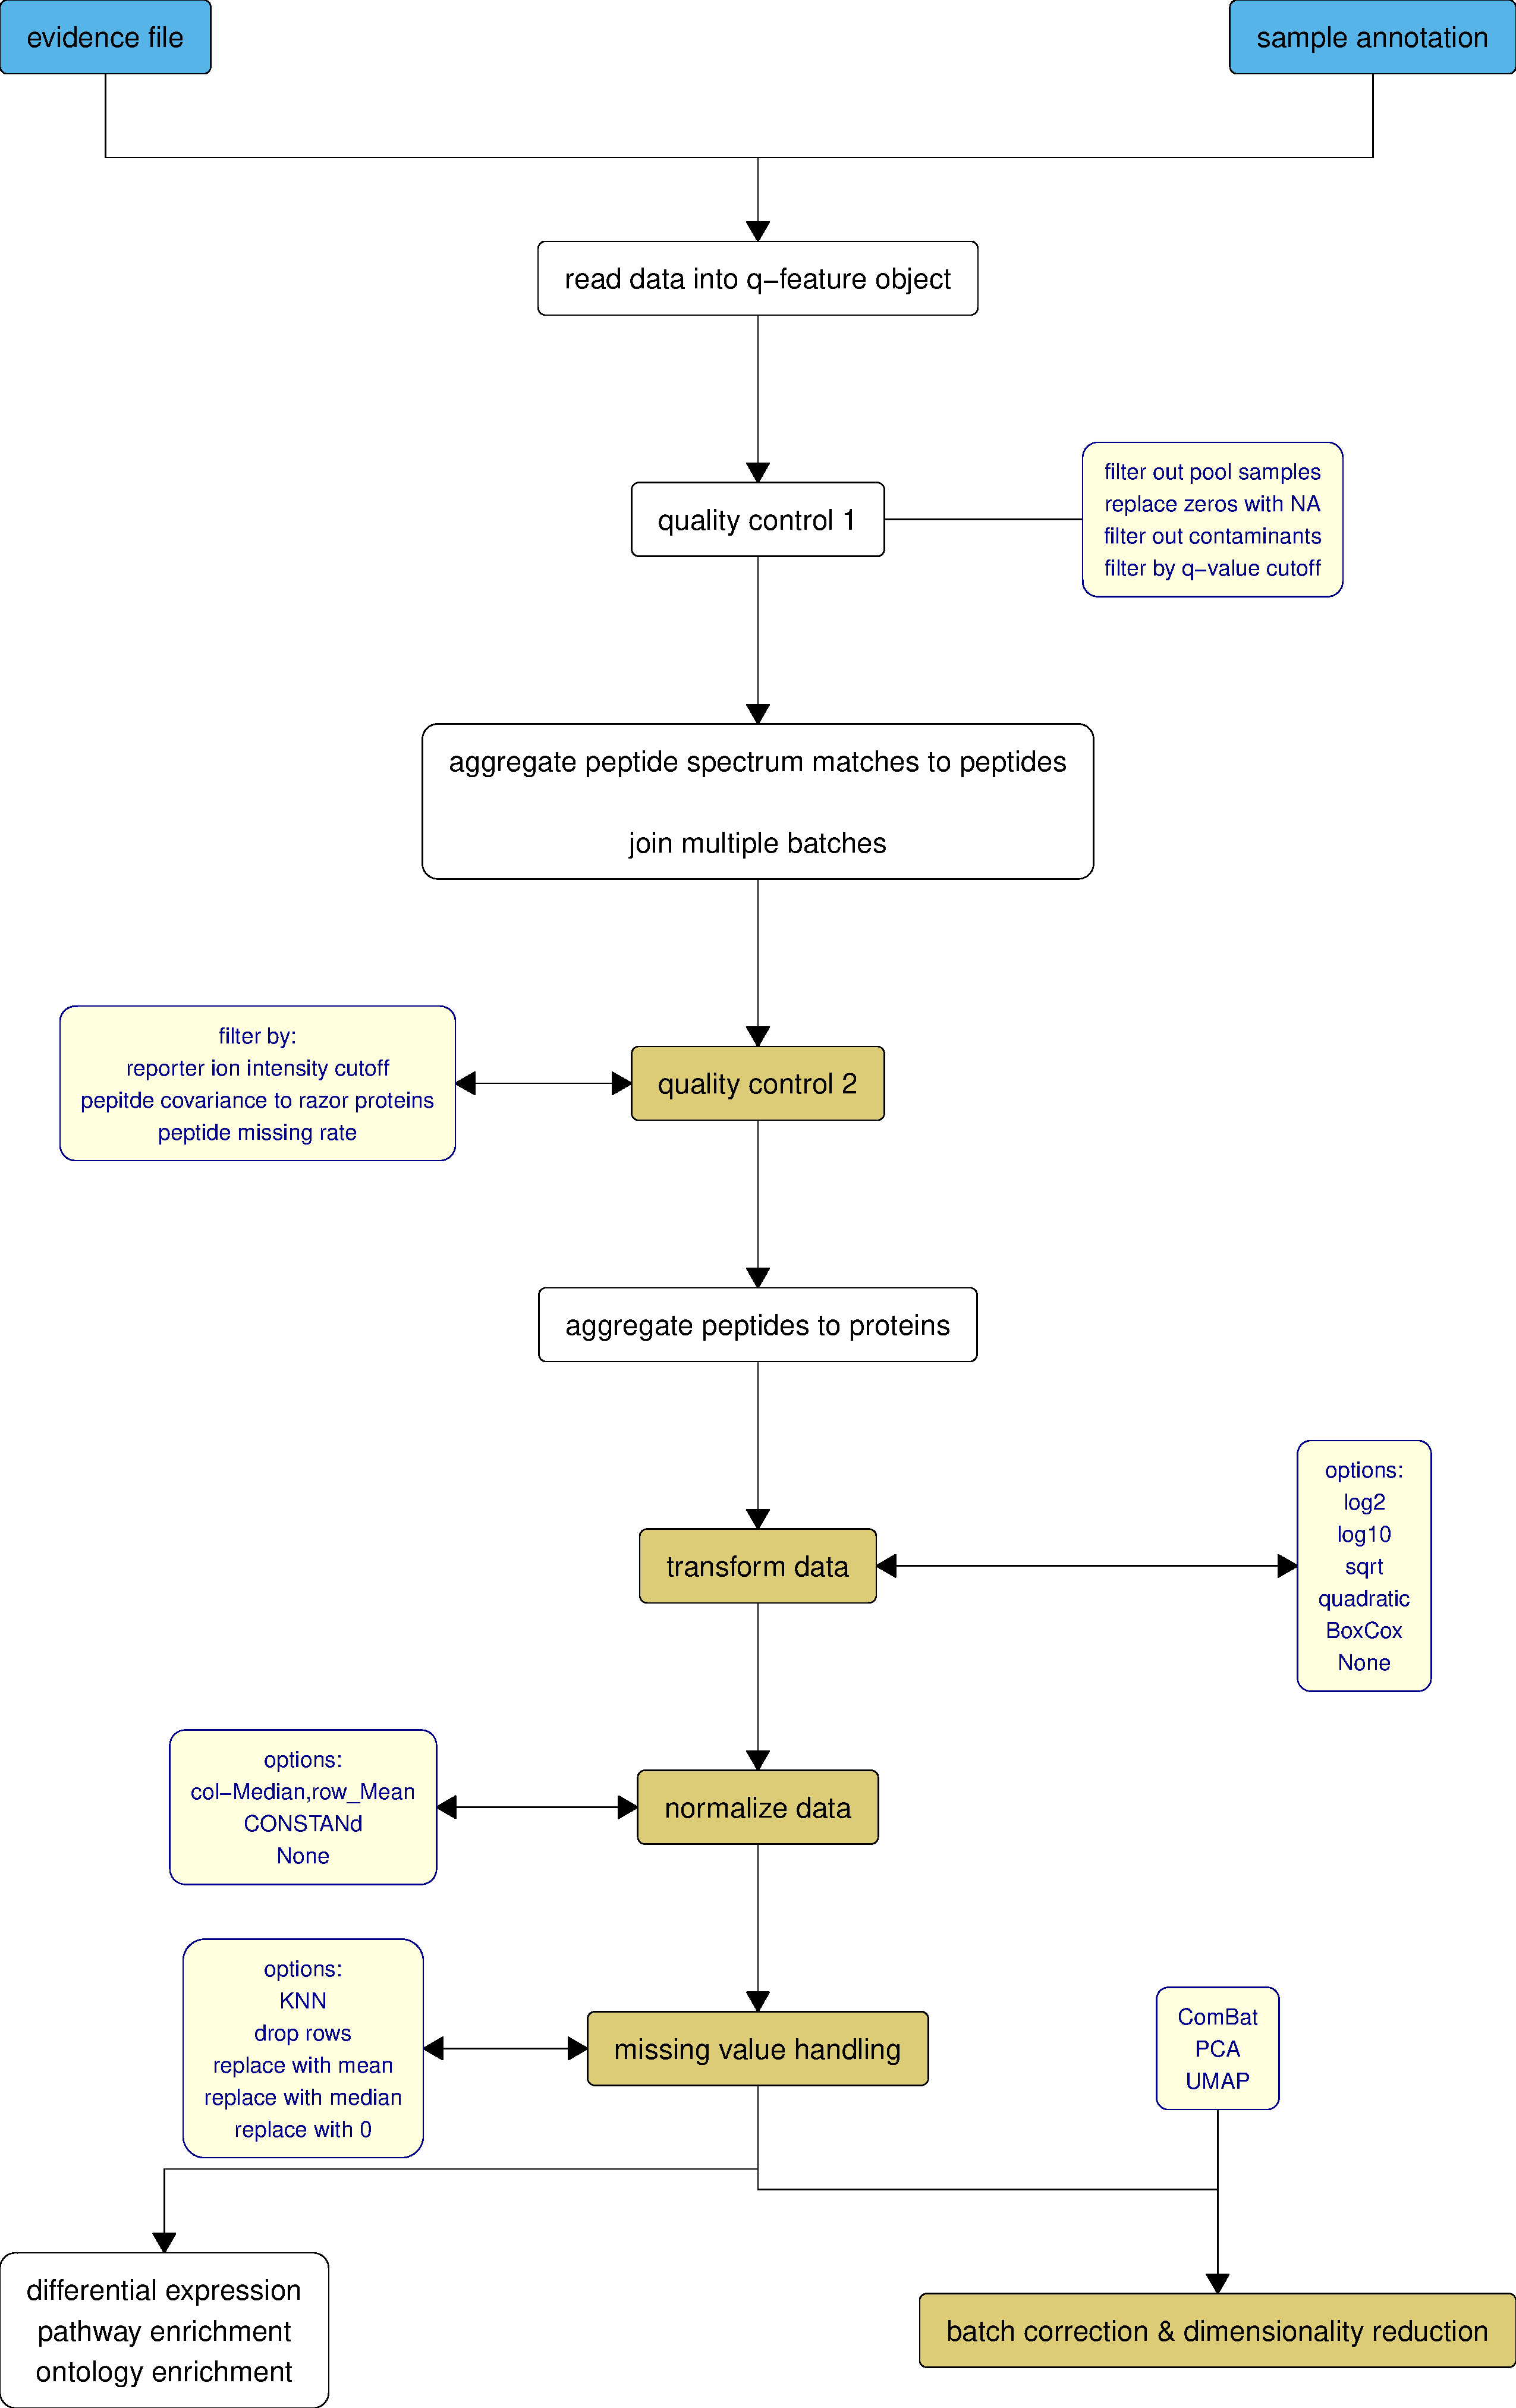
\includegraphics{Thesis_files/figure-latex/data_processing_pipeline_flowchart_vertical-1} 

}

\caption{Flowchart presenting the processing by ProteoScanR}\label{fig:data_processing_pipeline_flowchart_vertical}
 \endfigure\egroup

\hypertarget{processing-the-data}{%
\subsubsection{Processing the data}\label{processing-the-data}}

Further analysis is done with R and respective bioconductor packages.
Please find version info in the appendix.

After processing MaxQuant creates a directory containing all results as
.txt file. The evidence.txt file includes all peptide to spectrum
matches (PSM) with their respective proteins and statistical parameters.

Example fo basic parameters and derivations include:

\begin{itemize}
\tightlist
\item
  Peptide sequence
\item
  Mass to charge ratio (m/z) for all scans (eg. MS1, MS2)
\item
  Retention time
\item
  Precursor Ion Fragment
\item
  Fraction of total spectrum
\item
  Base peak fraction
\item
  Reporter intensity (RI)
\item
  Posterior error probability (PEP)
\end{itemize}

\hypertarget{object-oriented-programming}{%
\subsubsection{Object oriented
programming}\label{object-oriented-programming}}

In order to streamline the analysis of multiple experiments, object
oriented programming was applied. The approach in R is to create a so
called Q-feature object, which contains all variables and metadata in a
hierarchical structure. The structure enables sub setting for further
analysis \citep{Vanderaa2021}.

\hypertarget{zero-values}{%
\subsubsection{Zero values}\label{zero-values}}

Peptides with low abundance are often set to zero during analysis.
However, assigning a value of zero may incorrectly suggest that the
sample does not contain the respective peptide. Given that it is highly
unlikely for a biological cell of a comparable type and function to not
contain a particular protein, replacing the zero value with ``not
applicable'' (NA) is crucial for understanding and interpreting MS data.
NA values will be managed in missing value handling later on the protein
level.

\hypertarget{exclude-reverse-matchescontaminants}{%
\subsubsection{Exclude reverse
matches/contaminants}\label{exclude-reverse-matchescontaminants}}

Peptide sequences matching to the reverse protein sequences (=decoy
database) are considered as possible contaminants. These matches will be
excluded from further analysis.

\hypertarget{filter-according-to-precursor-ion-fraction-pif}{%
\subsubsection{Filter according to precursor ion fraction
(PIF)}\label{filter-according-to-precursor-ion-fraction-pif}}

During mass spectrometry, the ions detected in MS1 are further
fragmented through collision during multiple MS runs. The resulting
product ions are derived from precursor ions (also known as mother ions
or parental ions). Contaminant peptides can co-migrate in this process
and were distinguished by the lower fraction of their respective
precursor ions \citep{Tannous2020}. These peptides need to be filtered
out during the analysis pipeline. A cutoff value, referenced in the
SCoPE2 pipeline \citep{Specht2021}, is applied in the user interface,
but it can be adjusted.

\hypertarget{filter-by-q-value}{%
\subsubsection{Filter by q-value}\label{filter-by-q-value}}

The next step for quality control is the exclusion of samples with a
high false discovery rate (FDR). When applying multiple statistical
testing (e.g.~t-Test) the obtained p-values can be considered as biased,
because the probability to observe a significant will iteratively
increase with each test performed. Corrections in statistics are an
approach to compensate for the multiplicity of testing. There are many
ways to do this compensation like the Bonferroni method or
Benjamini-Hochberg`s FDR. In Mass spectrometry the common ``way to go''
is calculating a false discovery rate, by dividing false PSMs (=hit of
the decoy database) through the total number of PSMs above the
peptide-spectrum matching score. The peptides spectrum matching score is
defined as \(-10 * log(p)\). Whereas the p-value is defined that the hit
is done by chance. The calculation of the score is highly dependent on
the data acquisition method used. MaxQuant uses Andromeda, an integrated
search engine. Proteome Discoverer from Thermo Fisher utilizes different
engines such as Mascot or Minora. As published by J.Cox in 2011 Mascot
and Andromeda showed similar performance when comparing FDR values as a
function of coverage. However the observed performance can be lower when
dealing with a decreased coverage \citep{Cox2011}.The threshold for
accepting an FDR of an individual PSM is described as q-value.

\hypertarget{peptide-spectrum-match-psm-aggregation-to-peptides}{%
\subsubsection{Peptide spectrum match (PSM) aggregation to
peptides}\label{peptide-spectrum-match-psm-aggregation-to-peptides}}

In data science, aggregation refers to a row-wise operation that merges
data based on a particular column using a specific function. In the
context of processing from PSMs to unique peptides, the desired column
is the PSM sequence. To account for different distributions across
multiple assays, the median of the channel is used as the function to
aggregate multiple matches into one.

\hypertarget{join-assays}{%
\subsubsection{Join assays}\label{join-assays}}

Sample size is often a limiting factor in hypothesis testing. A strict
quality control and the fact that TMT reagents are only available up to
18-plex can reduce the number of observed samples below the critical
threshold, leading to an early end of analyses. To overcome this
limitation, the provided software is capable of processing multiple runs
simultaneously, allowing for testing of multiple batches and increasing
the number of samples that can be included in the analysis. For further
processing the runs are joined in one object at the peptide level.

\hypertarget{calculate-median-reporter-ion-intensity-ri-and-filter}{%
\subsubsection{Calculate median reporter ion intensity (RI) and
filter}\label{calculate-median-reporter-ion-intensity-ri-and-filter}}

Columns which do not meet the desired intensity can be filtered by a
threshold set on the RI. The median RI can also be used to check if an
entire channel has a lower detection level. This can be due two reasons.
One is the expression level of the given proteins in a cell. Meaning,
that the expression of the observed cell type is simply lower than the
other type. Another one could be a spillage of TMT detection in other
channels due incorrect or missing correction of the TMT isotopes. The
correction values can be found on the vendor`s webpage (in this case
Thermo Fisher) and correction needs to be set up in MaxQuant.

\hypertarget{calculate-median-coefficient-of-variation-cv-and-filter}{%
\subsubsection{Calculate median coefficient of variation (CV) and
filter}\label{calculate-median-coefficient-of-variation-cv-and-filter}}

Depending having a bulk sample or single-cell sample choosing a minimum
of observed peptides and a cutoff value for the CV, changes the level of
confidence in the peptide data. The coefficient of variation of a
peptide is considered as the ratio of the standard deviation to the mean
and describes the relationship of the observed peptide signal over
multiple proteins (=razor proteins). Peptides having a high coefficient
of variation over many razor proteins are considered as noise and need
to be filtered out before statistical analysis.

\hypertarget{remove-peptides-with-high-missing-rate}{%
\subsubsection{Remove peptides with high missing
rate}\label{remove-peptides-with-high-missing-rate}}

Although missing value imputation can be performed during the analysis
of multiple batches, peptides with missing detections across channels
can be problematic for quantification. The proteomic composition of a
biological sample is similar between replicates and even across groups.
However, the threshold of missingness (described as a fraction of the
row) can be set in the user interface and adjusted.

\hypertarget{aggregation-of-peptides-to-proteins}{%
\subsubsection{Aggregation of peptides to
proteins}\label{aggregation-of-peptides-to-proteins}}

Similar to the already explained previous aggregation step the peptides
will be further processed into their respective proteins after the
quality control on the peptide level is performed. Finally an expression
matrix for every protein and their respective channel column is
returned. Each channel refers to a sample and contains the intensities
of each protein found in the biological specimen.

\hypertarget{transformation-of-protein-expression-data}{%
\subsubsection{Transformation of protein expression
data}\label{transformation-of-protein-expression-data}}

Data transformation applies a function to each value of a matrix or
array, so that: \[
y_i = f(x_i)
\] Depending on the distribution of the values in the observed
expression set, different transformations can be applied to fulfill
assumptions for statistical testing. In the shiny application, various
procedures are implemented and can be further expanded upon request from
the user. The macrophage analysis done by Specht et al.~mentioned in
their SCoPE2 publication \citep{Specht2021} uses the logarithm to the
base 2 to spread a compacted distribution and remove skewness in the
dataset. This transformation was used as a reference when comparing
methods. However, using the logarithm to the base 10 may be an easy way
to recalculate expression data in the mind and will also be facilitated
by other transformation methods such as the boxcox method, which is also
implemented in the application. When observing a wide distribution of
small and large values of the expression set in a histogram, a square
root transformation can help increase the variability of smaller values
and decrease the variability of larger values. Depending on the
distribution, the user has to decide which transformation to consider
and verify that statistical assumptions are met after application with
visualizations such as histograms, qq-plots, and MA-plots. For
statistically inexperienced users, the boxcox transformation can help
with this decision. Developed in 1964 by Box and Cox \citep{Sakia1992},
this method applies a linear model against 1 on the data to determine
the statistical parameter lambda by the maximum likelihood method. The
log-likelihood method takes the 95\% confidence interval for the
parameter lambda and the final lambda is chosen as the value with the
highest log-likelihood value.

\begin{center}
\begin{tabular}{l r}
$\lambda$ & Transformation \\
-2 & $\frac{1}{x^2}$ \\
-1 & $\frac{1}{x}$ \\
-0.5 & $\frac{1}{\sqrt{x}}$ \\
0 & $\log{x}$ \\
0.5 & $\sqrt{x}$ \\
1 & $x$ \\
2 & $x^2$
\end{tabular}
\end{center}

Depending on the size of lambda, a certain function will be
automatically applied to each value of the expression set in order to
introduce normality. In terms of usability, the boxcox method is the
most efficient transformation method, taking the decision of which
calculation to apply away from the user.

\hypertarget{normalization}{%
\subsubsection{Normalization}\label{normalization}}

The term normalization is ambiguous in data-science and will be
explained briefly in this chapter. Starting with converting the data to
the Z-distribution (Gaussian result), where 0 represents the mean and 1
represents the standard deviation, in vectorization every feature (or
protein) is represented as a vector that points in a specific direction
in the unit sphere, normalization can have different meanings.
Normalization is considered as part of the scaling procedure and ensures
that every feature contributes equally to the statistical model and
hinders large values from biasing the model in a particular direction.
However, this could also have negative consequences for the modeling
procedure, as it may reduce the impact of important features on the
dataset. Depending on the algorithms later used in the data processing,
the method of choice for normalization can change the results
significantly. The K-nearest neighbor (K-NN) clustering algorithm, for
instance relies on the distances between distinct data points by
minimizing variance of the squared euclidean distances. This method will
be applied in the missing value imputation, which will be the next step
applied to the data. The first normalization method available in the
user interface is column-wise median and row-wise mean normalization.
This method was chosen by Specht et al in the SCoPE2 publication 2021
\citep{Specht2021} and worked as a reference during the development
process to benchmark other methods. When dividing each value of an
expression set by the median of the particular column, the procedure is
considered as a column-wise median normalization. Although the
mean-normalization works the same way but takes the mean as the second
variable. In the analysis pipeline both procedures were applied on the
dataset. However when the logarithm as the transformation method was
chosen as transformation method, ProteoScanR automatically switches from
a division to a subtraction, since:
\(\log_a \left(\frac{u}{v}\right)=\log_a u-\log_a v\). After applying
this normalization method, each value can be interpreted as a distance
or fraction of the mean or median of the corresponding column or row,
enabling fair comparisons between features and samples. The second
method for normalization included is the CONSTANd method, which was
proven suitable for relative quantification in the field of proteomics
\citep{Maes2016, VanHoutven2021}, but can also be applied on RNAseq
data. CONSTANd uses a technique called matrix raking, which employs the
RAS algorithm. The expression set reflects the non-negative real
\((m, n)\) matrix \(A\) were the bi proportional constrained matrix
problem will be solved by finding the \((m, n)\) matrix \(B\) which
equals to \(diag(x) * A *diag(y)\) . Whereas \(x \in \mathbb{R}^{m}\)
and \(y \in \mathbb{R}^{n}\). The solution to this problem involves
finding the row sum of \(B=u_i\) and the column sum of \(B=v_j\), where
\(i\) and \(j\) denote the row and column indices of the matrix,
respectively \citep{Bacharach1965}. In other words, the matrix will be
alternatively manipulated on rows and columns until the mean of both
equals 1. In order to apply the method and yield true results, one has
to consider 3 major assumptions between sample types. This assumption
can be observed in the MA-plot which indicates the differences of two
samples. Given the intensities of two samples, \(R\) and \(G\),
visualized on a graph with the x-axis as \(M=\log_2(\frac{R}{G})\) and
the y-axis as \(A=\frac{1}{2}\log_2(RG)\). A comparison between all
sample types of identically processed sets is needed before calculation
and the assumptions must be fulfilled.

\begin{itemize}
\item{\textbf{1}} \textbf{The majority of proteins are not differentially expressed}
\\Density of the dots decreases when looking from the middle of the cloud towards the edges.

\item{\textbf{2}} \textbf{Up- and downregulation is balanced around the mean expression}
\\The scatterplot of the data points is symmetrical around the mean on the horizontal axis. 

\item{\textbf{3}} \textbf{Systematic bias correlates with the magnitude of expression}
\\The symmetry axis is approximately horizontal.

\end{itemize}

If the MA-plot does not visualize any of these violations the CONSTANd
method can be applied on the dataset and the biological meaning of the
sample types can be assessed. The method is utilized by the bioconductor
package handler. Another method developed in the application is the
quantile normalization. Quantile normalization is performed over all
columns, equalizing statistical parameters such as inter quartile range,
median and mean. However the application of this method is only suitable
if the number of differentially expressed proteins is approximately
equal over sample types. Otherwise statistical power could be lost by
removing fine deviations \citep{Zhao2020}. For the quantile
normalization method the package limma was utilized. Quantile
normalization ranks protein expression by magnitude, then averages the
expression values occupying the same rank and substitute the inital
value with the average. However if the dataset already consists of
balanced features and samples or the user wants to benchmark the methods
applied, normalization can be skipped also, by setting to ``none''.

\hypertarget{missing-value-handling}{%
\subsubsection{Missing value handling}\label{missing-value-handling}}

When analyzing multiple batches simultaneously, it is possible to
encounter situations where a particular protein is not detected in one
of the batches. From a biological perspective, it is highly unlikely
that a cell completely lacks a single protein, as it would imply a
complete loss of function for that protein. Therefore, an intensity
value of 0 is close to impossible for most proteins. In order to handle
this dark space in the expression set, several methods can be chosen in
the application. A variety of function employs replacing the missing
values with the mean or median of the rest of the matrix. This procedure
introduces no bias in the data if the missingness is low, although
differential expression for the sample carrying the missing feature can
not be expected as well. Even a more conservative approach is dropping
the rows for the feature with the missing value in one of the observed
samples. A common practice in proteomics is utilizing the K-nearest
neighbor algorithm (=KNN), which imputes the missing values by a
euclidean metrics of the neighboring values in the columns where the
feature is not missing. \(K\) denotes for the count of neighboring
values of a gene and can be selected upon preference. The euclidean
distance between two points is defined as \(d = \sqrt{a^2 * b^2}\), the
\(K\) nearest neighbors average value will be assigned to the intensity
of the missing feature. Since the average is a statistical metric which
can be biased easily by skewed distributions, normalization is an
important task before performing missing value imputation. KNN was
benchmarked for the regression of protein abundance intensities and
showed an Area under the Curve (AUC) above 0.7 when testing on a human
proteome test set \citep{Lan2013}.

\hypertarget{batch-correction}{%
\subsubsection{Batch correction}\label{batch-correction}}

Since mass spectrometry experiments are highly influenced by several
factors, such as sample processing, the technician, manufacturer and
production of the device, the reagents etc., working in multiple batches
introduces further variance in the protein data. This variance would
overshadow the biological differences across sample types when
performing dimensionality reduction. A common misconception in biology
is, that batches need to be corrected before differential expression
analysis, which is the final aim of ProteoScanR. It appears convenient
to remove the batch effect before performing any statistical analysis,
which is in turn prone to errors especially if the sample groups are not
split equally between batches. In this case, group differences influence
the batch effect reducing statistical power after the correction. These
both effects are so called interdependent. The opposite could happen if
the experimental design is heavily unbalanced leading to group
differences induced by batch correction. Finally it is recommended to
include the batch factor should in the linear model as a co-factor and
statistically quantify it \citep{Nygaard2016}. However it could be of
interest to observe biological relevance of the factor of interest in
the dimensionality reduction visualization, so a batch correction option
was included to meet this need. To address the non-biological
experimental variations, also known as technical factors, the R package
sva \citep{Leek2012} with the ComBat function \citep{Johnson2007} was
used. The expression of a gene \(g\) for the batch \(m_i\) and sample
\(j\) can be defined as
\(Y_{ijg} = a_{g} + X\beta_{g} + \gamma_{ig} + \delta_{ig}\epsilon_{ijg}\),
where \(\gamma\) and \(\delta\epsilon\) represent the systematic error
caused by the batch. The Bayesian framework is employed to remove this
systematic error by shrinking the effect and pooling information over
the features \(g\). Ideally the effects \(a\) and \(\beta\) remain as
natural as they are and should reflect the true biological difference
between experimental obtained samples or groups. Before applying batch
correction, the data is standardized using Z-transformation. By the
method of moments (= the mean and the variance) the two batch effect
parameters \(\gamma\) and \(\delta\epsilon\) were estimated and can be
subtracted from each value for the particular feature driving
statistical moments at a comparable level between batches. The ComBat
function allows the user to specify a desired effect, which represents
the actual biological variance to be preserved while removing
non-biological variance. This is achieved by constructing a design
matrix, which is provided as prior information about the dataset within
the Bayesian framework. However, in cases of poor experimental design,
the factors contributing to unwanted and desired variation may be
confounded. In the worst case, if only one sample type per run is
observed, it becomes challenging for the program to distinguish between
batch-induced variance and biological variance. In such cases, the user
is advised to adjust the experimental layout for future experiments. The
detection algorithm for confounding effects is facilitated by QR matrix
decomposition. The matrix \(A=QR\) is decomposed into an orthogonal
matrix \(Q\) and an upper triangular matrix \(R\). By comparing the rank
of matrix \(A\) with the number of biologically relevant factors, it is
possible to determine the presence of confounding effects in the
dataset. The rank is defined as the maximum number of linearly
independent columns. The same approach is used in the limma package
\citep{Phipson2016} to identify non-solvable coefficients in
experimental designs.

\hypertarget{dimensionality-reduction}{%
\subsubsection{Dimensionality
reduction}\label{dimensionality-reduction}}

After cleaning the data and crystallizing from impurities such as noise
and unwanted effects, the biological differences between sample types
can be obtained. Proteomic data consists of multi dimensions (=features)
which are overall hard to understand by a glance. An approach to observe
the differences without a closer sight of exact effect on the
proteinaceous ensemble, but still keep a high level of information can
be dimensionality reduction. After the cleaning procedures any
additional effect caused by technical or biological replication should
be removed, however it could be found be highlighting according to the
particular factor. This makes the dimensionality reduction a useful tool
before starting any statistical analysis by checking for involuntarily
introduced bias.

\hypertarget{principle-component-analysis-pca}{%
\paragraph{Principle component analysis
(PCA)}\label{principle-component-analysis-pca}}

The most common approach in data science for any kind of high
dimensional data is the PCA. For ProteoScanR the bioconductor package
scater \citep{McCarthy2017} was used. Every principle component can be
understood as a vector pointing in a specific direction derived as the
eigenvector from the covariance matrix of the expression set. The
covariance matrix indicates for the co linearity between the variance of
all elements compared. After calculating the covariance matrix the
eigenvectors for the covariance matrix will be obtained by solving the
quadratic equations to obtain the eigenvalues \(\lambda\). Since
\(A v = \lambda v\) the eigenvector \(v\) can be obtained by solving the
equation for each element of the vector. The eigenvectors \(v\) never
changes is direction and explains the covariance within the dataset and
so also the mathematical differences between the samples. The
eigenvectors are sorted according to their eigenvalues in decreasing
order and therefore decreasing explained variance. For graphical
visualizations the principle components are plotted against each other.
The first two components, which explain the majority of variance in the
dateset highlight the difference between samples.

\hypertarget{uniform-manifold-approximation-projection-umap}{%
\paragraph{Uniform manifold approximation \& projection
(UMAP)}\label{uniform-manifold-approximation-projection-umap}}

UMAP \citep{McInnes2018} is a dimensionality reduction technique that
was developed in recent years and is based on Riemann geometry. It
shares similarities to the t-distributed stochastic neighbor embedding
(t-SNE) in terms of graphical visualization. Riemann geometry is a
mathematical framework that deals with three dimensional functions using
volumes, areas and vectors, which are also concept of topological data
analysis. Before performing UMAP, three assumptions need to be
considered:

\begin{enumerate}
\item There exists a manifold on which the data would be uniformly distributed.
$\rightarrow$ This assumption implies that the probability for each value in the biological dataset is the same.

\item The underlying manifold of interest is locally connected.
$\rightarrow$ In other words, similar samples will have a similar proteinaceous ensemble.

\item Preserving the topological structure of this manifold is the primary
goal.
$\rightarrow$ This means that the homeomorphic structure (the property of being able to transform one shape into another without tearing or gluing) is locally preserved, and local values in the dataset can be compared with each other.
\end{enumerate}

\citep{McInnes2018}

The UMAP algorithm begins by constructing a graph with a defined
neighborhood parameter, typically denoted as \(k\), which can be
selected computationally. UMAP employs the k-nearest neighbor descent
algorithm (NN-descent). Similar to the k-nearest neighbor algorithm
(KNN), used in the missing value imputation part of this project,
NN-descent recursively iterates to find the smallest distance to the
respective neighbors within the defined neighborhood size \(k\).
Increasing the value of \(k\) gradually strengthens the clustering of
the data, but at a certain point, fine structure may be lost, and only
rough estimates of the underlying principle can be observed. The
mathematical graph in UMAP is defined by nodes connected by edges, with
each node internally connected to at least one other node. Edges are
distinguished from each other not only by their connection but also by
their importance, which is often referred to as weight. Whereas the
weight function is calculated as

\[w((x_i, x_{i_{j}})) = \exp(\frac{-max(0,d(x_{i},x_{i_{j}}-\rho_{i})}{\sigma_{i}})\]

and determine the parameter \(\rho\) for the weight function that:

\[\rho_i=\min \left\{ d(x_i,x_{i_{j}}) \,|\, 1 \leq j \leq k, d(x_i, x_{i_{j}}) > 0 \right\}\]

Furthermore \(\sigma\) will be set to meet the following conditions:
\[\sum_{j=1}^{k} \exp ( \frac{ -\max(0, d(x_{i}, x_{i_{j}}) - \rho_i)} { \sigma_i } ) = \log_2(k)\]
and acts as a normalization factor. The obtained graph \(\overline{G}\)
is called the fuzzy simplicial set which is obtained by approximating
the geodesic distance (= locally length-minimizing curve) of the data
points, leading to a topological approximation. The second phase of the
algorithm adjusts the layout of the weighted graph to a representative
view, but preserves the characteristics and shows the underlying
topological principle of the data. In order to obtain a visual
representation of the graph, the algorithm applies repulsive forces:
\[\frac{2b}{(\epsilon + ||y_i-y_j||_{2}^{2})(1+a||y_i-y_j||_{2}^{2b})}(1-w((x_i,x_j)))(y_i-y_j)\]
among vertices and attractive forces
\[\frac{ -2ab || y_i -y_j||_{2}^{2(b-1)} }{1+||y_i-y_j||_{2}^{2}} w((x_i,x_j))(y_i-y_j)\]
along edges. Where \(a\) and \(b\) are denoted as hyperparameters. By
iterating through possible conformations until converging towards a
local minimum with decreasing repulsive and attractive forces, the UMAP
reaches it`s aim to reveal the underlying properties of the data. The
application utilizes the bioconductor package scater for performing UMAP
\citep{McCarthy2017}.

\hypertarget{validation-of-the-methods-applied-to-the-dataset}{%
\subsubsection{Validation of the methods applied to the
dataset}\label{validation-of-the-methods-applied-to-the-dataset}}

For the validation of methods applied to the dataset, the mutual
information calculation is used to assess the impact of computations and
the information it carries. Mutual information, denoted as \(I(X;Y)\),
is a measure of the dependence or information shared between two
variables, \(X\) and \(Y\), in this case sample types. It is calculated
using the equation \(I(X;Y) = H(X,Y) - H(X|Y) - H(Y|X)\), where \(H\)
represents the entropy, \(H(X|Y)\) and \(H(Y|X)\) denote for the both
conditional probabilities and \(H(X,Y)\) for the joint entropy. Entropy,
as a concept in information theory, quantifies the level of disorder or
uncertainty associated with a random event. Events that are highly
likely to occur are considered less informative than events that are
more unexpected or less likely. In a Venn diagram \(I(X;Y)\) (the mutual
information) corresponds to the intersection of the two conditional
entropys \(H(X|Y)\) and \(H(Y|X)\). To calculate the mutual information
between two variables \(X\) and \(Y\) the above equation can be
alternatively expressed as
\(I(X;Y) = D_{KL} (P_{(X,Y)} || P_{X} \otimes P_{Y})\). \(D_{KL}\)
denotes for the Kullback-Leibler \citep{Kullback1951} divergence which
is a concept of relative entropy between two variables and tells us how
much 2 probability distributions differ from each other.
\(P_{X} \otimes P_{Y}\) represents the product of the marginals. The
underlying principle of divergence is the integral asymmetry in Bayesian
inference, which means that divergence does not satisfy the triangle
inequality. Differences are not the same depending on the starting
point. By comparing the mutual information before performing any
calculations with the mutual information calculated after the
computations, it is possible to assess whether the applied methods have
significantly altered the dependence or information content. The goal is
to choose a method which preserves the information contributed by each
biological sample type to the experiment. The R package ``infotheo'' is
utilized to perform the estimates for the entropy of the two variables.
Mutual information is returned as natural unit of information (=nat), a
measurement proportional to the to the Shannon entropy
(\(1nat = \frac{1}{ln2} shannons\)). Before calculating the pairwise
mutual information of the expression matrix, values were discretized
into bins with the discretize function of above package. The mutual
information is calculated within each sample type, and it can also be
calculated between a selection of sample types to determine if the
computations performed affect the information content. After that all
pairwise mutual information within the expression set before and after
ProteoScanR is obtained. The pairwise differences can be observed as a
boxplot for a particular sample type indicating the change in dependence
within and also compared to another sample type.

\hypertarget{statistics}{%
\subsubsection{Statistics}\label{statistics}}

\hypertarget{differential-expression}{%
\paragraph{Differential expression}\label{differential-expression}}

After visualizing the biological tendency in the dataset, the next step
is hypothesis testing. Several experimental designs can be tested
against the null hypothesis \(h_0\), which states that there is no
significant difference between the sample types. Before proceeding with
any statistical testing, it is important to observe the data using
either a quantile-quantile plot (qq-plot) or a histogram. The qq-plot
serves a vital role in exploratory statistics by visualizing whether two
datasets follow the same underlying distributions. In the case of
statistical preparation for parametric tests, the first distribution is
the dataset of interest, while the second dataset is the normal
distribution. If the dataset follows an exact normal distribution, the
values will align with the red line in the chart. However, values at the
ends of the distribution may deviate from the normality line, indicating
differentially expressed genes. These genes can be observed both in the
histogram and the qq-plot. Parametric statistical tests rely on the
assumption of normality in the data, which needs to be achieved before
building a model. To achieve normality, it is recommended to try various
combinations of transformation and normalization methods. By observing
the results in the plots, one can determine which combination of data
processing methods satisfies the conditions required for the tests.
However the limma method utilized in the statistics module shows great
robustness to imperfect normal distributed values \citep{Ritchie2015}.

To test for differential expression, the analysis utilizes the ``limma''
package from R Bioconductor \citep{Phipson2016}. This package employs a
linear model approach to determine the fold expression between sample
groups. Before initiating the analysis, two matrices need to be
computed. The design matrix identifies samples based on their sample
type and defines the experimental design. An algorithm within the
program's backend logic is utilized to automatically generate this
matrix according to the user's selection in the interface. The
expression matrix contains intensities for each identified protein and
is obtained at the end of ProteoScanR. By calling a function with the
design and expression matrices as arguments, the contrast matrix is
calculated, enabling the user to decide which comparisons to consider
and also perform tests on multiple factors. When observing multiple
batches at once, as already explained in the chapter batch correction
this effect needs to be taken into consideration when performing
differential expression analysis. This is done by the multi-factor
option in the user interface by selecting the batch as a co-factor and
inclusion in the design matrix. The advantage of this procedure is, that
the biological relevance of working in multiple batches can be
quantified and the publishing of false positive results avoided. The
multi factor option uses an additive model as a design matrix, whereas
continuous variables (such as size, weight etc.) can also be used to
build the statistical model.

The subsequent step involves creating a linear model between groups
using log-ratios of their expression values. In a two-way design, the
expression of the gene \(y\) can be explained as
\(Exp_{Y} = \beta_{0} + \beta_{1}X_{1} + \epsilon\), where \(\beta_0\)
represents the intercept, which can be interpreted as the mean
expression of the gene. \(\beta_1\) represents difference in mean of the
treatment (or condition) on the discrete or continuous variable
\(X_{1}\), and \(\epsilon\) acts as an error term. The interface allows
for additive models with multiple factors, allowing the user to add
factors according to various scenarios. For example, in a two-factor
model, it would look like:
\(Exp_{Y} = \beta_{0} + \beta_{1}X_{1} + \beta_{2}X_{2} + \epsilon\).
The principle remains the same for models with multiple factors. When
visualizing the linear model, the x-axis would represent the gene for
the sample types or other factors, whereas the y-axis would account for
the expression value. By drawing a line through the cloud of data points
the model is constructed by minimizing the quadratic distance to every
data-point, called the least-square method or also ordinary least-square
method. With the regression line the above mentioned equation can be
constructed.

Next the statistical module of the program performs an empirical Bayes
model utilizing the eBayes \citep{Smyth2004} function of the Limma
package. The eBayes function utilizes a moderated t-statistics following
t-distributed values. The advantage of this method over the posterior
odds is the reduction of hyperparameters to estimate used for the
modelling process, also called shrinkage. In this context, the
hyperparameters to estimate are the coefficient \(\beta_{gj}\) for gene
\(g\) and sample \(i\), as well as the variance \(\sigma^2_g\) across
genes \(g\). In the Bayesian approach, probabilities are updated after
obtaining new data, referred to as conditional probabilities. For
estimation, it is assumed that
\(\frac{1}{\sigma^2_g} \sim \frac{1}{d_{0}s^2_{0}} \chi^2_{d_{0}}\),
representing the prior information of the model. The probability for
\(\beta_{gj} \neq 0\) is denoted as \(p_j\), where \(p_j\) represents
the expected proportion of truly differentially expressed genes. The
expected distribution of log-fold changes follows the distribution
\(\beta_{gj} | \sigma^2_g , \beta_{gj} \neq 0 \sim N(0, v_{0j}\sigma^2_g)\).
The posterior mean of \(\sigma^2_g\) given \(s^2_g\) is calculated as
\(s^{-2}_g = E(\sigma^2_g | s^2_g) = \frac{d{0}s^2_{0} + d_{g}s^2_{g}}{d_{0} + d_{g}}\).
This is where the shrinkage occurs, as the posteriors affect the prior
values based on their respective sizes and degrees of freedom. The
moderated t-statistic is defined as
\(\tilde{t}_{gj} = \frac{\hat{\beta}_{gj}}{\hat{s}_{g}\sqrt{v_{gj}}}\).
Once the values of \(\tilde{t}\) and \(s^{2}\) are calculated, the
posterior odds are computed, providing the odds that a particular gene
is differentially expressed. The odds for gene \(g\) being
differentially expressed are denoted as
\(O_{gj} = \frac{p(\beta_{gj} \neq 0 | \tilde{t}_{gj}, s^2{g})}{p(\beta_{gj} = 0 | \tilde{t}_{gj}, s^2{g})}\),
where the numerator represents the probability that the gene is
differentially expressed, and the denominator represents the probability
that the gene is not differentially expressed \citep{Smyth2004}.

Limma outputs a table with all proteins, their respective logfold
change, p-values and adjusted p-values. The user can choose different
methods for the correction of the p-values, which is necessary when
testing the same hypothesis multiple times. A common method in omics
studies is the false discovery rate (=fdr) by Benjamini Hochberg
\citep{Benjamini1995}. By ranking all the p-values from smallest to
largest the p-values are adjusted sequentially using the formula
\(p_(i) = \frac{r_i}{m} Q\). The rank in the p-value table is denoted as
\(r_i\) , \(m\) reflects the total number of tests and \(Q\) represents
false discovery rate which is set to 5\%. The second option to choose is
the Benjamini \& Yekutieli (=BY) \citep{Benjamini2001}method, which is a
further development of the fdr by the same statistician and has a wider
range of application based on the dependencies for the test. The third
and most conservative option is the Holm method \citep{Holm1979} which
controls the error sequentally in a family wise manner, which is
considered as traditional in regards to the above mentioned experimental
wise error rates. The above mentioned correction methods are ordered in
the way from the most liberal to the most conservative one. The
selection is supposed to give the user the possibility questioning
results on multiple levels.

\hypertarget{protein-set-enrichment-analysis}{%
\subsubsection{Protein set enrichment
analysis}\label{protein-set-enrichment-analysis}}

After differential expression the upcoming question could be, in which
context the up or down regulated proteins are. Enriched pathways can be
understood as an over-representation (ORA = over-representation
analysis) of proteins within a specific set. This set can be a pathway
or a selection of common denominators in biological contexts, such as
cell types or oncological factors. The statistical testing to identify
the overabundant proteins of a specific set is similar to a \(\chi^2\)
test developed by Karl Pearson \citep{Pearson1900} or the exact Fisher
test \citep{Sprent2011} for tables with 4 fields in small sample sizes.
Within the list are all truly differentially expressed genes, an
annotation is the identification of a protein in the desired biological
context. The table is expected to be populated by the values as follows:

\begin{center}
\begin{tabular}{|c|| c| c|| c|} 
 \hline
   & in list & not in list & totals \\ [0.5ex] 
 \hline\hline
 with annotation & (A+B)(A+C)/N  & (A+B)(B+D)/N & A+B \\ 
 \hline
 without annotation & (C+D)(A+C)/N & (C+D)(B+D)/N & C+D \\
 \hline
  & A+C & B+D & N \\
 \hline
\end{tabular}
\end{center}

Under the null hypothesis \(H_{0}\) states that the distribution and
population of the table is random and there is no clear tendency with
significant evidence. Against that the alternative hypothesis \(H_{A}\)
says that there is an underlying tendency the table is populated. This
leads to the test statistics, the observed values (=\(O\)) in the table
are significantly different to the expected
(=\(E=\frac{(A+B \lor C+D)}{N}\) ones. One approach is approximating
\(\chi^2= \sum_{i=1}^{n} \frac{(O_i - E_i)^2}{E_i}\) and deriving the
p-value by the area under the density curve of the \(\chi^2\)
distribution \(Q = \sum_{i=1}^{k} Z_{i}^{2}\). In the distribution \(k\)
is defined by the degrees of freedom (=df), what can be obtained by
\(k=(columns-1)*(rows-1)=df\) of the table. Another approach to obtain
an exact p-value would be Fisher`s exact test, which states that the
margins are distributed according to the hypergeometric distributions.
The test statistic leads directly to the p-value with no need for
approximation:
\(p=1-\sum_{i=0}^{A-1}\frac{\binom{B}{i}\binom{D-B}{A+C-i}}{\binom{D}{A+C}}\)
Here D denotes either for the background distribution which can be the
total number of proteins obtained in the experiment, all proteins with
annotation or a custom selected background. The background indicates all
proteins which could be positive tested for in the observed sample. The
above mentioned three options are implemented in the user interface.
After obtaining the p-values for each protein set, the subsequent
critical step involves the correction for multiple testing, considering
the inherent risk of false positive results. Multiple testing correction
methods adjust the significance thresholds to account for the increased
probability of detecting false positives when performing multiple
statistical tests. In this protein set enrichment analysis, the user is
provided with a selection of established correction methods, akin to
those commonly utilized in the field of differential expression
analysis, ensuring robust and reliable interpretation of the results.
Once the enriched protein pathways are determined, they can be visually
represented using bar or dotplots, and a network of the found pathways.
In the network ontologies are depicted as nodes, whereas edges show the
strength of the interaction by thickness corresponding to the number of
associated proteins.

\hypertarget{pathway-enrichment-analysis}{%
\paragraph{Pathway enrichment
analysis}\label{pathway-enrichment-analysis}}

The pathway enrichment analysis is performed using the R Bioconductor
package clusterProfiler \citep{Wu2021}. The analysis utilizes the entire
``Kyoto Encyclopedia of Genes and Genomes'' (KEGG) database, which is
accessed through a function that maps the UniProt IDs to corresponding
pathways.

\hypertarget{custom-ontology-based-protein-enrichment-analysis}{%
\paragraph{Custom ontology based protein enrichment
analysis}\label{custom-ontology-based-protein-enrichment-analysis}}

For custom ontologies the protein enrichment analysis is done using the
R bioconductor package piano \citep{Vaeremo2013}. In opposite to the
pathway enrichment, piano maps proteins to a pre-selected gene
collection set, which can be either downloaded from gsea-msigdb.org or
custom made for the particular experiment and explains conditions,
phenotype or other desired properties. For statistical testing the above
explained Fisher exact test is used.

\newpage

\hypertarget{results}{%
\section{Results}\label{results}}

To begin using the application, the first step is to upload the
tab-delimited evidence file and the sample annotation file. Once these
files are uploaded, the application is ready to run with default values.
The default settings are preconfigured for an initial analysis, and any
further adjustments or fine-tuning can be made in subsequent steps of
the analysis process.

\bgroup  \origfigure[H] 

{\centering 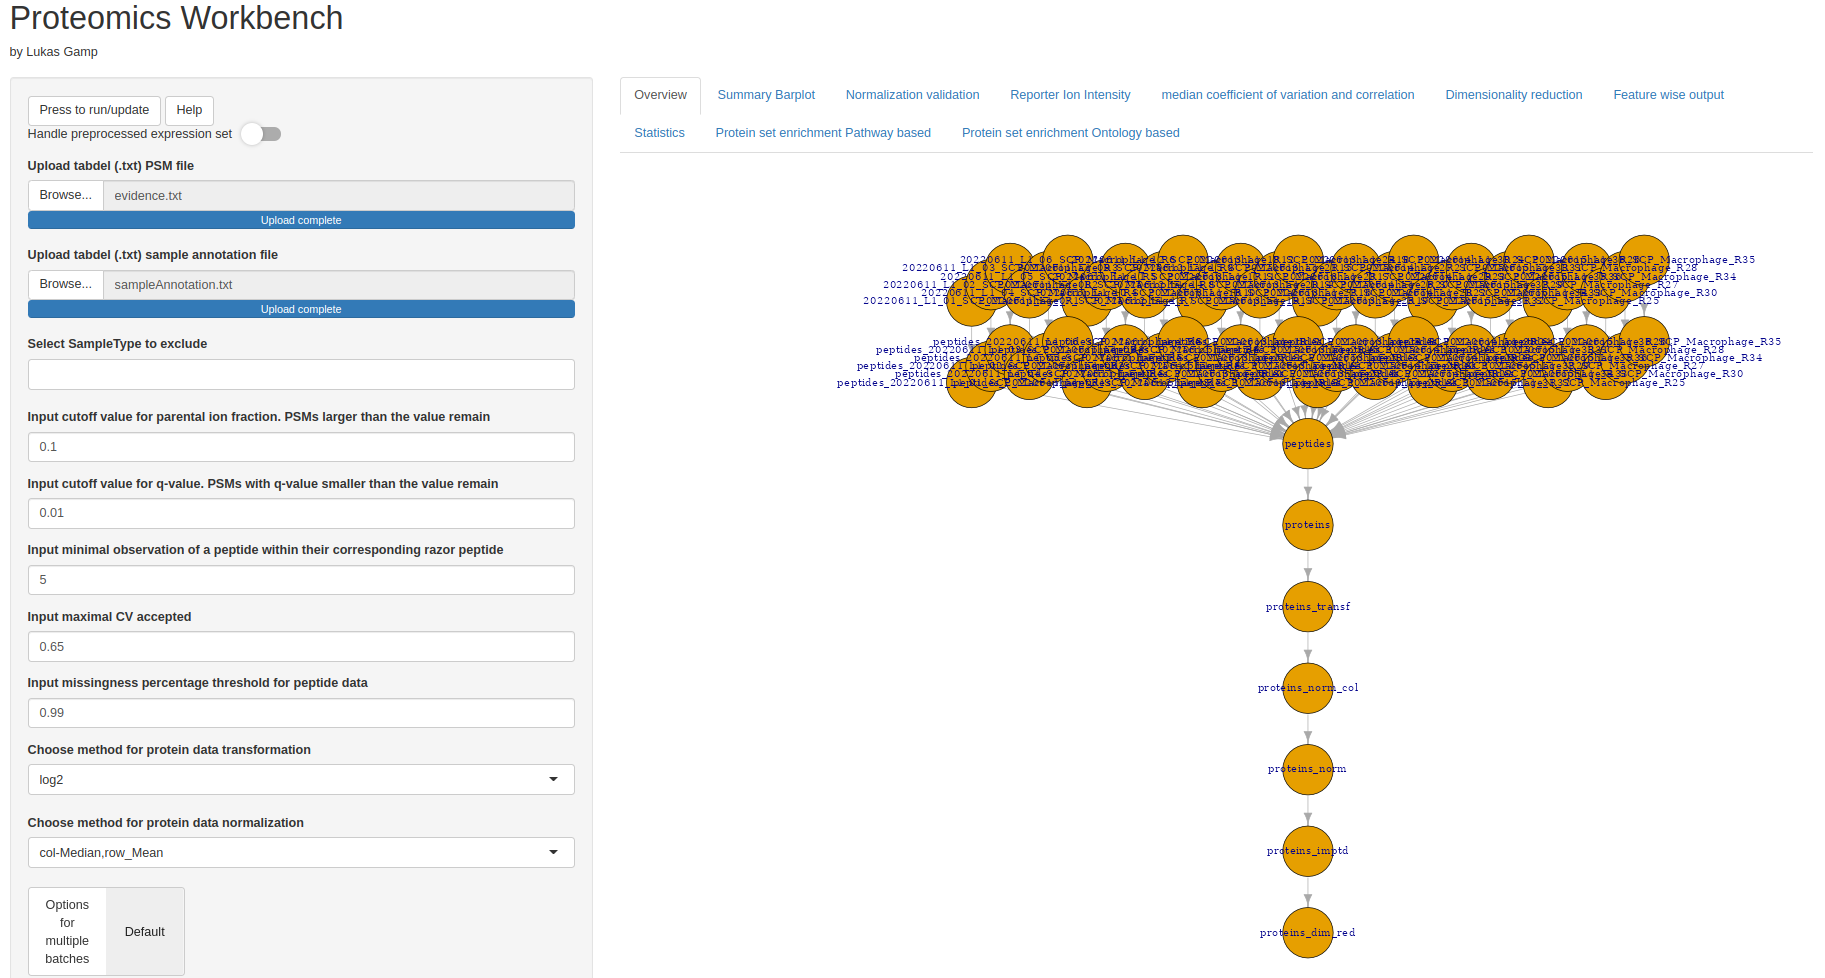
\includegraphics[width=1\linewidth]{screenshots/overview} 

}

\caption{Summary showing the process of the analysis pipeline}\label{fig:ui_summary}
 \endfigure\egroup

After a runtime of 2 minutes on the 4 core laptop the data is ready to
visualize. On the left side of the user interface, users can find the
analysis pipeline settings that can be adjusted. Once the desired
changes are made, they can be applied by clicking the update button.
This allows users to observe the direct impact of the applied changes on
the dataset. In the summary visualization, it may appear cluttered due
to the processing of 36 files. In smaller datasets, the nodes of the
network graph can be more easily distinguished and understood. When
running the application with SCoPE2 \citep{Specht2021} reference
cutoffs, the following results were visualized.

\newpage
\bgroup  \origfigure[H] 

{\centering 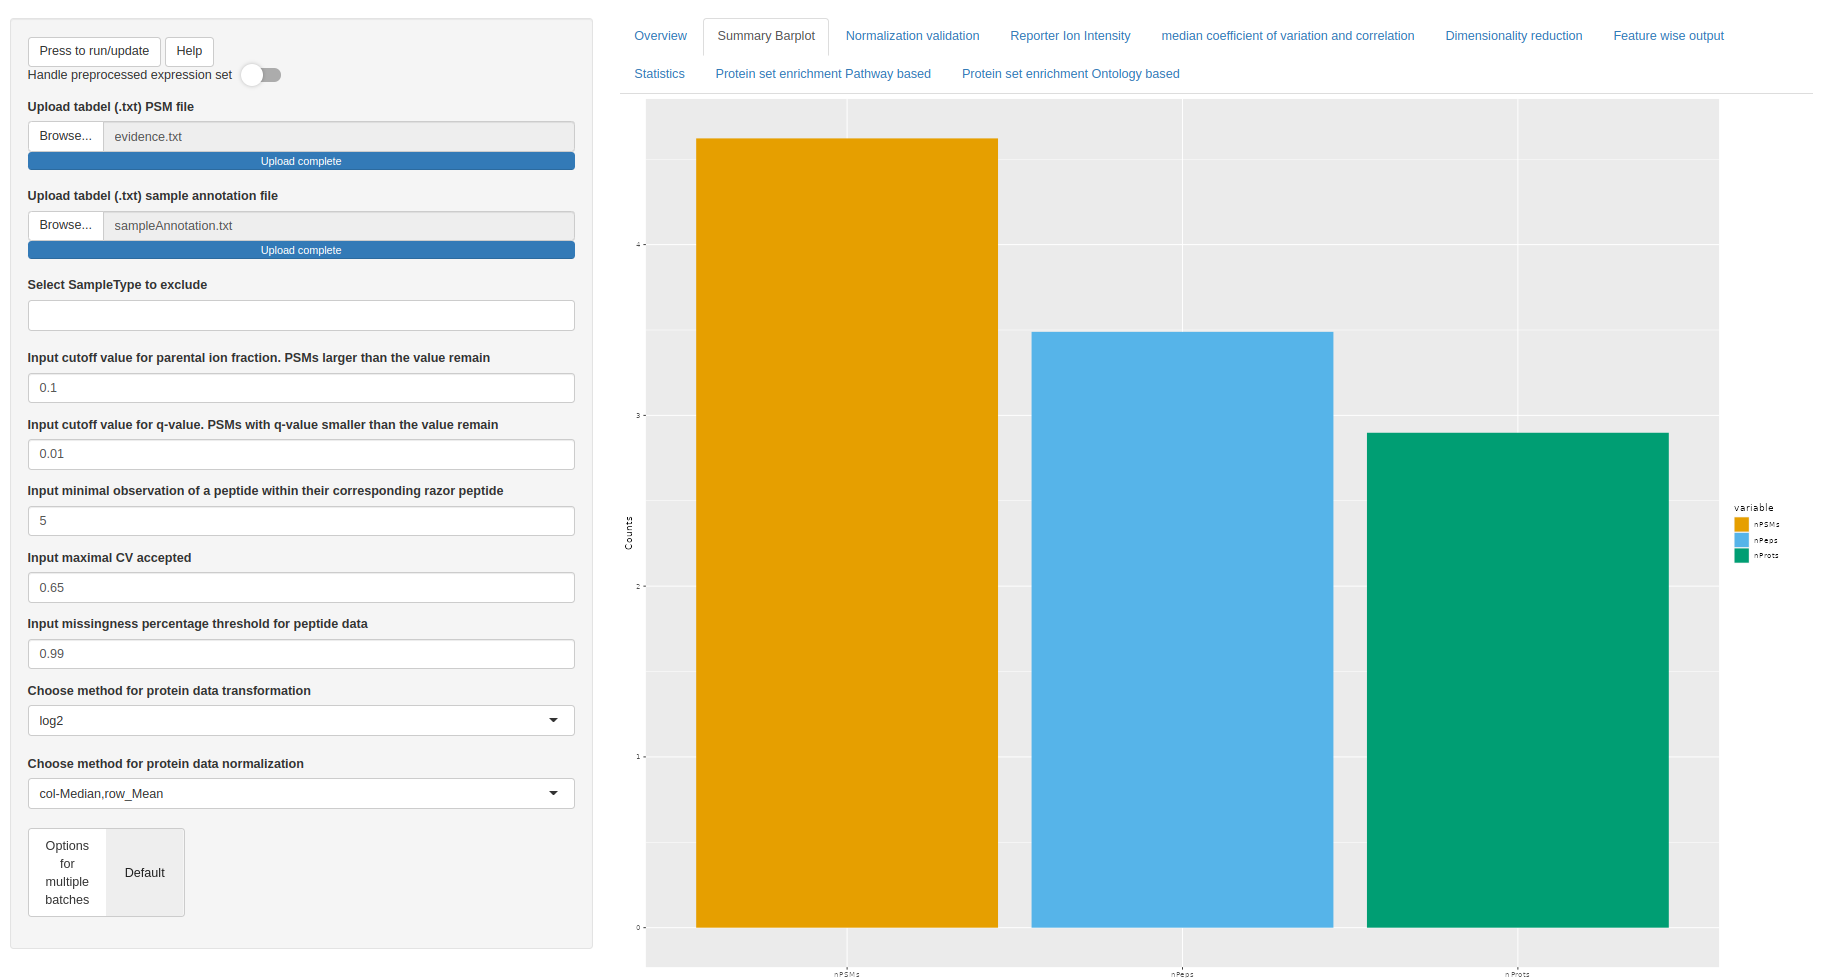
\includegraphics[width=1\linewidth]{screenshots/numbers_default} 

}

\caption{Barchart showing the number of peptide spectrum matches, peptides and proteins}\label{fig:ui_numbers_default}
 \endfigure\egroup

The default settings of the analysis pipeline resulted in a total number
of unique proteins below approximately \(10^3\), which were aggregated
from around \(10^{3.5}\) peptides. Before these peptides were aggregated
over approximately \(10^{4.5}\) peptide spectrum matches. The
aggregation method used is fixed by median.

\newpage
\bgroup  \origfigure[H] 

{\centering 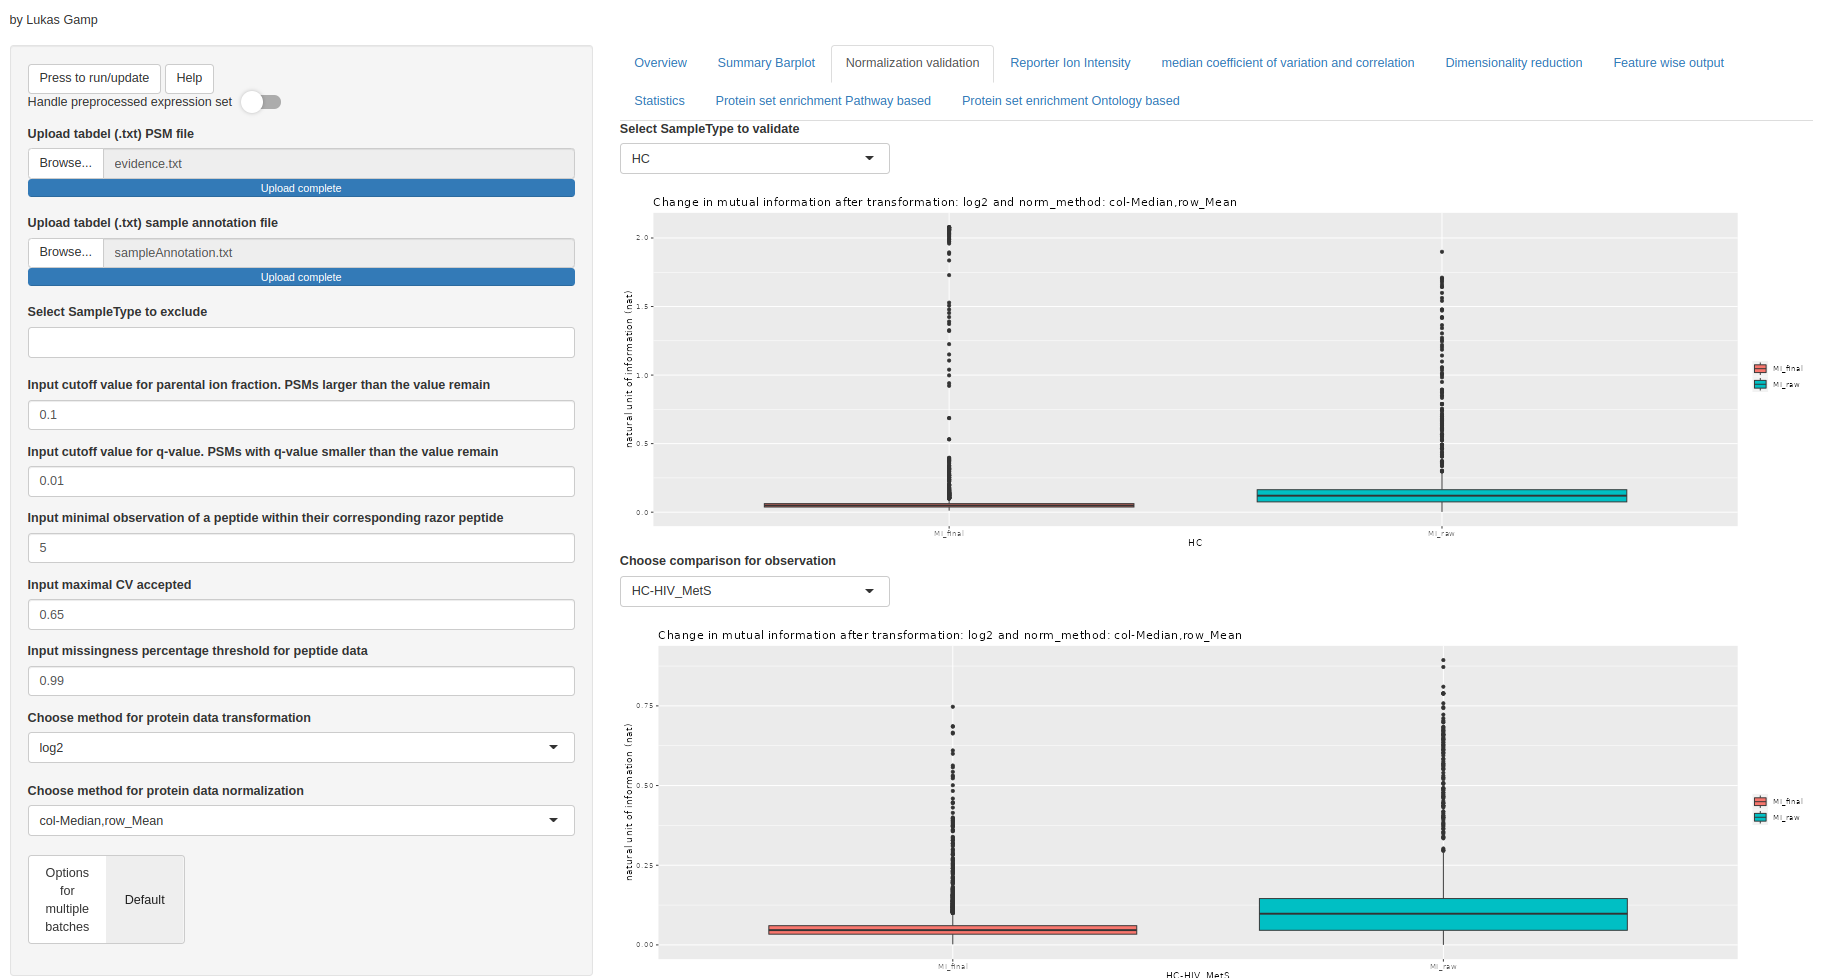
\includegraphics[width=1\linewidth]{screenshots/mutual_info_default} 

}

\caption{Mutual information with default setting}\label{fig:ui_mutual_info_default}
 \endfigure\egroup

After applying logarithmic transformation to the base 2 and performing
column median row mean normalization, the mutual information (MI) within
the healthy control (HC) group's sample type exhibits a reduction
towards the lower edge of the interquartile range (IQR).

MI between the HC group and the sample type corresponding to individuals
with both HIV and metabolic syndrome, the IQR is further reduced and
shifted towards the lower end compared to the MI values observed in the
raw data.

\newpage
\bgroup  \origfigure[H] 

{\centering 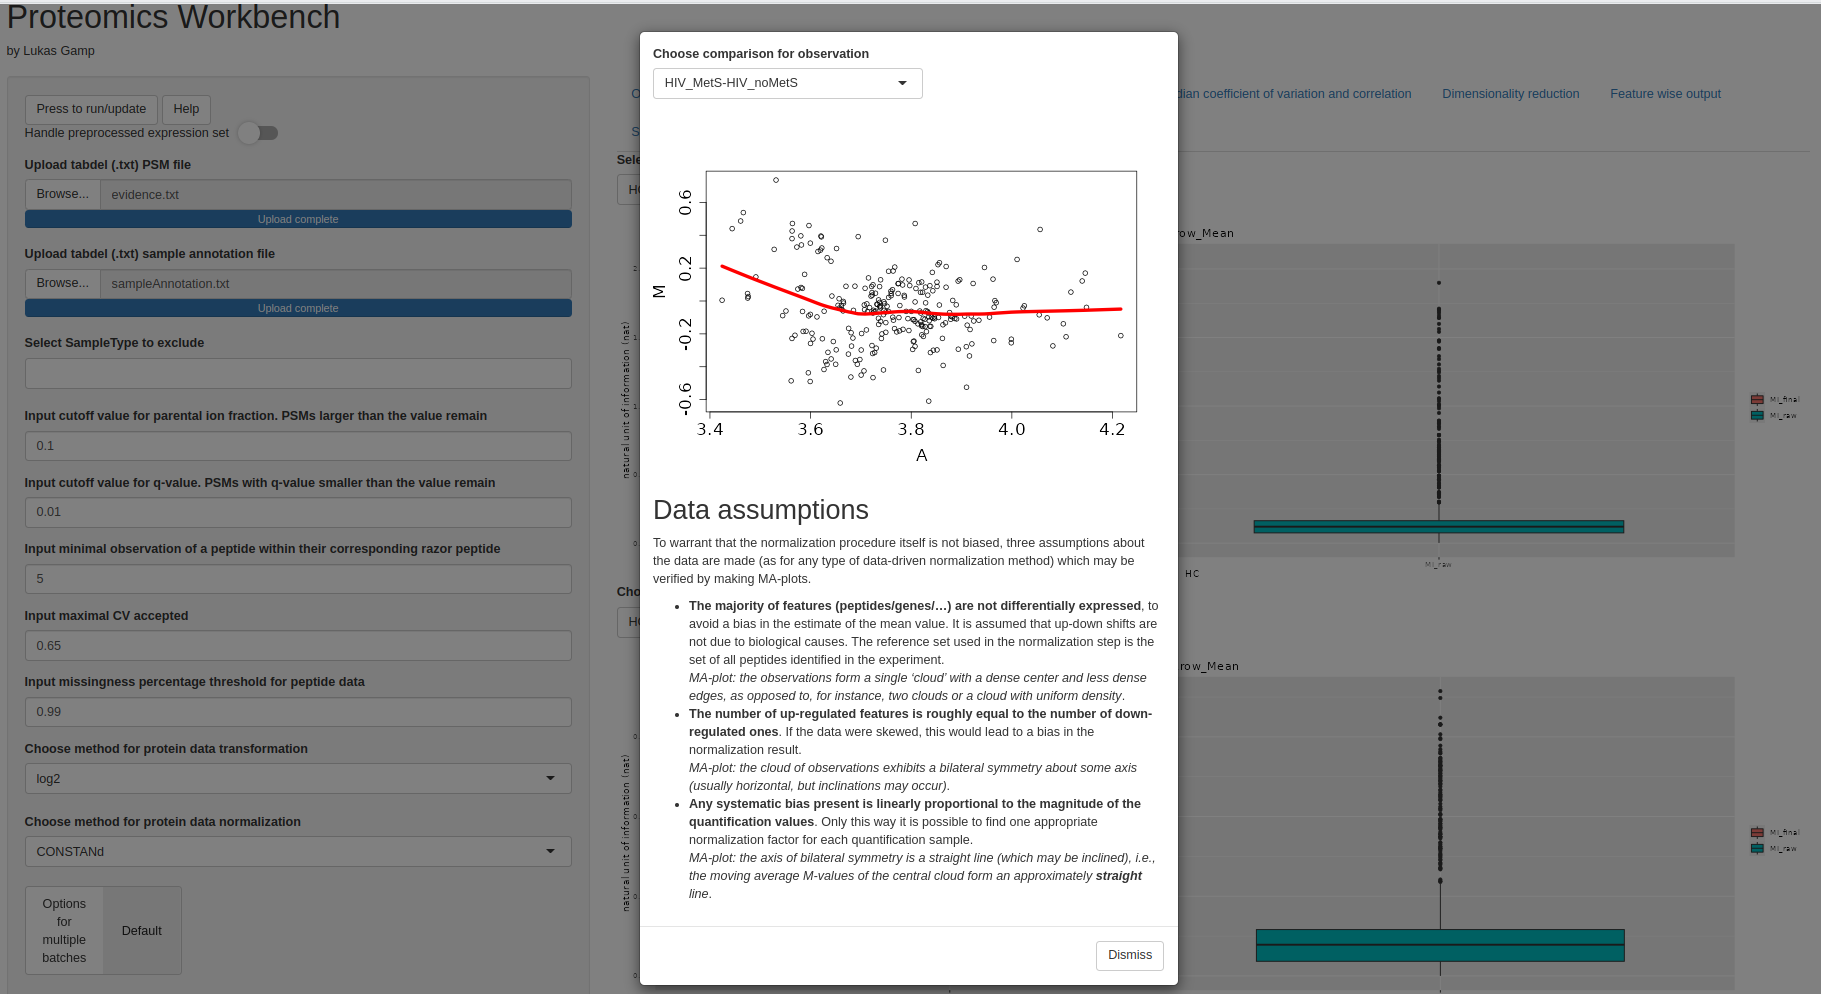
\includegraphics[width=1\linewidth]{screenshots/constand_norm_dependency} 

}

\caption{Popup showing the dependencies for the CONSTANd normalization}\label{fig:ui_constand_norm}
 \endfigure\egroup

\newpage
\bgroup  \origfigure[H] 

{\centering 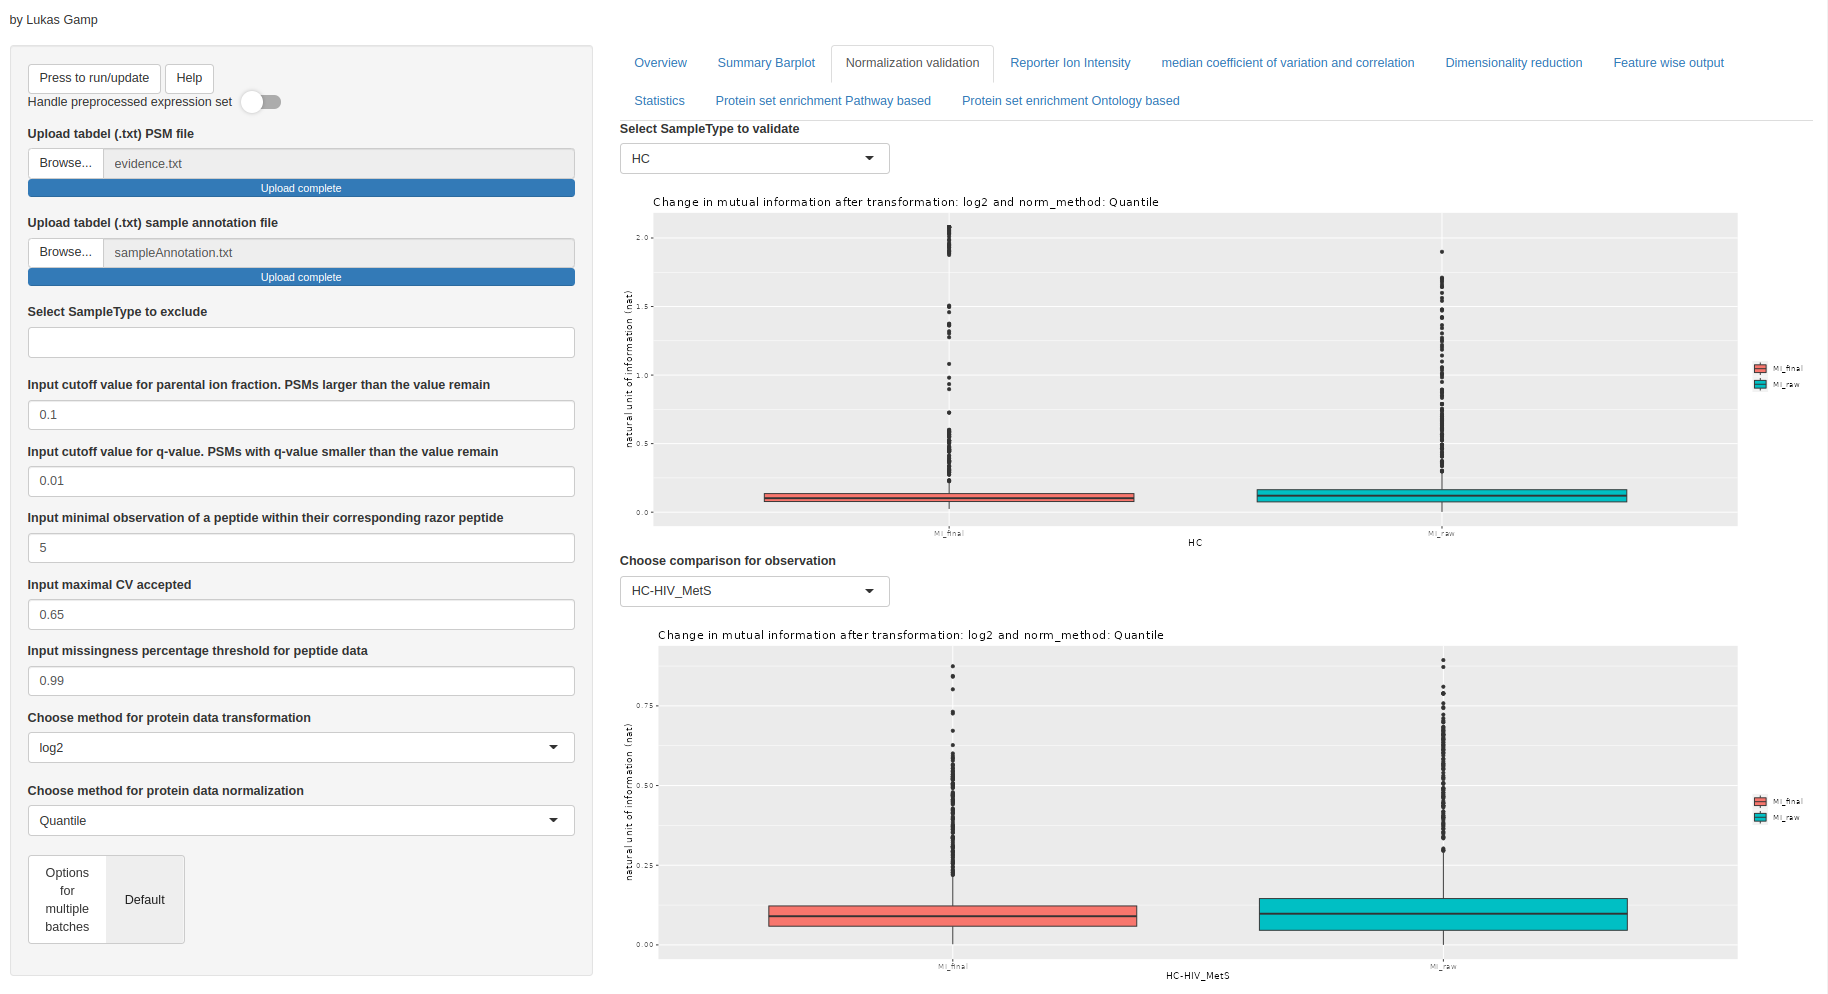
\includegraphics[width=1\linewidth]{screenshots/mutual_info_quant_norm} 

}

\caption{Mutual information with quantile normalization}\label{fig:ui_mutual_info_quant_norm}
 \endfigure\egroup

After performing a logarithmic transformation to the base 2 and quantile
normalization, the mutual information (MI) within the healthy control
(HC) group's sample type exhibits a minor reduction in the interquartile
range (IQR). However, it should be noted that there is an increase in
the number of outliers compared to the raw data.

Observing MI IQR of the HC group with the sample type corresponding to
individuals with both HIV and metabolic syndrome, the reduction in MI
falls within the interquartile range of the raw data MI. Additionally,
the median remains close to unaffected, indicating that the overall
central tendency of the MI values is relatively preserved.

\newpage
\bgroup  \origfigure[H] 

{\centering 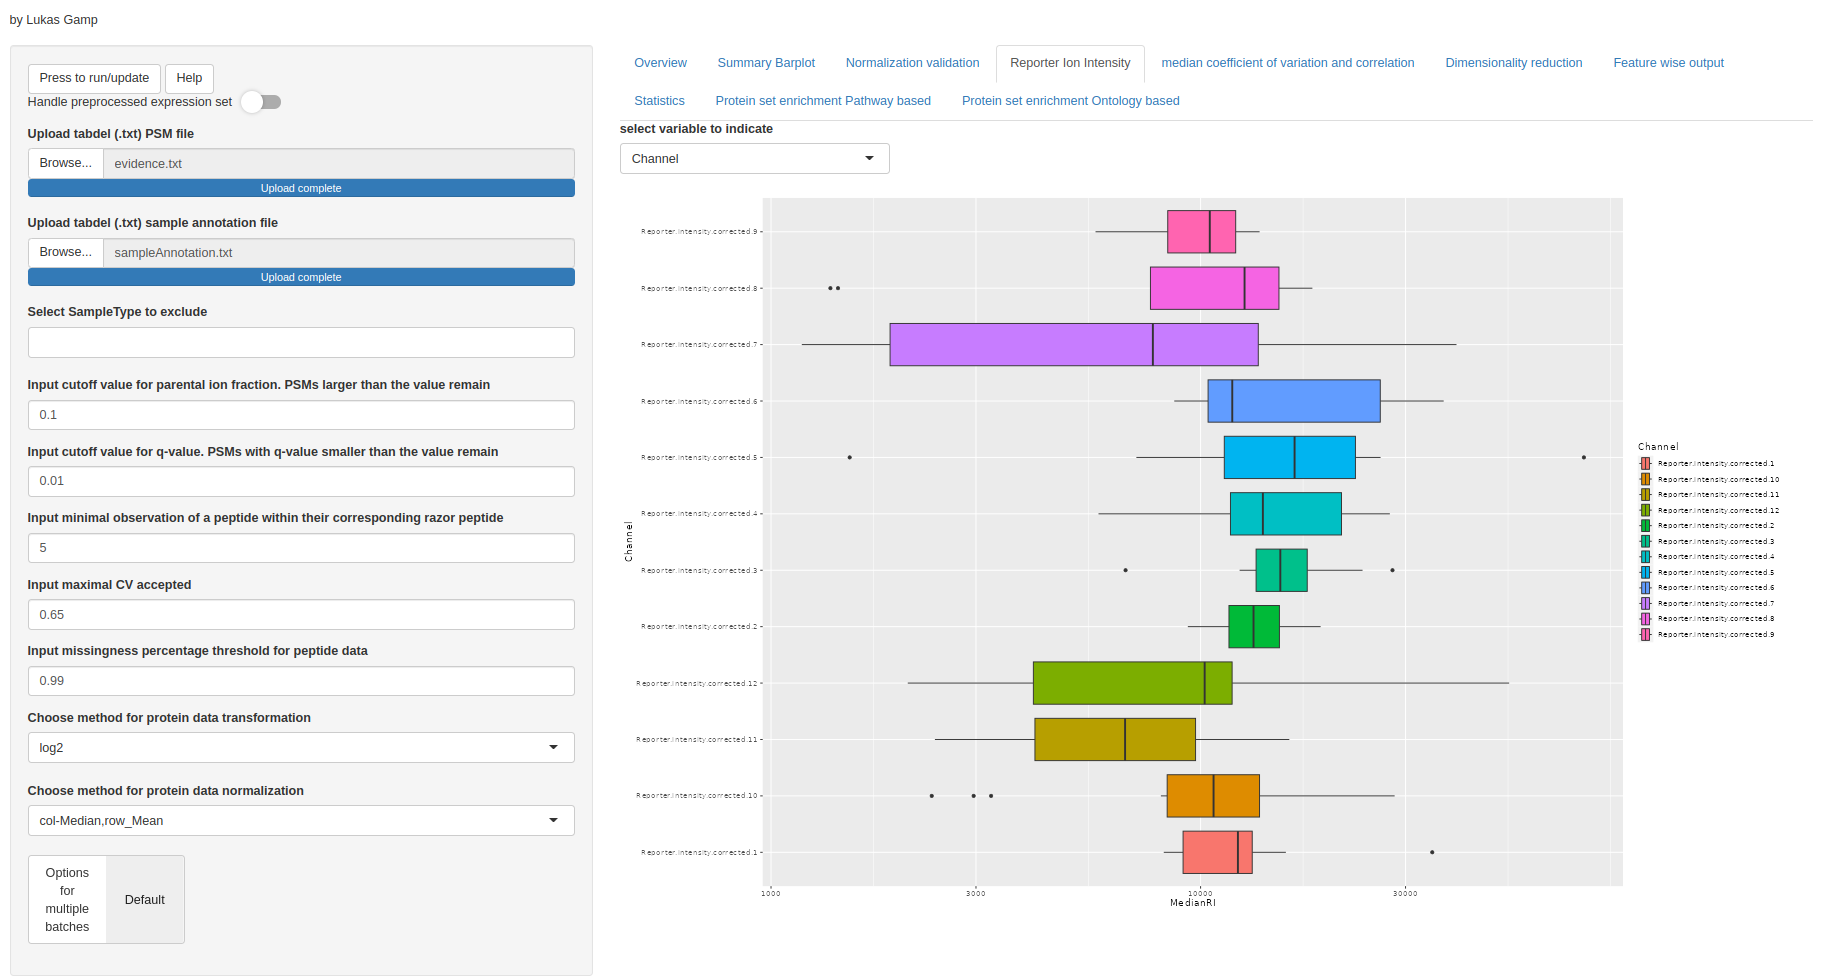
\includegraphics[width=1\linewidth]{screenshots/RI_channel_default} 

}

\caption{Reporter ion intensity with selection on channel. The selected factor will be highlighted and indicated in the legend.}\label{fig:ui_RI_channel_default}
 \endfigure\egroup

When comparing the median reporter ion intensities across channels, no
systematic bias is observed. However, it is worth noting that channel 7
exhibits a wide range of values spanning an order of magnitude. This
comparison is crucial since the three sample types consistently occupy
the same channels in every run, making the visualization an important
aspect of the analysis. Despite the wide range of values in channel 7,
there is still overlap in the interquartile ranges (IQR) across the
majority of samples.

\newpage
\bgroup  \origfigure[H] 

{\centering 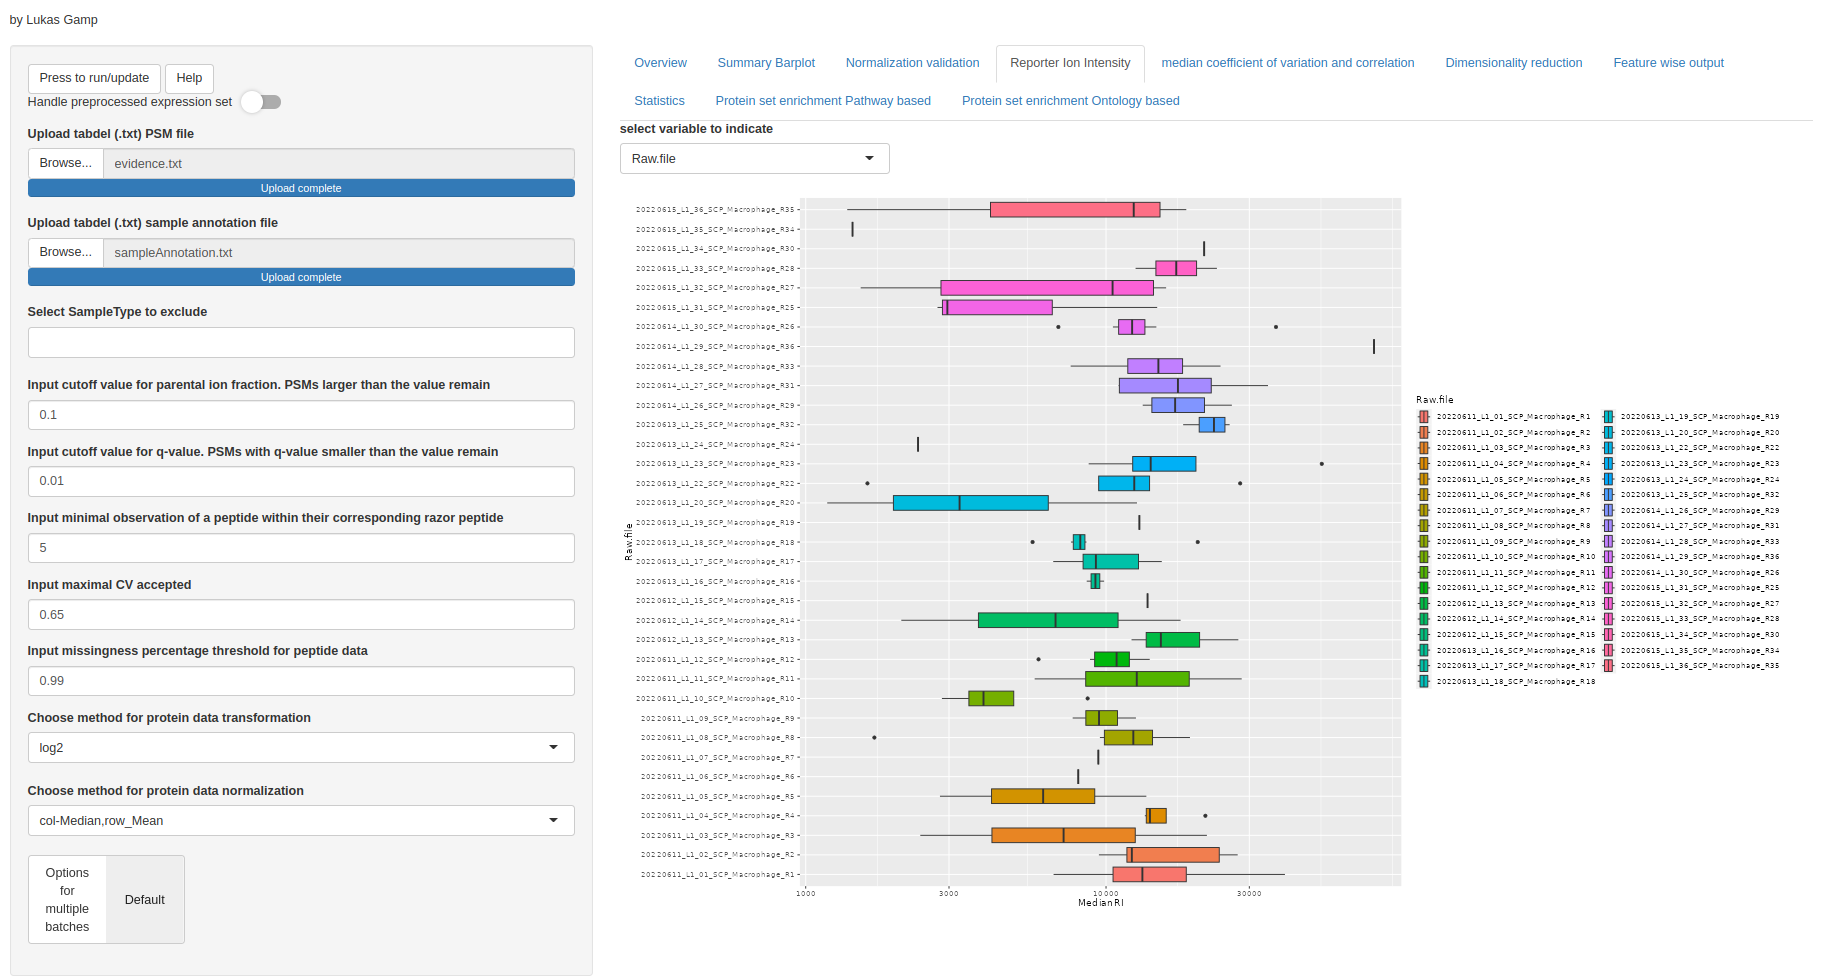
\includegraphics[width=1\linewidth]{screenshots/RI_file_default} 

}

\caption{Reporter ion intensity with selection on file}\label{fig:ui_RI_file_default}
 \endfigure\egroup

Comparing the median reporter ion intensities with a focus on the batch
(=Raw.file), it becomes evident that there are significant changes in
signal that need to be taken into account in further analysis. After
applying quality control measures, several values have been lost due to
cutoffs in parameters such as parental ion fraction (PIF), q-value,
coefficient of variation, and missingness of peptide data.

For dimensionality reduction, the user has the option to choose the
batch correction method ComBat \citep{Leek2012} in the side panel.
However, this option is not set as the default choice. Instead, the
conservative approach is followed, where the batch factor is included in
the statistical module to account for any potential batch effects that
may influence the results.

\newpage
\bgroup  \origfigure[H] 

{\centering 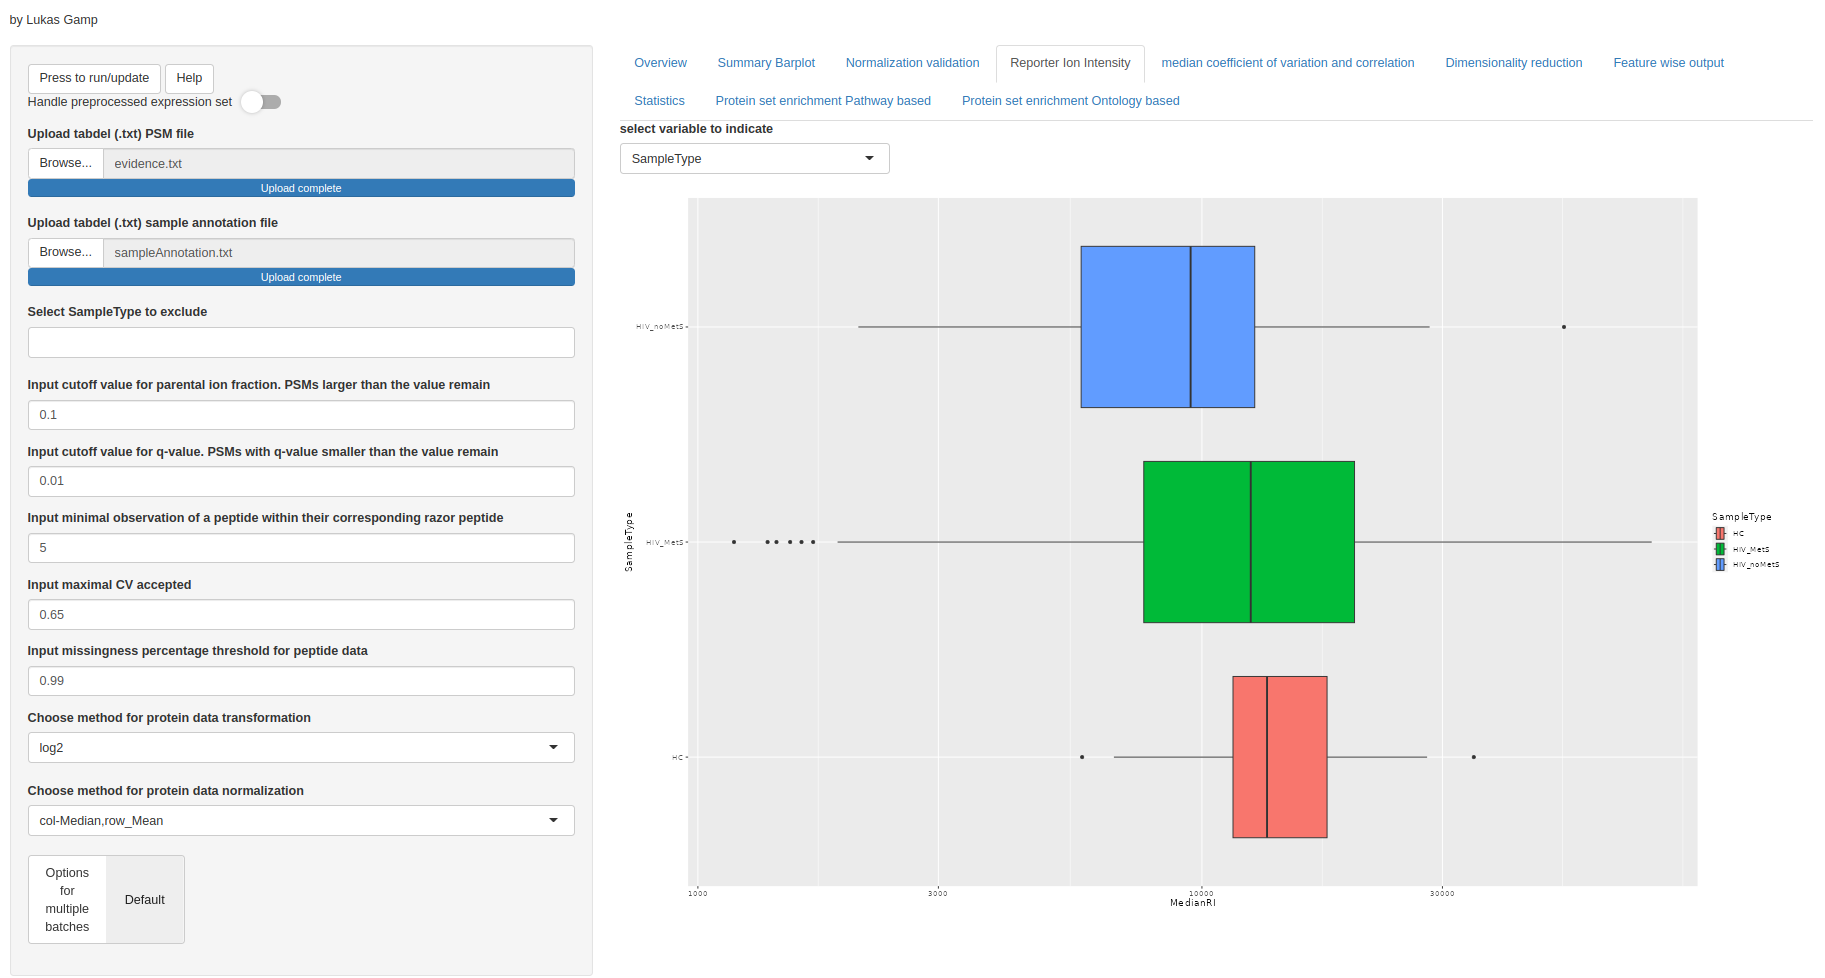
\includegraphics[width=1\linewidth]{screenshots/RI_st_default} 

}

\caption{Reporter ion intensity with selection on sampletype}\label{fig:ui_RI_st_default}
 \endfigure\egroup

The sample type does not appear to have an impact on the median reporter
ion intensities, as suggested by the overlapping interquartile ranges
(IQRs). Nevertheless, the HIV group with metabolic syndrome displays a
broader range of values spanning tenfold in arbitrary units.

\newpage
\bgroup  \origfigure[H] 

{\centering 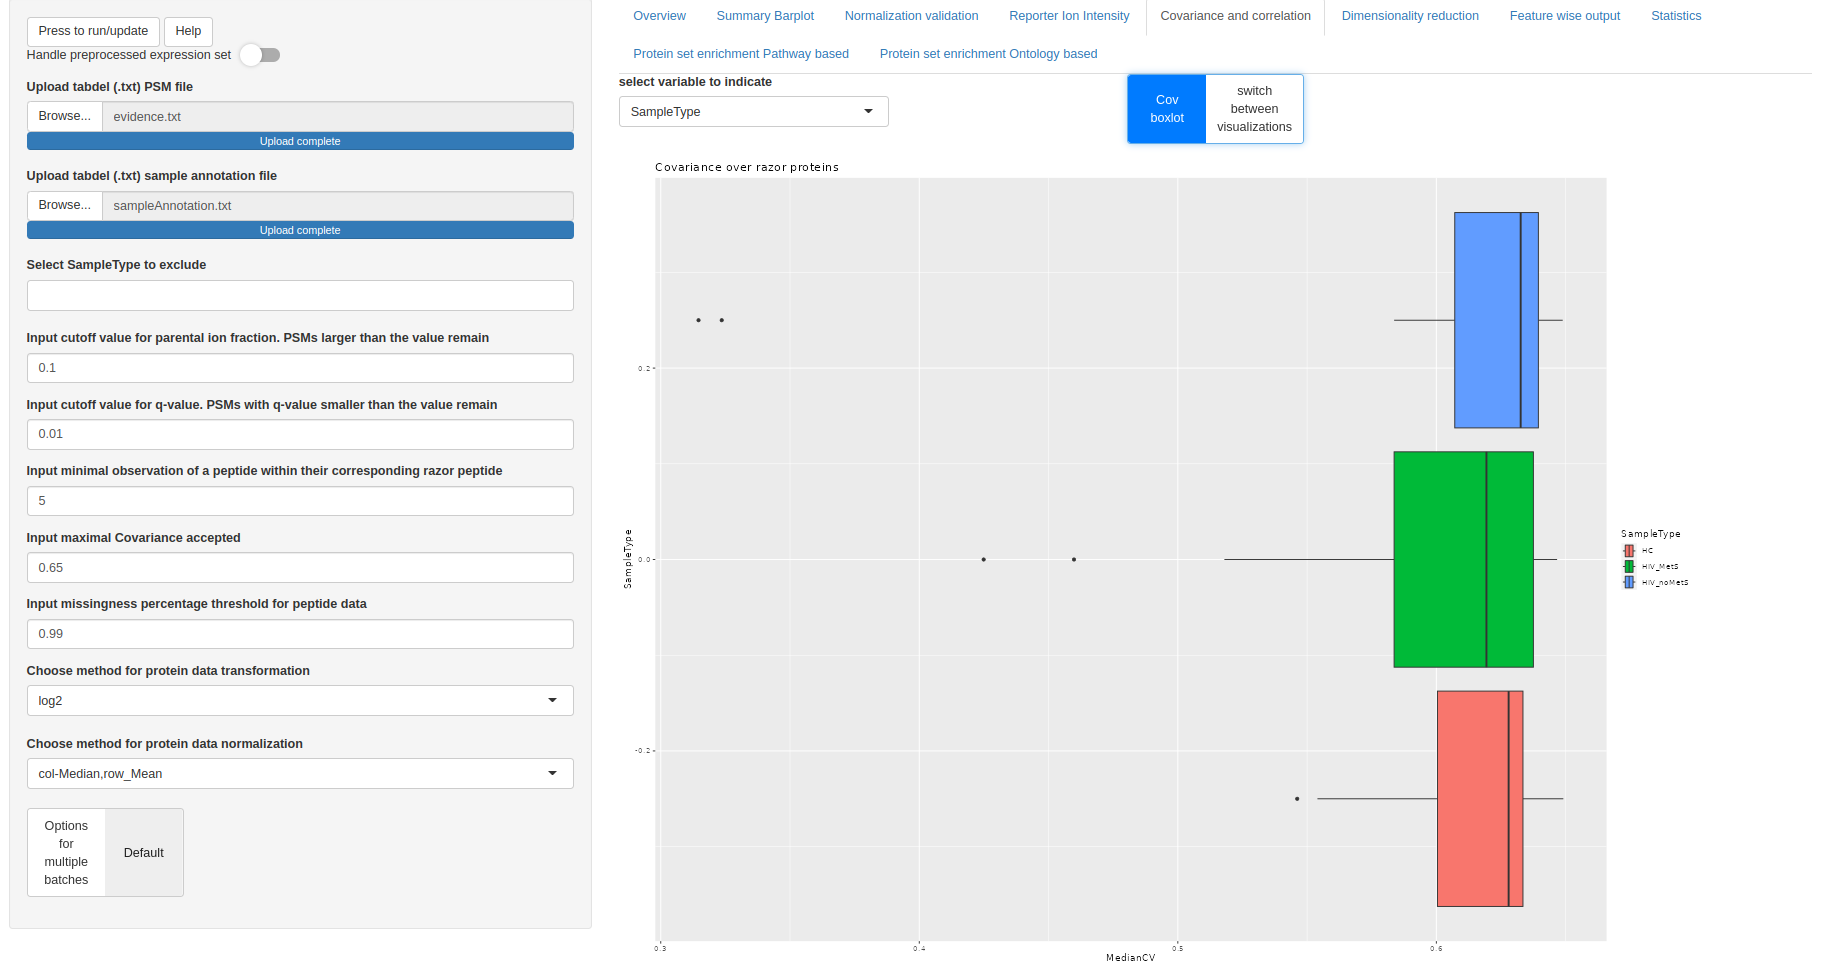
\includegraphics[width=1\linewidth]{screenshots/cv_st_default} 

}

\caption{Median covariance of razor proteins with selection on sampletype}\label{fig:ui_cv_st_default}
 \endfigure\egroup

A cutoff value of 0.65 for the coefficient of variation (CV) of razor
proteins as shown in the SCoPE2 publication \citep{Specht2021}
demonstrates a satisfactory fit to the data. The minimum number of
observations determines the threshold for considering a razor protein
ambiguous, based on the number of matching peptides. In this case, the
reference publication set the threshold at 5 observations.

The interquartile ranges (IQRs) remained unchanged by this cutoff. The
sample type did not influence the CV of razor proteins. Boxplots
illustrate that the values are distributed similarly, as indicated by
the overlapping IQRs.

\newpage
\bgroup  \origfigure[H] 

{\centering 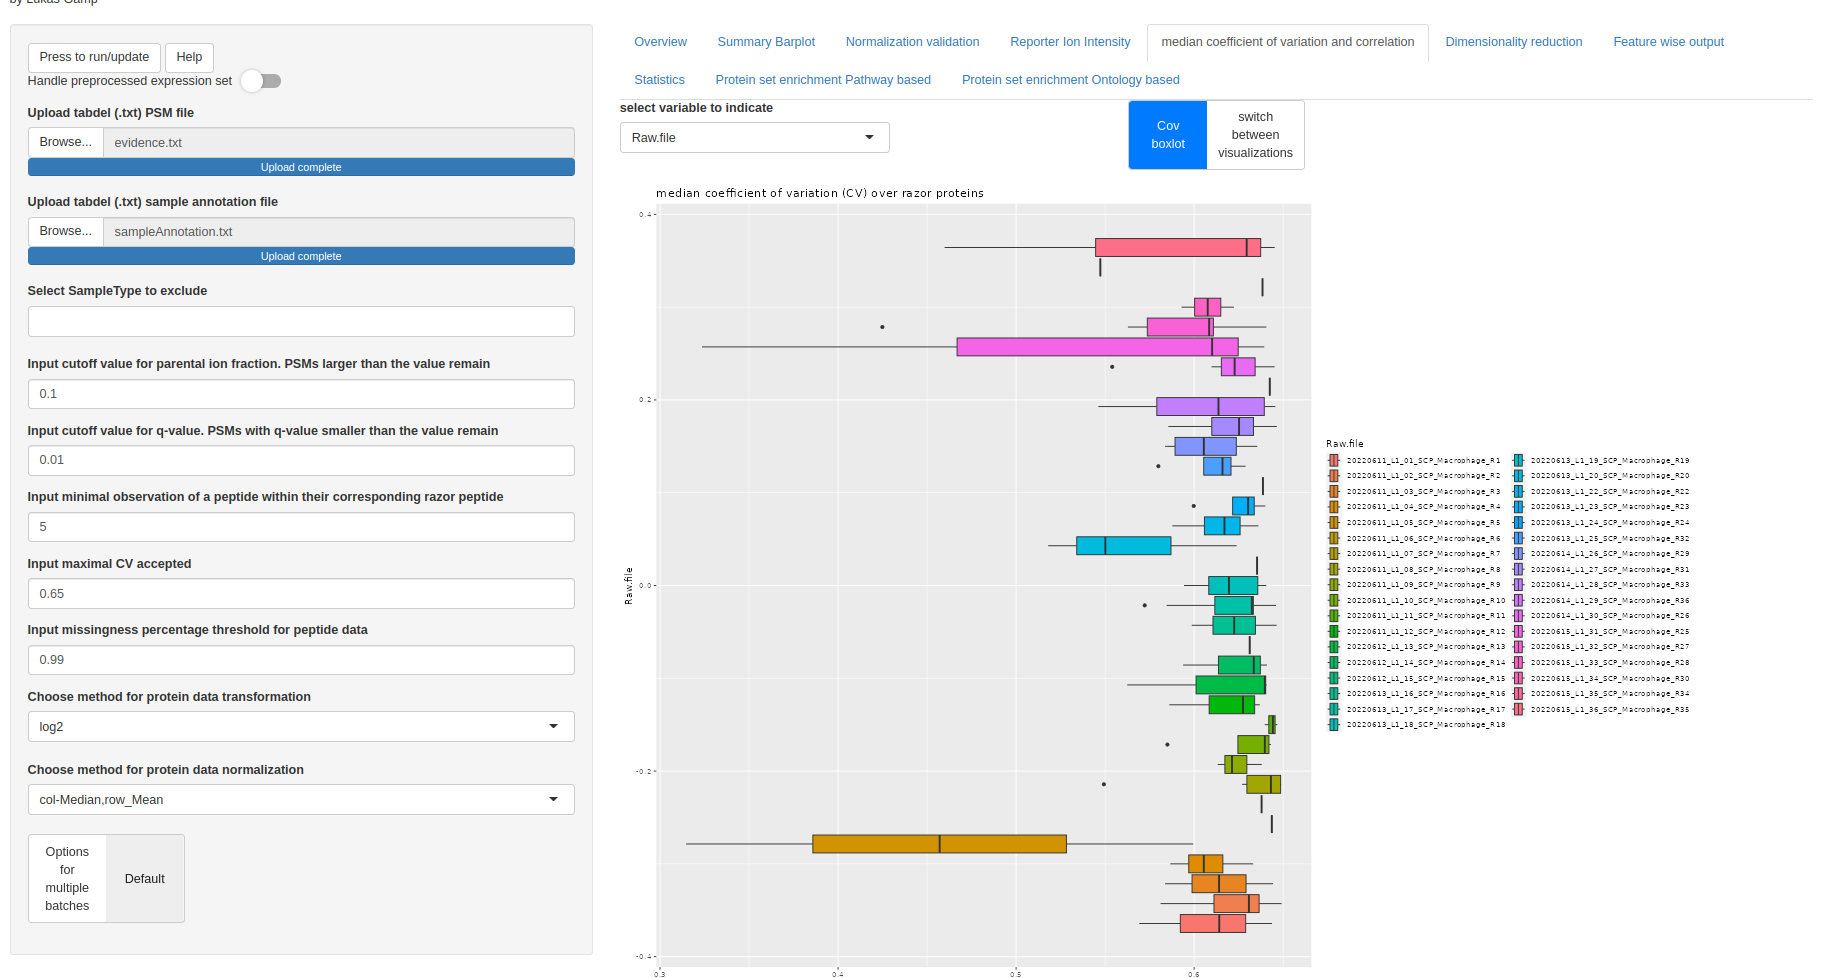
\includegraphics[width=1\linewidth]{screenshots/cv_rawfile_default} 

}

\caption{Median coefficient of variation (CV) of leading razor proteins per cell with selection on Raw.file}\label{fig:ui_cv_rawfile_default}
 \endfigure\egroup

The plot illustrates that certain batches (=raw files) exhibit a higher
number of distinct matches compared to others, as indicated by a thin
line depicting low density. Most interquartile ranges (IQRs) overlap,
suggesting similarity among the majority of batches. However, specific
batches display a lower IQR in median CV across razor protein peptides,
indicating distinct matches.

\newpage
\bgroup  \origfigure[H] 

{\centering 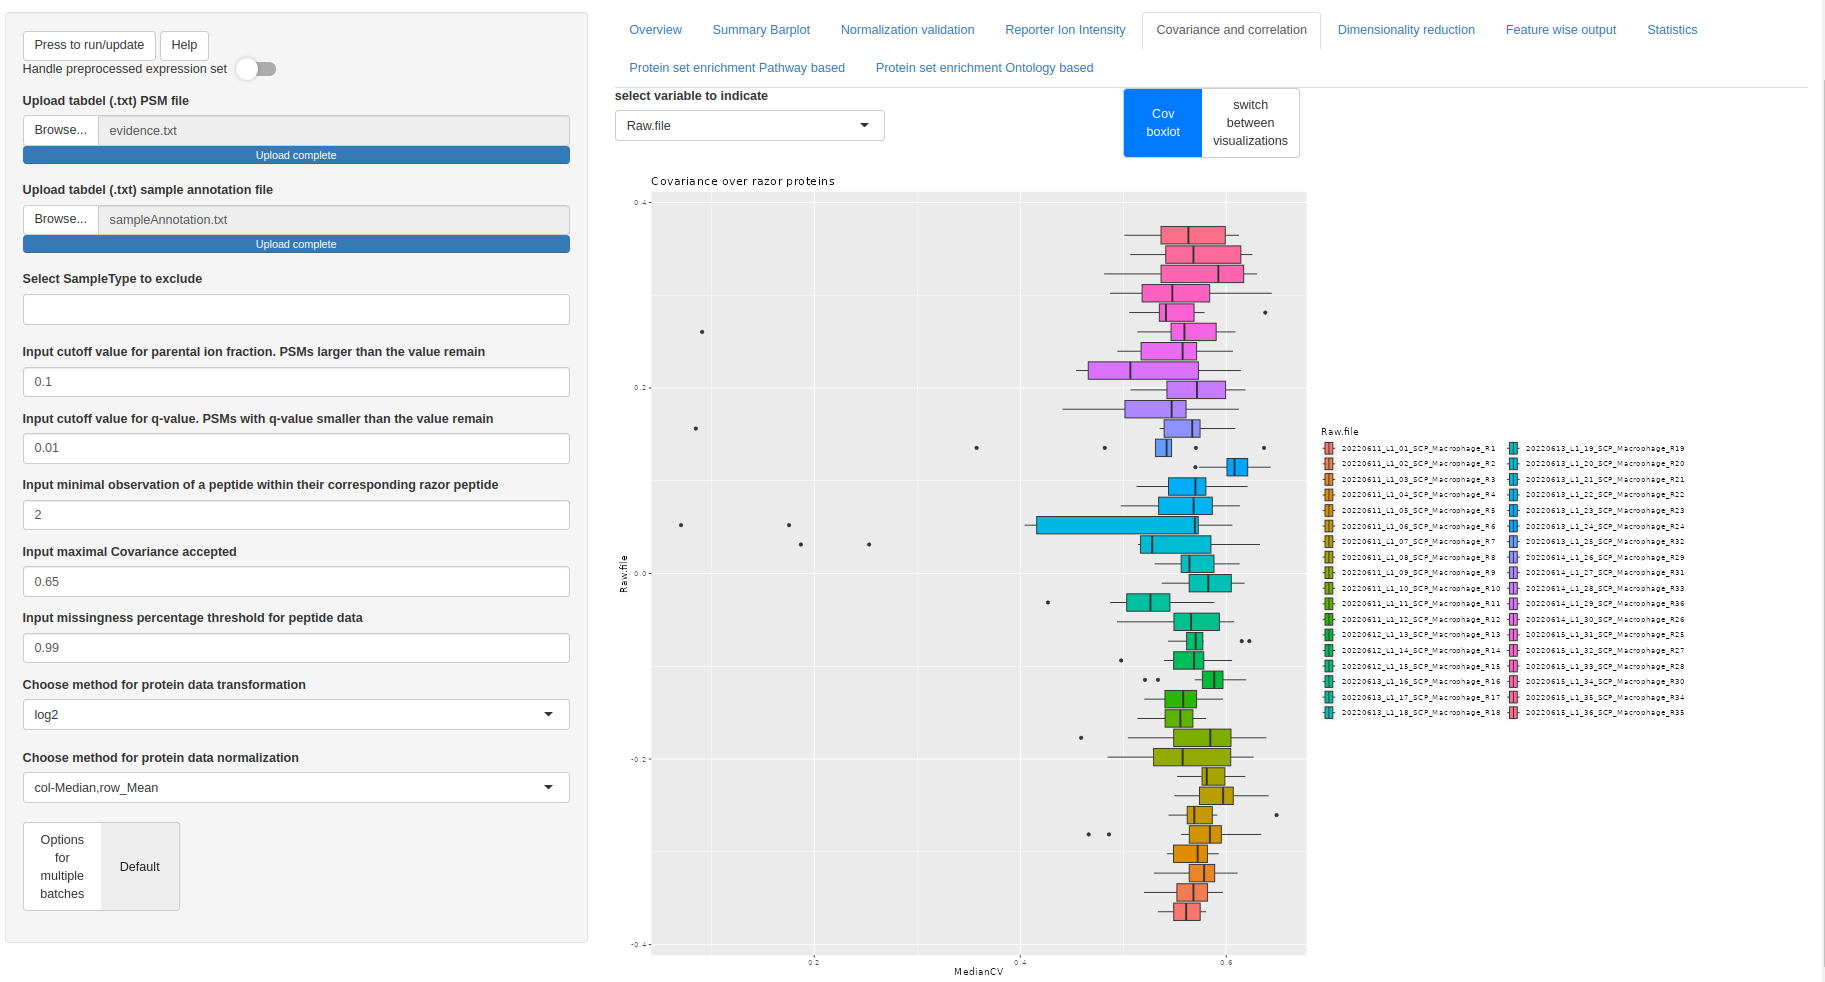
\includegraphics[width=1\linewidth]{screenshots/cv_rawfile_nobs2} 

}

\caption{Median coefficient of variation (CV) of leading razor proteins calculated for 2  observations per cell, with selection on Raw.file}\label{fig:ui_cv_rawfile_nobs2}
 \endfigure\egroup

By setting the number of observations to 2, the distributions become
more equalized. Additionally, batches that initially exhibited a
decreased coefficient of variation (CV) tend to inflate towards the
threshold.

\newpage
\bgroup  \origfigure[H] 

{\centering 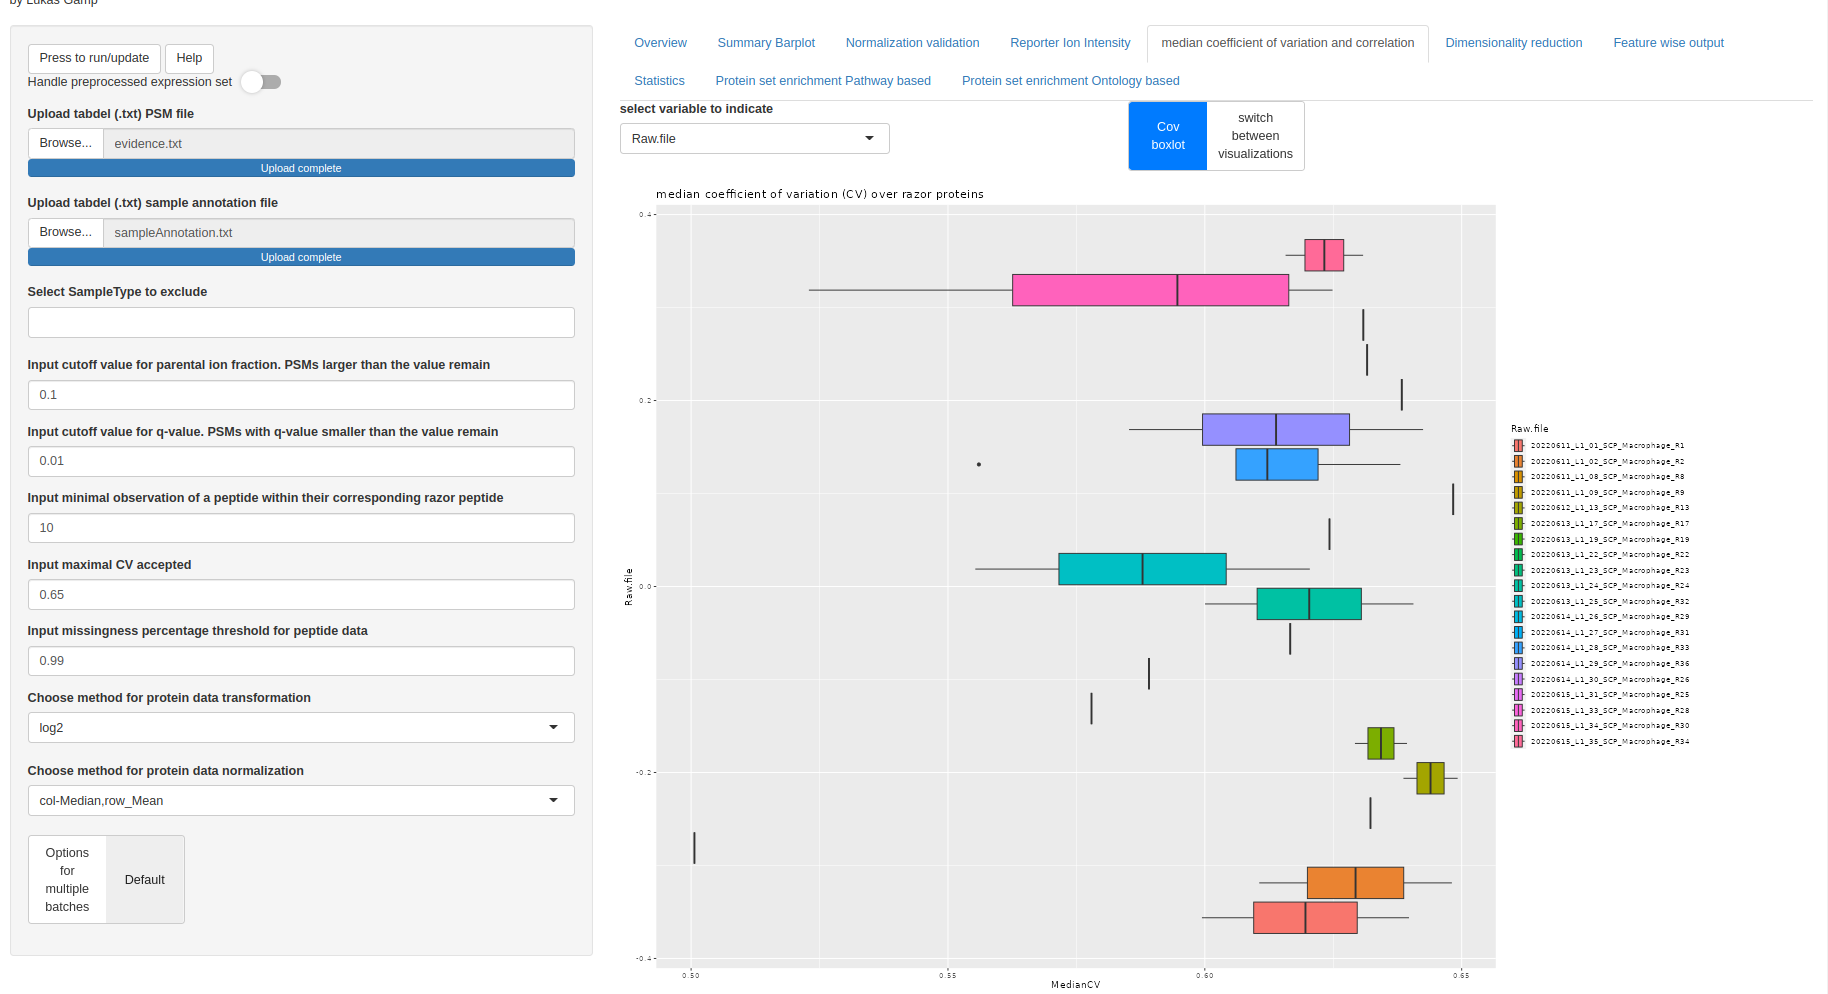
\includegraphics[width=1\linewidth]{screenshots/cv_rawfile_nobs10} 

}

\caption{Median coefficient of variation (CV) of leading razor proteins calculated for 10 observations per cell, with selection on Raw.file}\label{fig:ui_cv_rawfile_nobs10}
 \endfigure\egroup

When the minimum number of observations for ambiguous peptides is set to
10, the distribution of medians across channels shows a decrease in
density. This can be attributed to the rare occurrence of 10 unique
peptides matching to the same protein, which is not commonly observed in
the dataset.

\newpage
\bgroup  \origfigure[H] 

{\centering 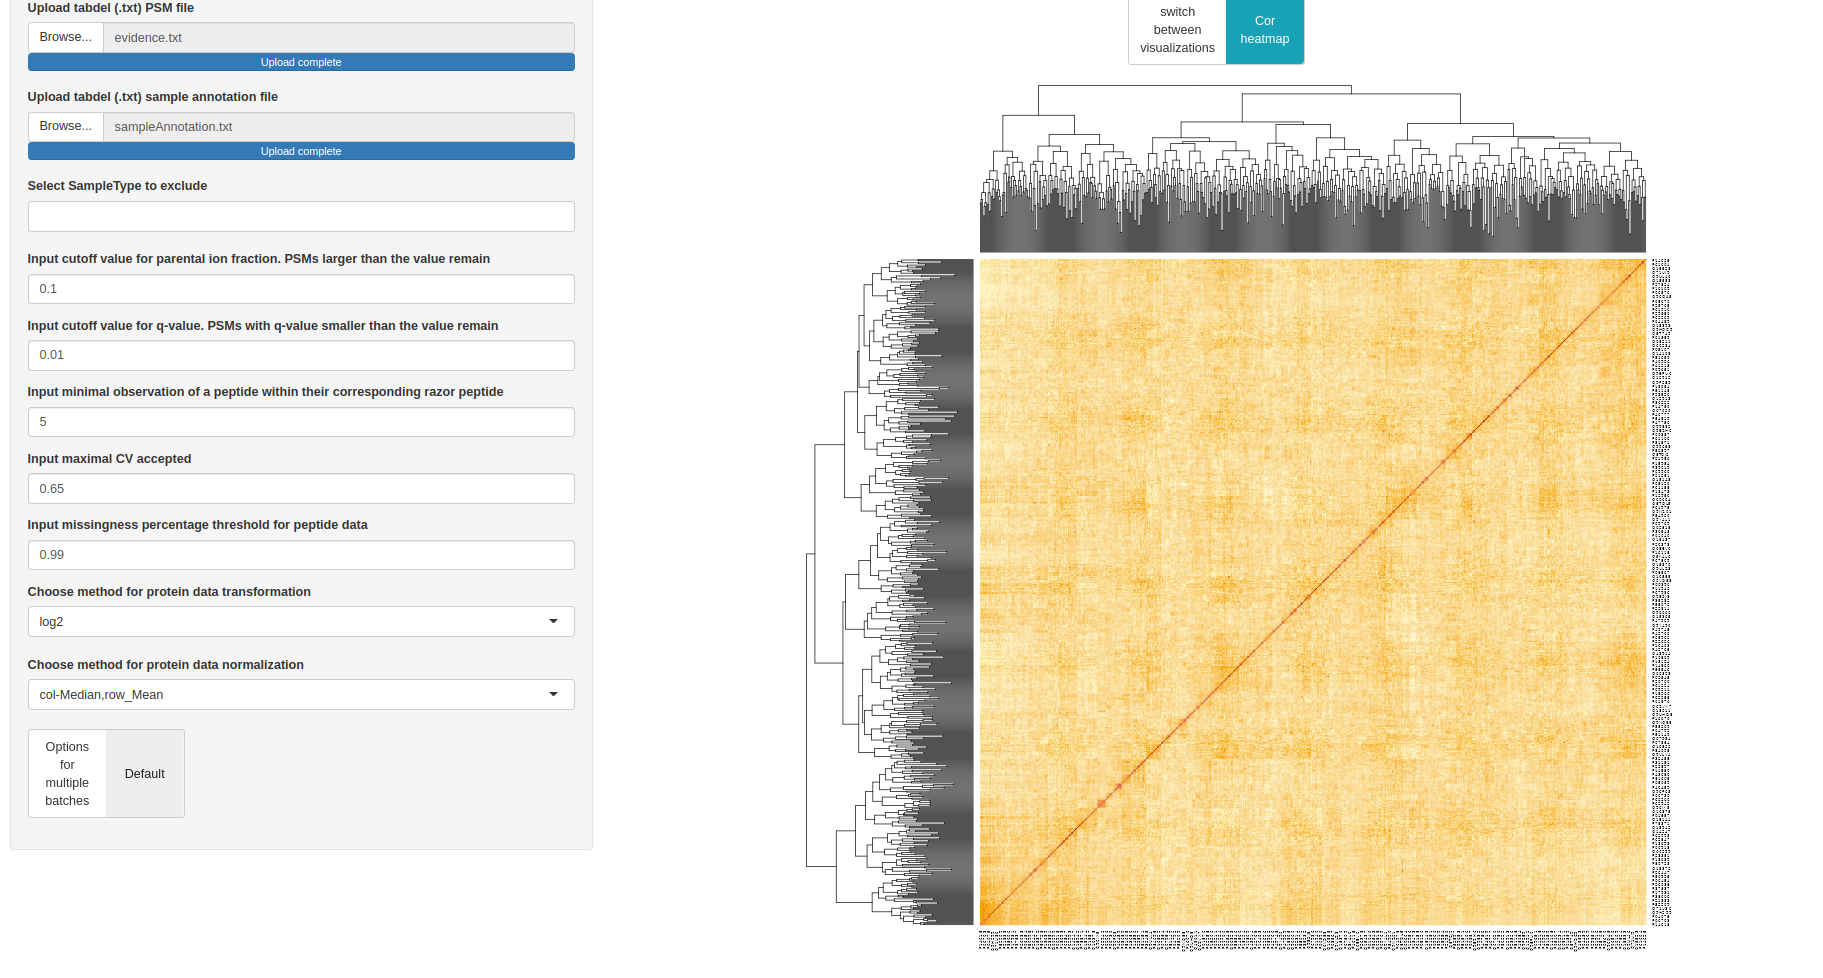
\includegraphics[width=1\linewidth]{screenshots/heatmap} 

}

\caption{Correlation heatmap}\label{fig:ui_heatmap}
 \endfigure\egroup

The heatmap reveals the Pearson pairwise correlation coefficients
between all proteins. The dendrogram indicates that there are two main
protein clusters, with one of the clusters showing further
sub-clustering, indicating a strong relationship among the proteins in
the sub groups. However, the other cluster, consisting of individual
proteins, shows weaker correlations, leading to a more intricate
branching pattern in the dendrogram.

\newpage
\bgroup  \origfigure[H] 

{\centering 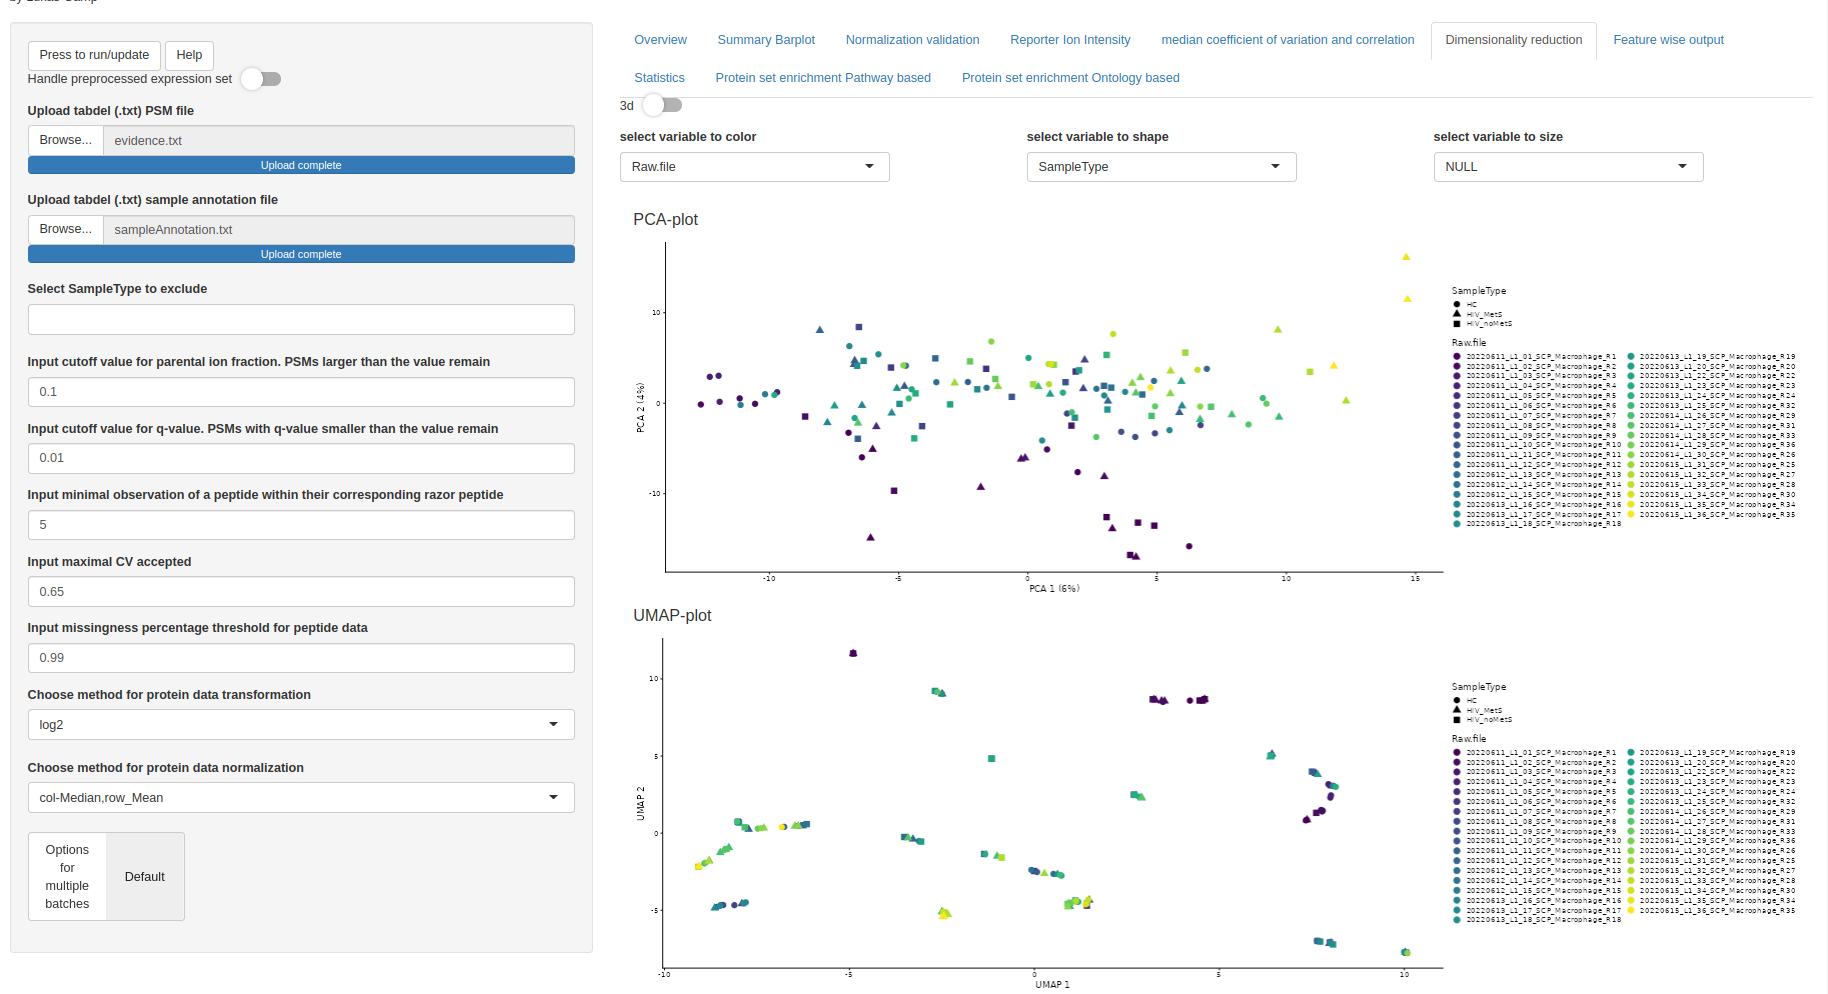
\includegraphics[width=1\linewidth]{screenshots/dim_red_default} 

}

\caption{Dimensionality reduction analysis depicting sample types (indicated by shape) and raw files (indicated by color). Top: principle component analysis (PCA). Lower: Uniform Manifold Approximation and Projection (UMAP)}\label{fig:ui_dim_red_default}
 \endfigure\egroup

In both the Principal Component Analysis (PCA) plot and the Uniform
Manifold Approximation and Projection (UMAP) plot, the second component
is plotted against the first component. Surprisingly, neither
visualization reveals any discernible clustering patterns based on
sample type or batch. For the k-nearest neighbor descent algorithm
(NN-descent) employed in the UMAP, first a default value of k=3 was
selected.

\newpage
\bgroup  \origfigure[H] 

{\centering 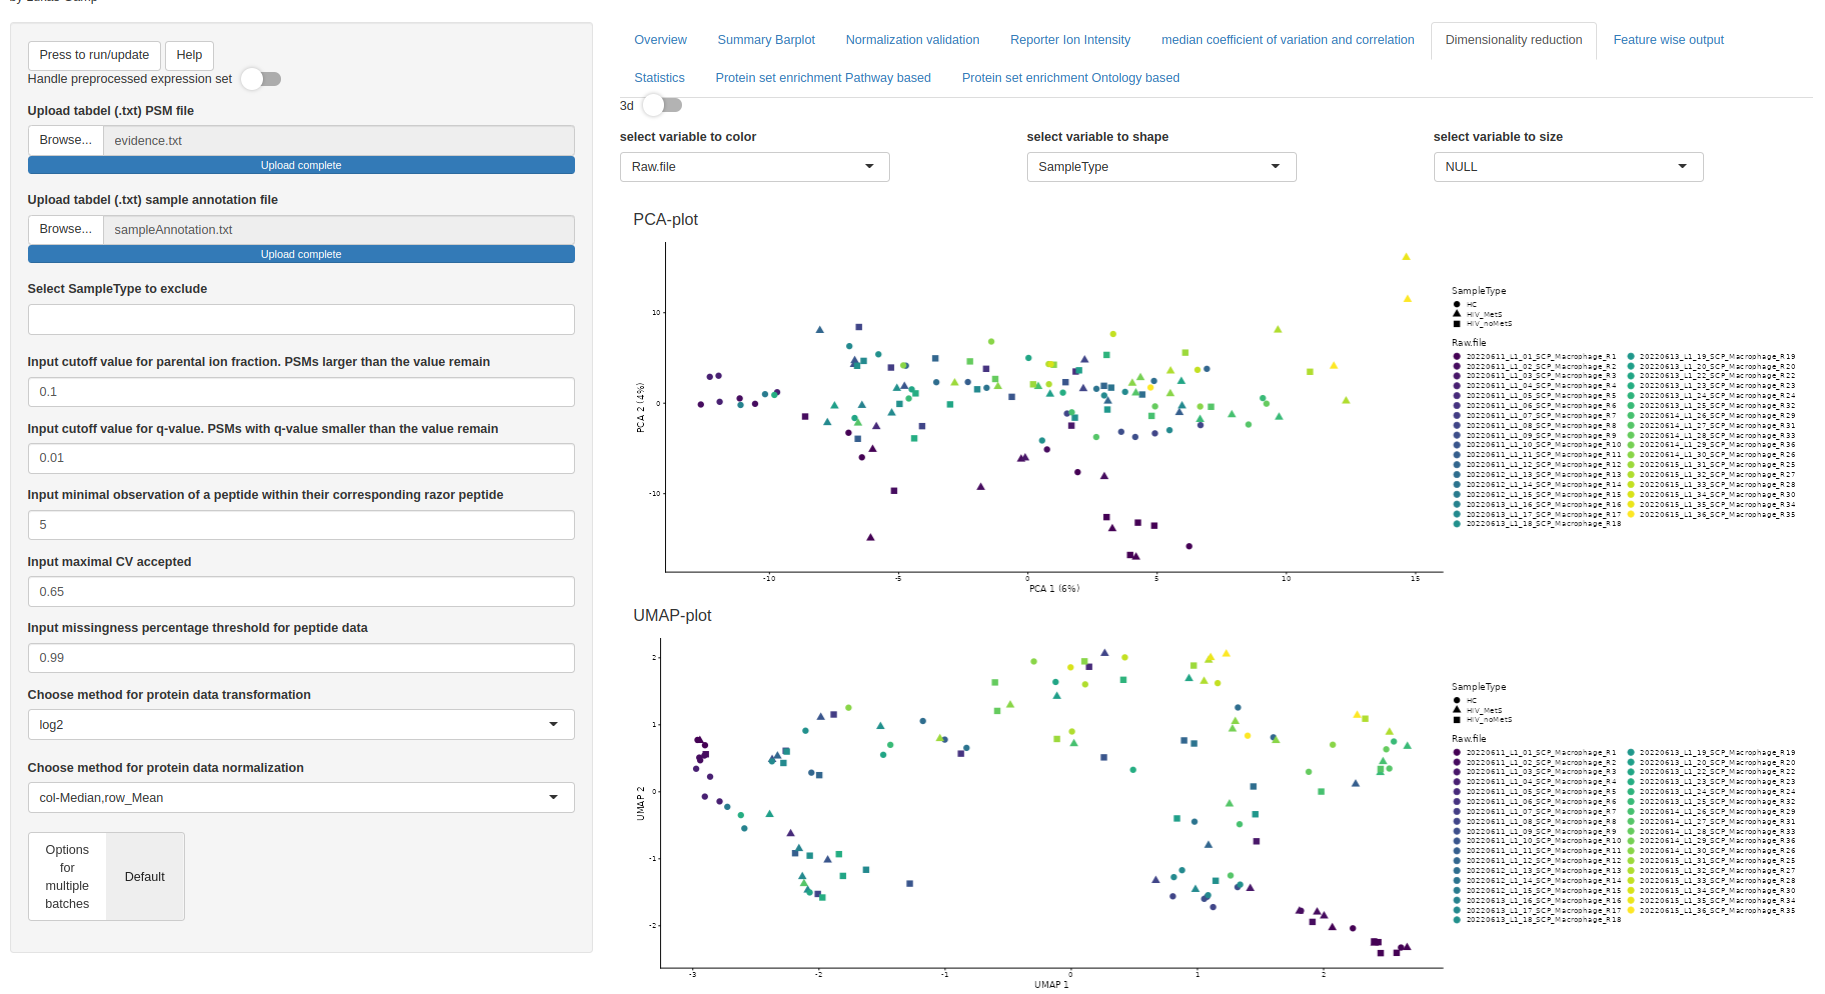
\includegraphics[width=1\linewidth]{screenshots/dim_red_changed_k} 

}

\caption{Dimensionality reduction analysis showcasing sample types (represented by shape) and raw files (represented by color). Top: Principal Component Analysis (PCA). Bottom: Uniform Manifold Approximation and Projection (UMAP). For the UMAP visualization, the k value for the NN-descent algorithm was modified to 15.}\label{fig:ui_dim_red_changed_k}
 \endfigure\egroup

The second figure of the Principal Component Analysis (PCA) plot and the
Uniform Manifold Approximation and Projection (UMAP), both displaying
the second component against the first. Surprisingly, neither
visualization reveals any discernible clustering patterns based on
sample type or batch information. To enhance the resolution and capture
more intricate patterns, the k-nearest neighbor descent algorithm
(NN-descent) was adjusted, with a value of K set to 15. While the
resulting plot exhibits improved detail, the underlying biological
context or background remains elusive and does not emerge in the visual
representation.

\newpage
\bgroup  \origfigure[H] 

{\centering 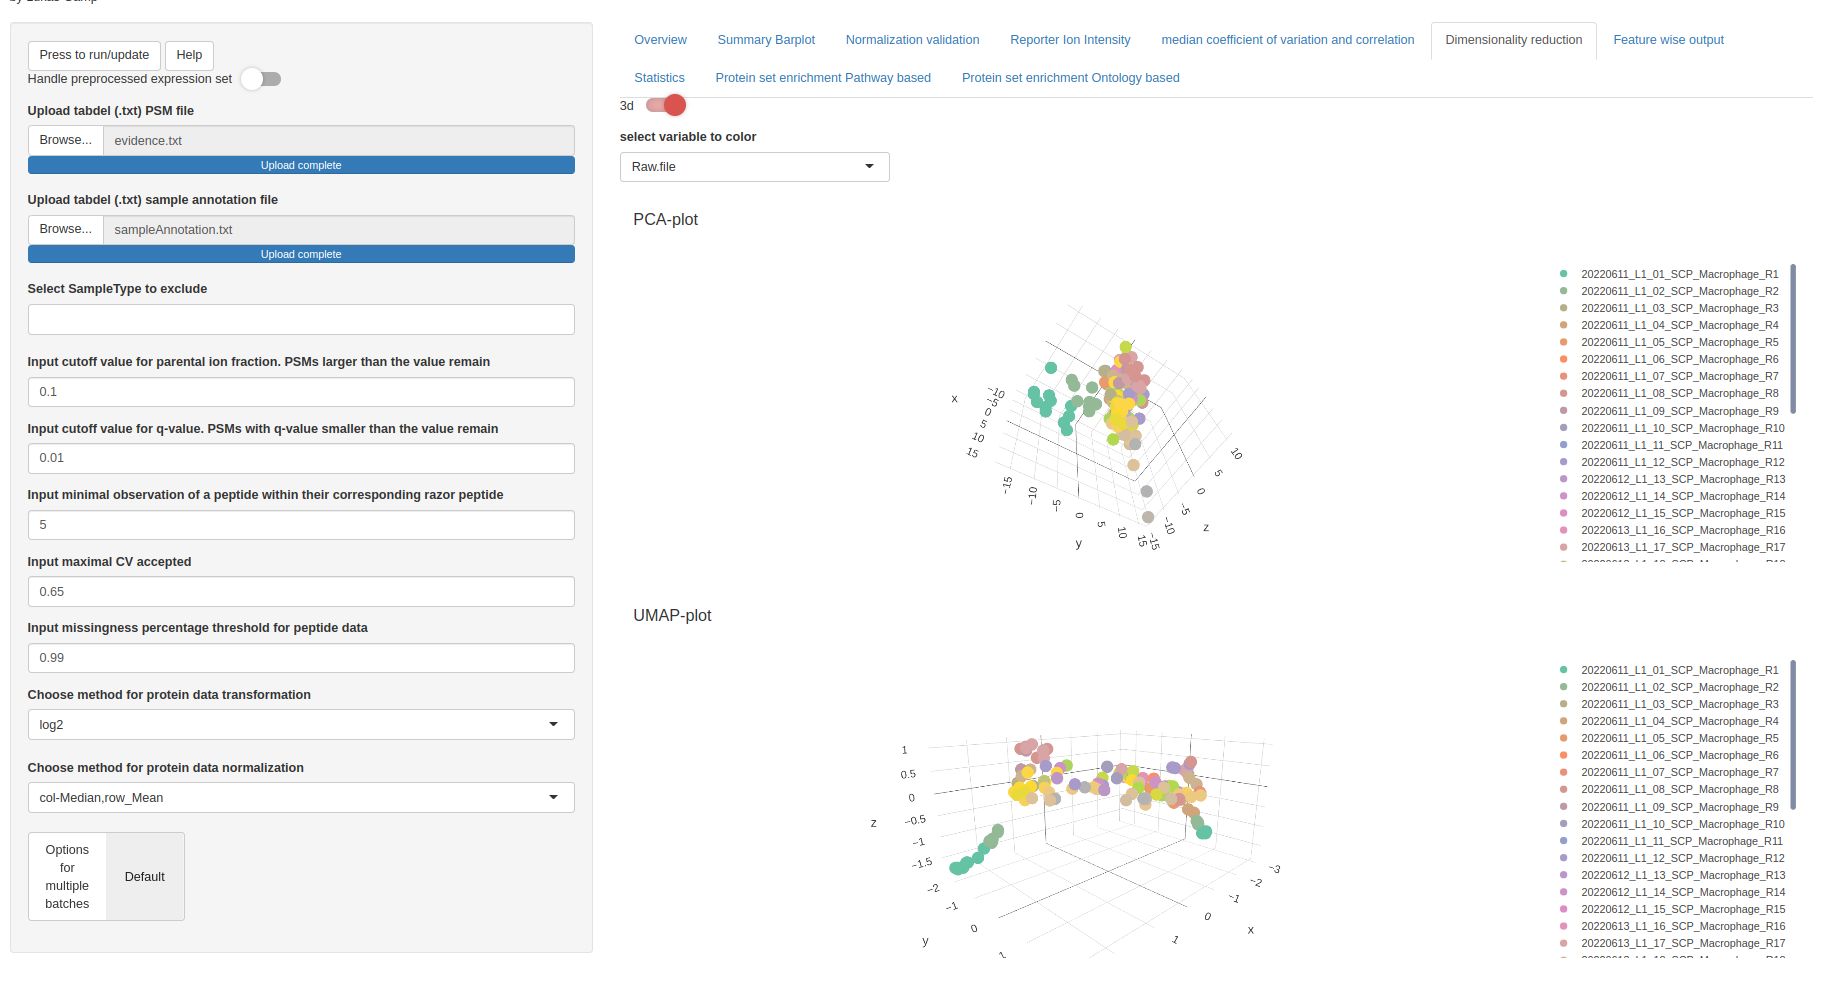
\includegraphics[width=1\linewidth]{screenshots/dim_red_3d} 

}

\caption{3D visualization of dimensionality reduction analysis showcasing sample types (represented by shape) and raw files (represented by color). Top: Principal Component Analysis (PCA). Bottom: Uniform Manifold Approximation and Projection (UMAP)}\label{fig:ui_dim_red_c3d}
 \endfigure\egroup

In the 3D visualization, a subtle clustering pattern can be observed for
the first two batches. Upon switching to the indicator sample type in
the 3D visualization, no clustering can be observed whatsoever. This
suggests that the variance in the data set is not attributed to sample
type or batch, reinforcing the notion that other factors could
contribute to the observed variability.

\newpage
\bgroup  \origfigure[H] 

{\centering 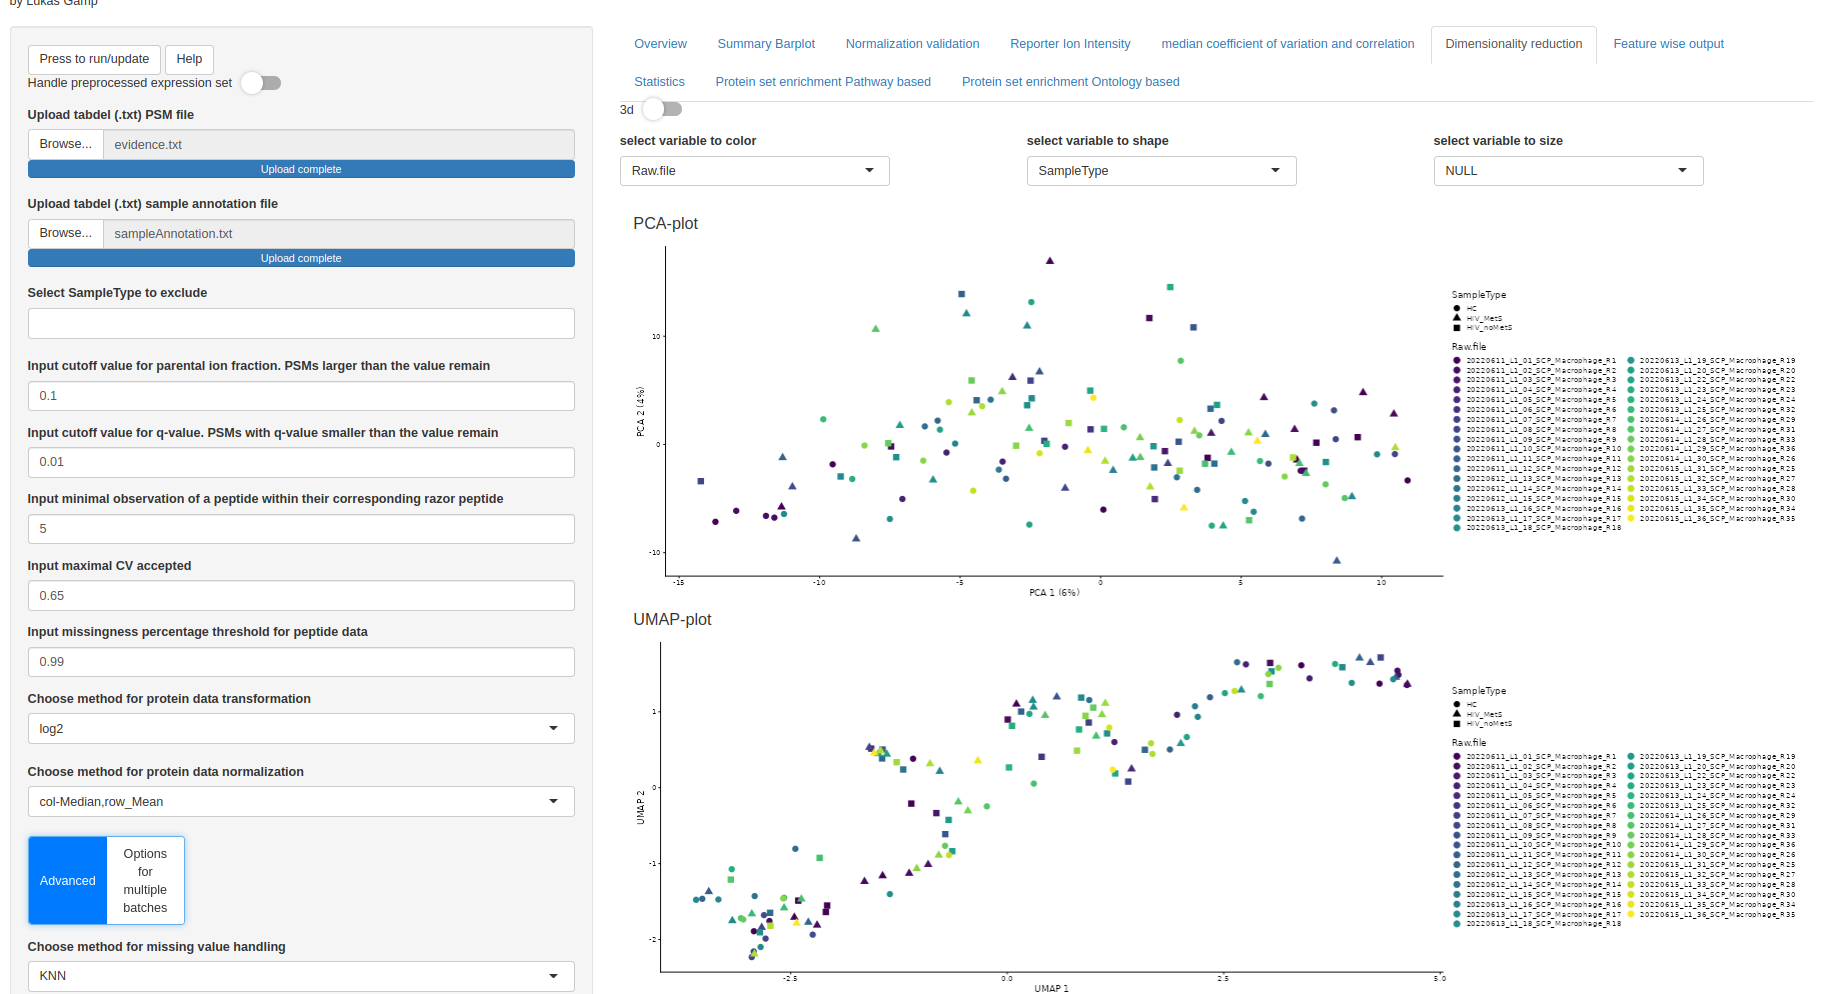
\includegraphics[width=1\linewidth]{screenshots/dim_red_batchC} 

}

\caption{Batch corrected dimensionality reduction analysis showcasing sample types (represented by shape) and raw files (represented by color). upper top: Principal Component Analysis (PCA). upper bottom: Uniform Manifold Approximation and Projection (UMAP). lower top: 3D Principal Component Analysis (PCA). lower bottom: 3D Uniform Manifold Approximation and Projection (UMAP)}\label{fig:ui_dim_red_batchC-1}
 \endfigure\egroup 
\bgroup  \origfigure[H] 

{\centering 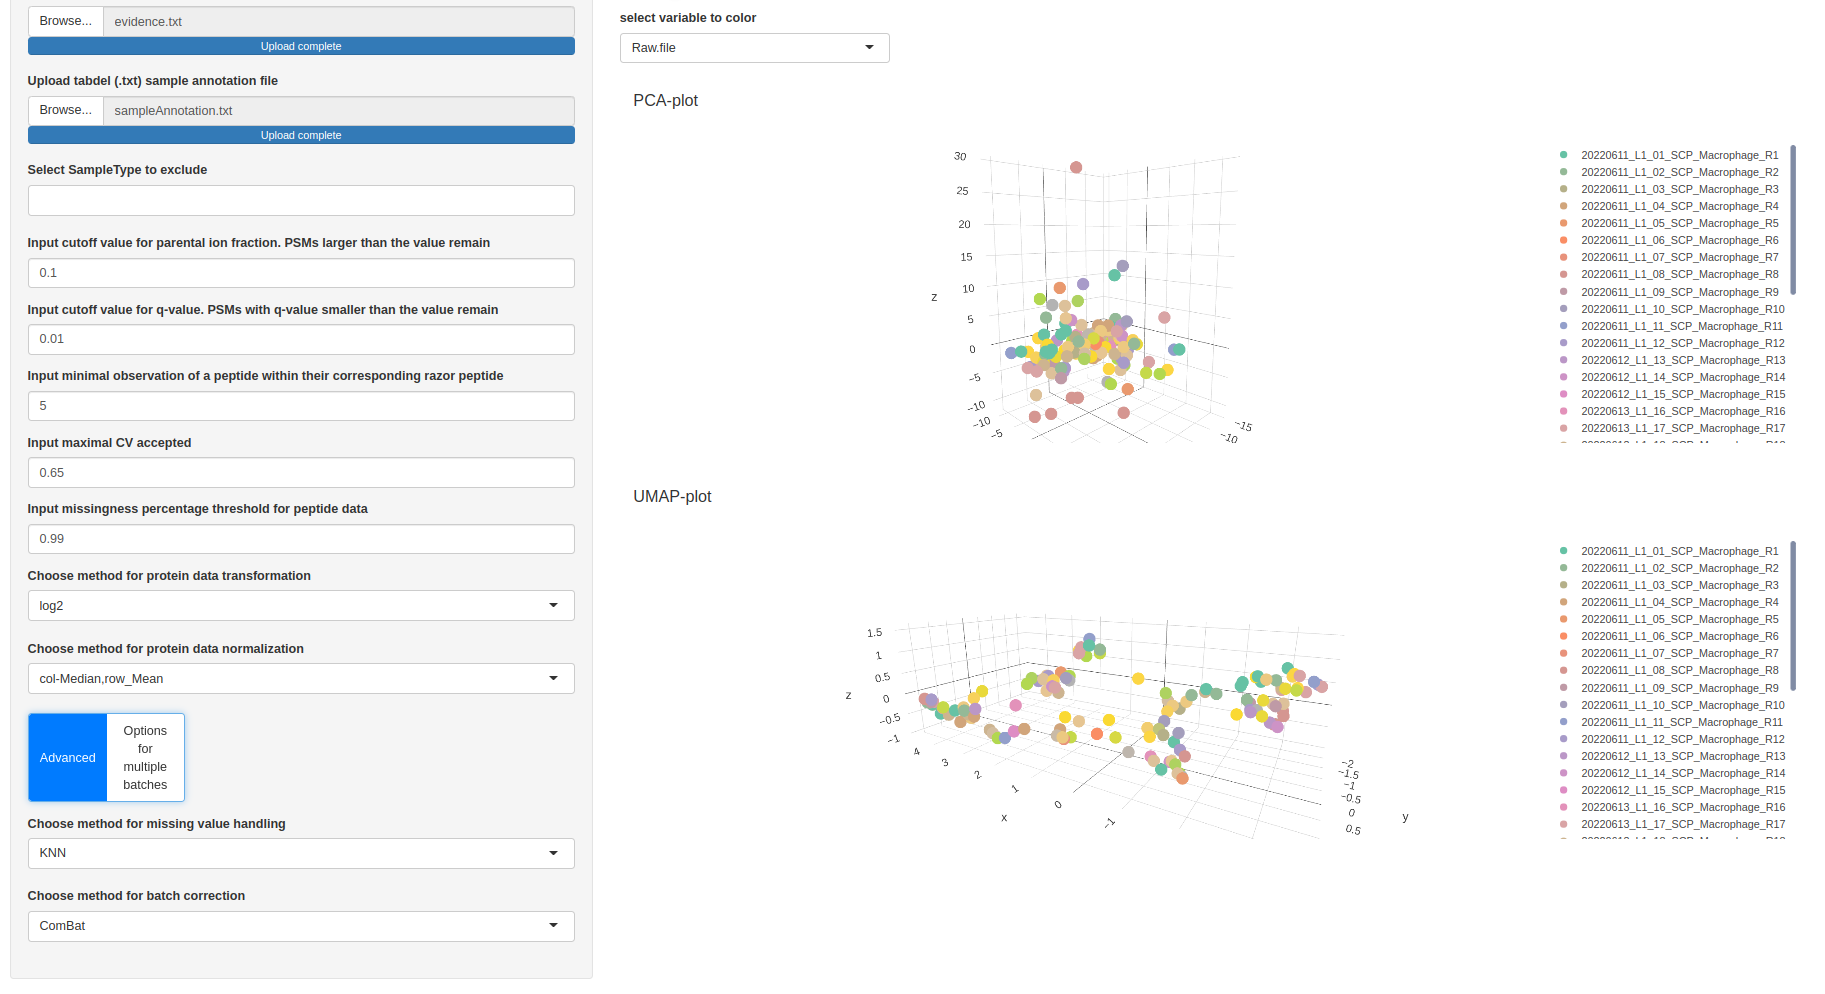
\includegraphics[width=1\linewidth]{screenshots/dim_red_batchC_3d} 

}

\caption{Batch corrected dimensionality reduction analysis showcasing sample types (represented by shape) and raw files (represented by color). upper top: Principal Component Analysis (PCA). upper bottom: Uniform Manifold Approximation and Projection (UMAP). lower top: 3D Principal Component Analysis (PCA). lower bottom: 3D Uniform Manifold Approximation and Projection (UMAP)}\label{fig:ui_dim_red_batchC-2}
 \endfigure\egroup

After applying batch correction using ComBat \citep{Leek2012}, neither
the 2D nor the 3D visualization demonstrates any noticeable effects
related to batches or sample types. The previously observed subtle
clustering of the first two batches is now eliminated, indicating
successful batch correction. However, it's important to note that the
default pipeline was executed without batch correction for correct
statistical testing.

\newpage
\bgroup  \origfigure[H] 

{\centering 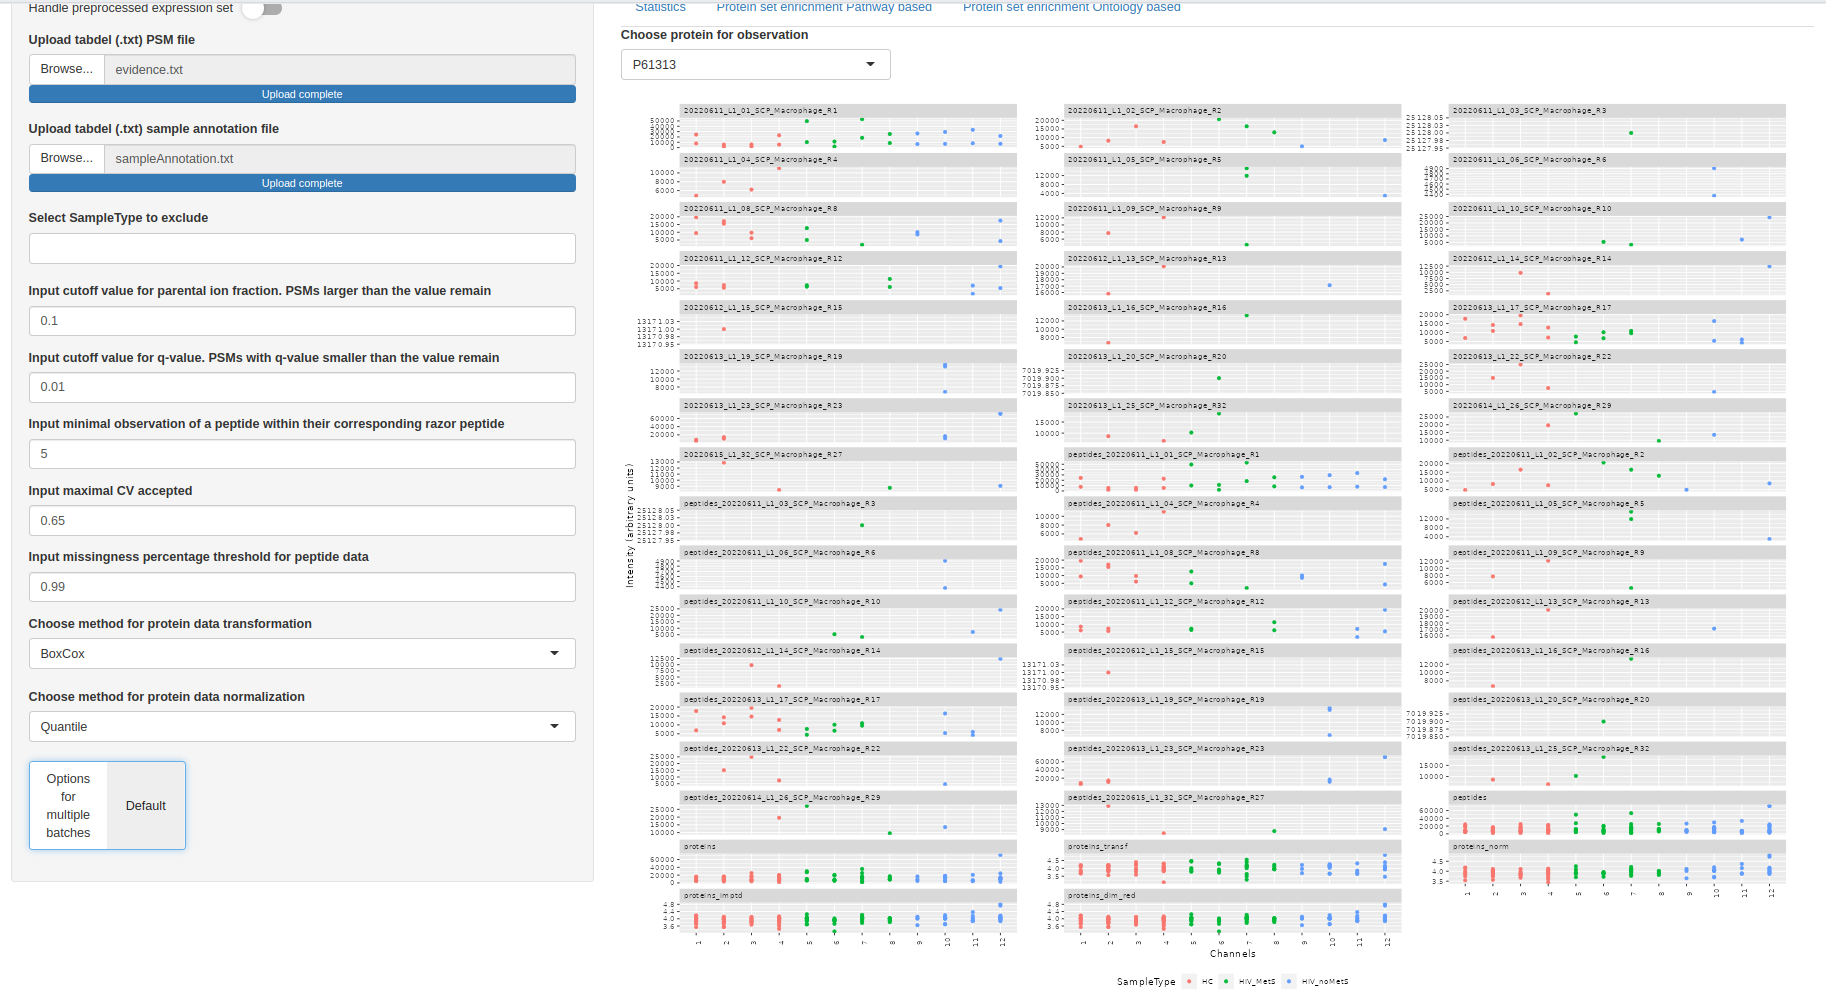
\includegraphics[width=1\linewidth]{screenshots/feature} 

}

\caption{Feature wise output for the protein P61313 (=60S ribosomal protein L15) over the course of the pipeline.}\label{fig:ui_feature}
 \endfigure\egroup

The scatter plots indicate the detected values associated with the
protein UniProt ID P61313 (= 60S ribosomal protein L15). Starting from
the peptide spectrum level and progressing to peptides aggregated for
individual raw files, these plots offer a comprehensive view of the
protein's peptide abundance across various batches. As indicated 14
batches show no abundance of peptides derived from the protein P61313 at
all. After merging the batches, the peptides appear to be abundant in
all channels.

\newpage
\bgroup  \origfigure[H] 

{\centering 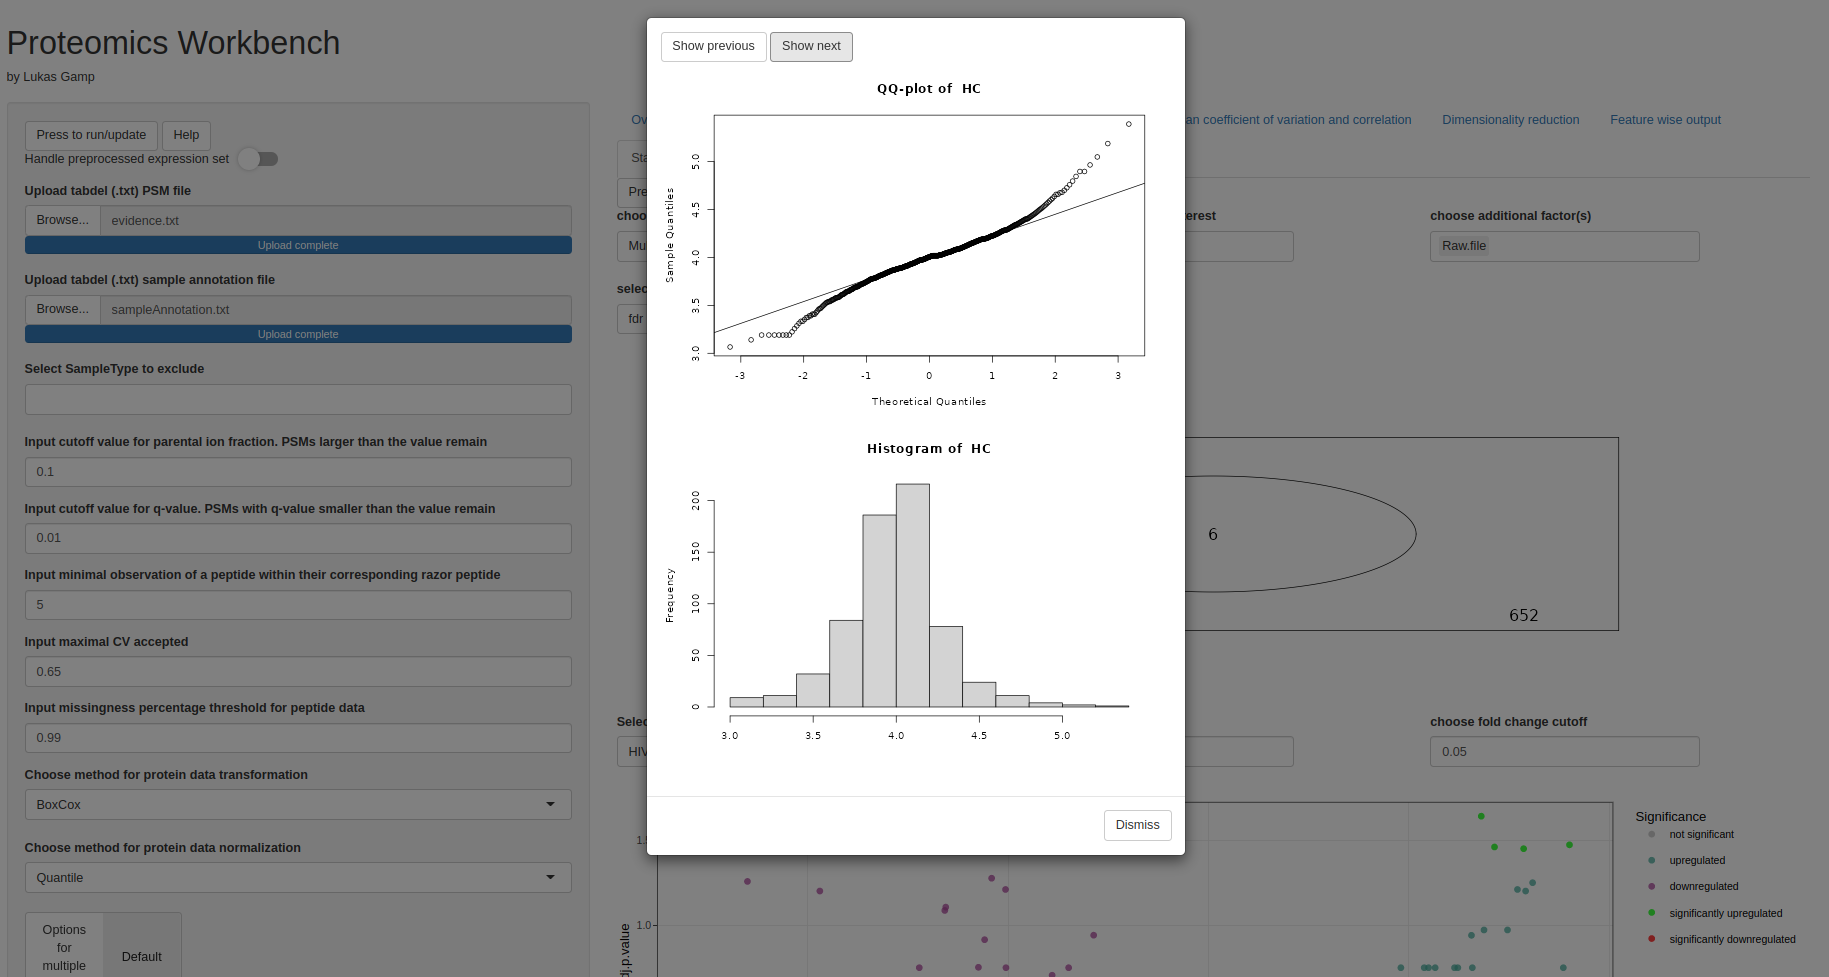
\includegraphics[width=1\linewidth]{screenshots/stat_dependency} 

}

\caption{Popup window for checking the dependency of the statistic module}\label{fig:ui_stat_dependency}
 \endfigure\egroup

The t-statistics employed in limma are known for their robustness in
handling non-normally distributed values. Nonetheless, it is recommended
for users to assess the distribution of their data based on sample types
before proceeding with statistical analysis. If the user is not
satisfied with the results or identifies any distributional issues, the
user can consider revisiting the transformation or normalization steps
to address any concerns or improve the data distribution prior to
statistical analysis.

The values for all sample types exhibit a unimodal distribution.
However, when examining the quantile-quantile (qq) plot, heavy tails can
be observed for all three groups. This indicates deviations from a
perfectly normal distribution, suggesting potential outliers in the
data.

\newpage
\bgroup  \origfigure[H] 

{\centering 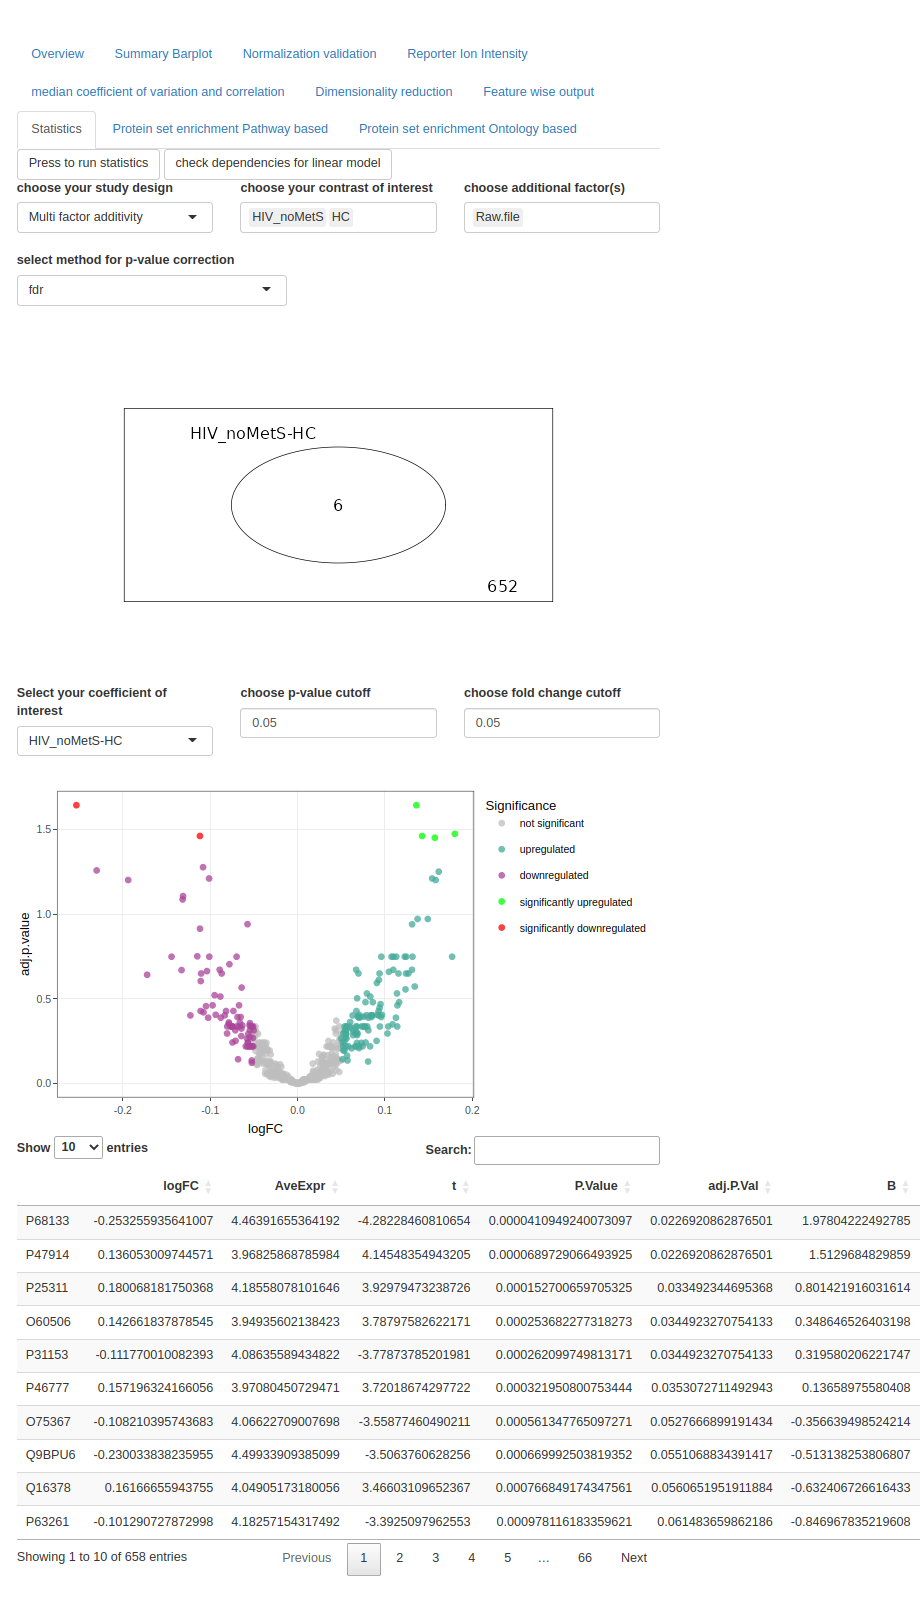
\includegraphics[width=0.7\linewidth]{screenshots/stat_HC_HIV_noMets} 

}

\caption{Statistic module}\label{fig:ui_stat_HC_HIV_noMets}
 \endfigure\egroup

\newpage

By comparing the log10-transformed and quantile-normalized expression
values between the HIV group without metabolic syndrome and the healthy
control (HC) group, six differentially expressed proteins were
identified. The Venndiagram indicates significantly up/downregulated
proteins. The Volcano represents -log10(adjusted p values) against log2
fold changes (logFC). These proteins include P68133 (Actin, alpha
skeletal muscle), P47914 (60S ribosomal protein L29), P25311
(Zinc-alpha-2-glycoprotein), O60506 (Heterogeneous nuclear
ribonucleoprotein Q), P31153 (S-adenosylmethionine synthase isoform
type-2), and P46777 (60S ribosomal protein L5). A total of 652 proteins
have been identified as not significantly upregulated or downregulated
in the comparison analysis. These proteins did not exhibit statistically
significant differences in expression between the compared groups or
conditions.

The direction of the contrast model determines the change in log-fold
change (logFC) values. For instance, in the depicted figure, P68133
(Actin, alpha skeletal muscle) shows an increased expression of 0.25
(25\%) in HIV\_noMetS macrophages compared to HC macrophages. It's
important to note that the logFC value changes by multiplication with -1
when the direction of the contrast model is reversed.

To account for potential batch effects, the batch factor was included as
a cofactor in the model, ensuring that any observed differential
expression is not confounded by batch variation.

\newpage
\bgroup  \origfigure[H] 

{\centering 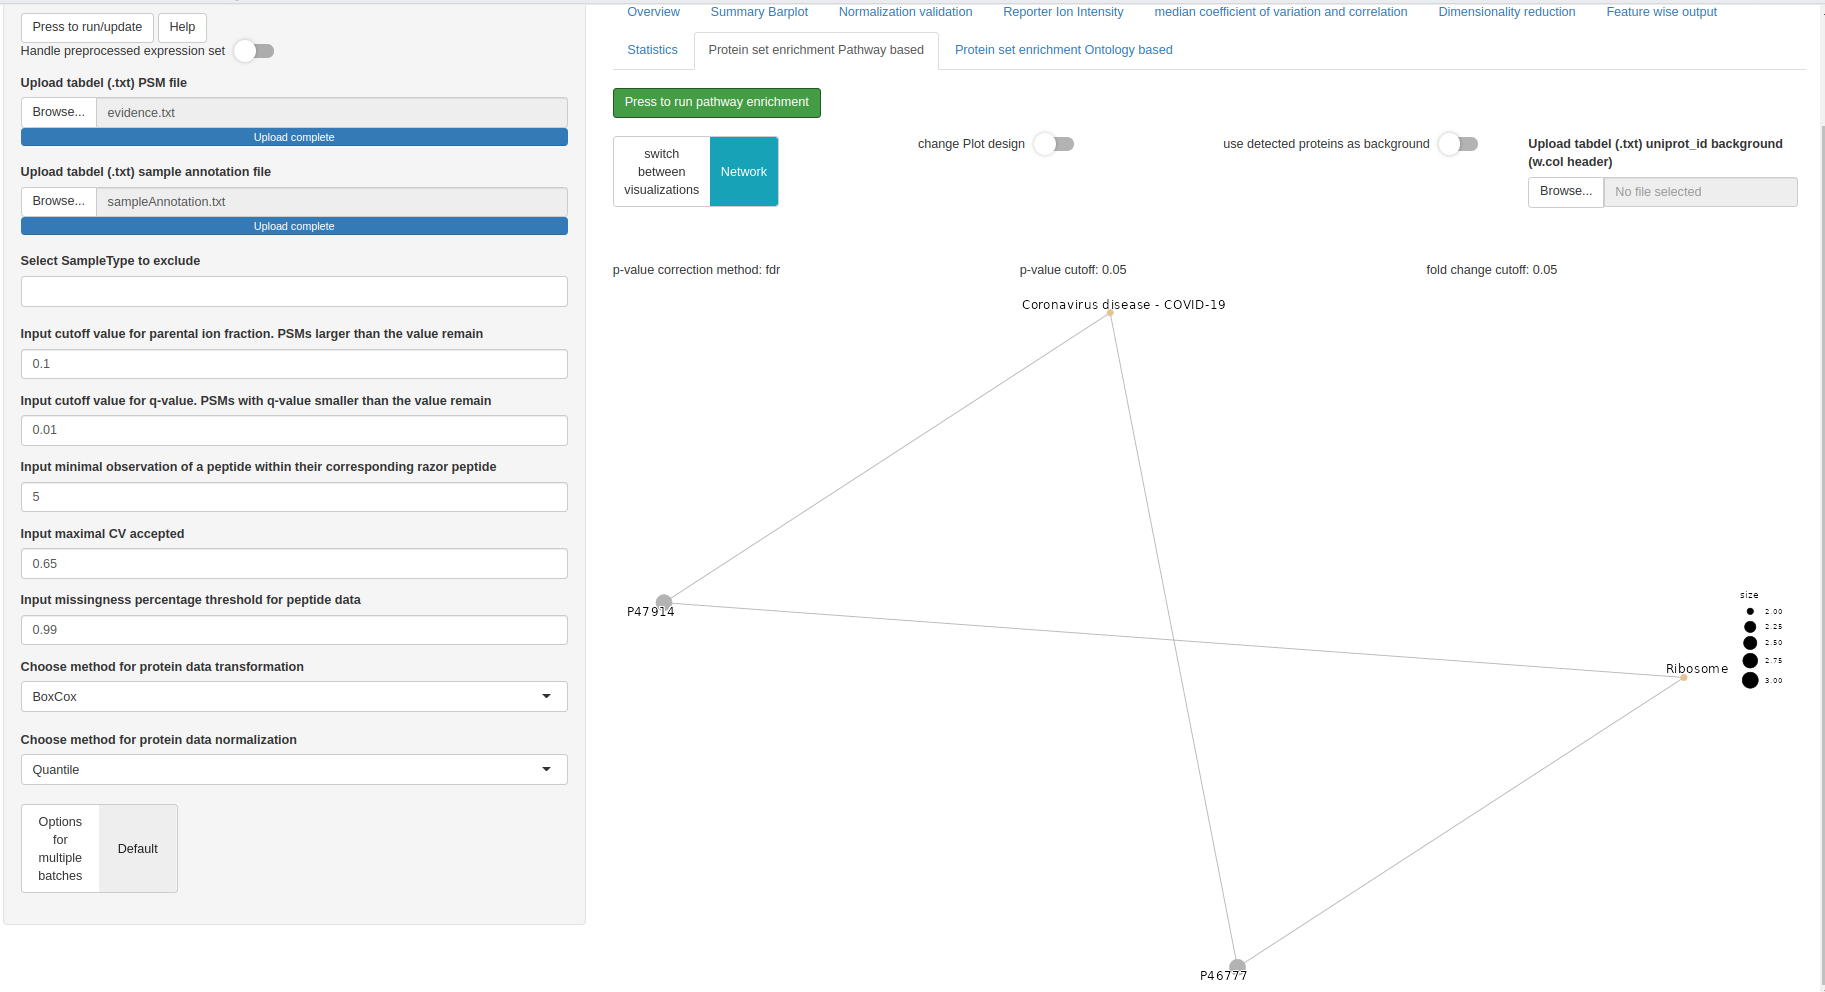
\includegraphics[width=0.9\linewidth]{screenshots/path_enrich_nw} 

}

\caption{Pathway enrichment. Networkplot indicating the association of differentially expressed proteins with pathways}\label{fig:ui_path_enrich_nw}
 \endfigure\egroup

The pathway enrichment mapped and tested with the exact Fisher test
\citep{Sprent2011} the differentially expressed proteins P46777 (60S
ribosomal protein L5) and P47914 (60S ribosomal protein L29) to the
ribosome and coronavirus disease (COVID-19) nodes.

\newpage
\bgroup  \origfigure[H] 

{\centering 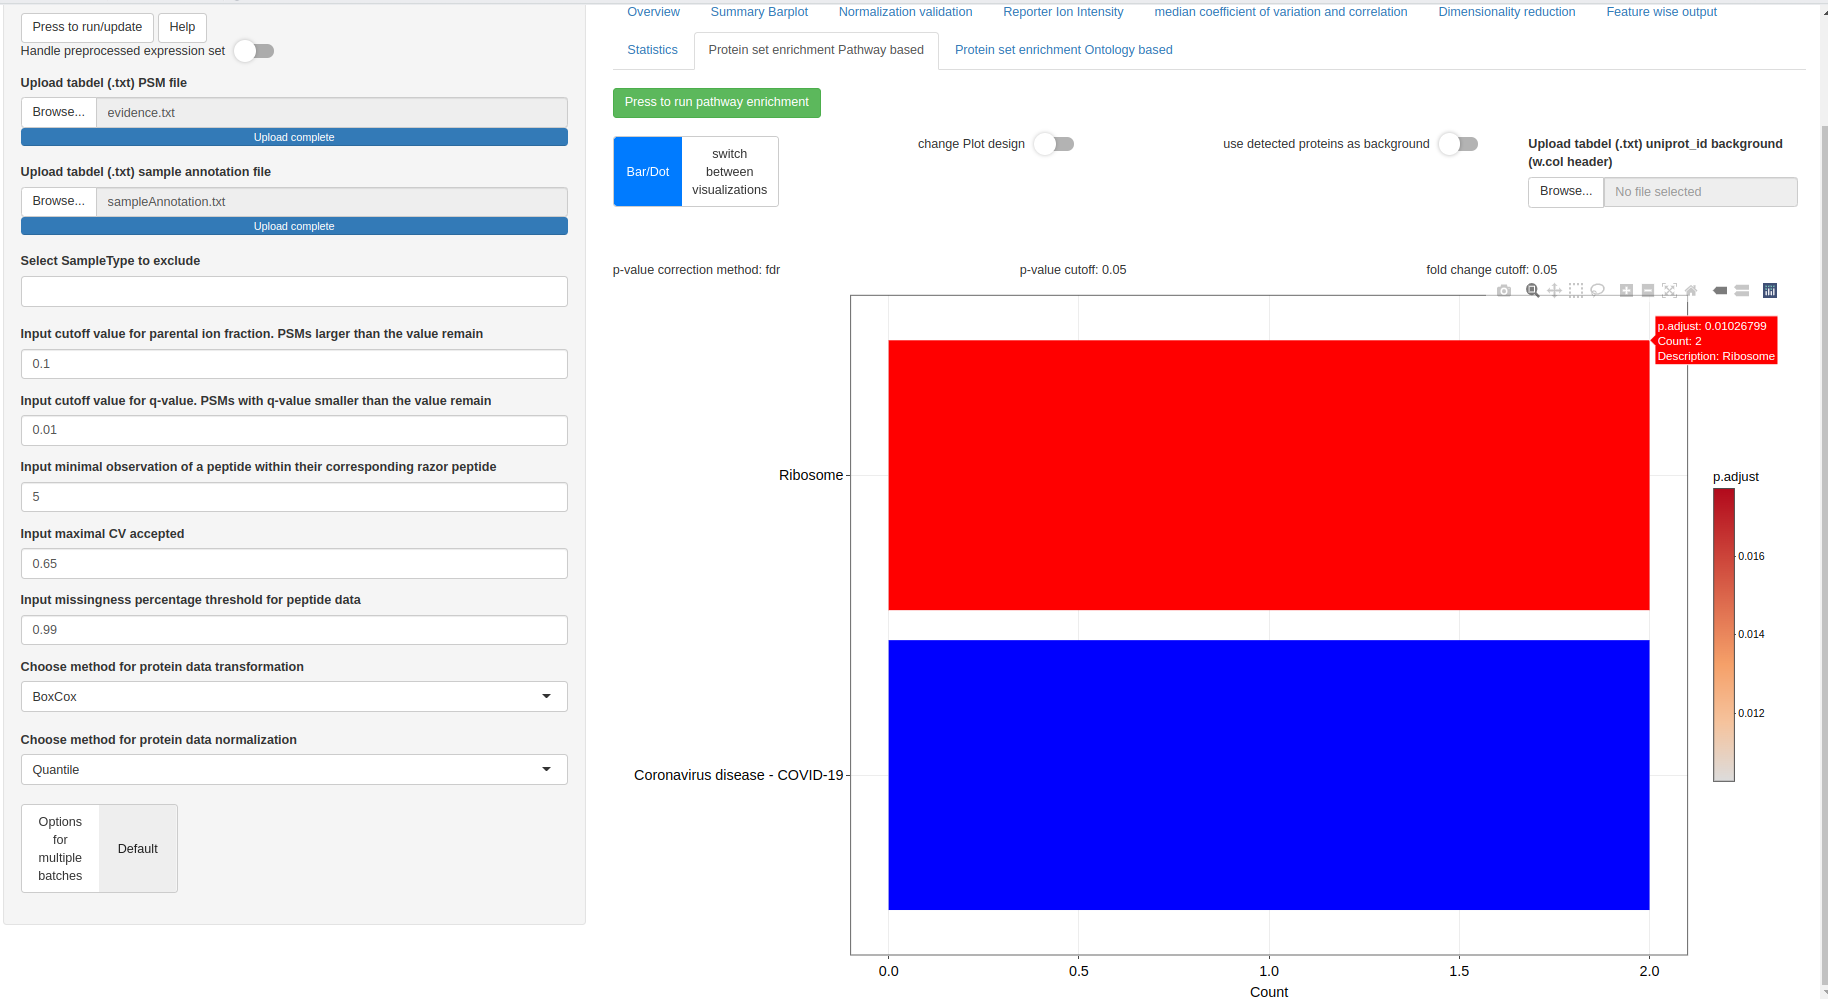
\includegraphics[width=0.9\linewidth]{screenshots/path_enrich_bar} 

}

\caption{Pathway enrichment. Barplot indicating the interaction significance of differentially expressed proteins}\label{fig:ui_path_enrich_bar}
 \endfigure\egroup

The barplot shows the significance of the two nodes. The count indicates
how many proteins are associated with the node of the network. When
hovering over the bar the user can read the p-value of the performed
Fisher test. The background for the statistical test can be chosen as
genome wide (default) or as the detected proteins. When choosing the
detected proteins as a background no pathway could be considered as
statistically significant.

\newpage
\bgroup  \origfigure[H] 

{\centering 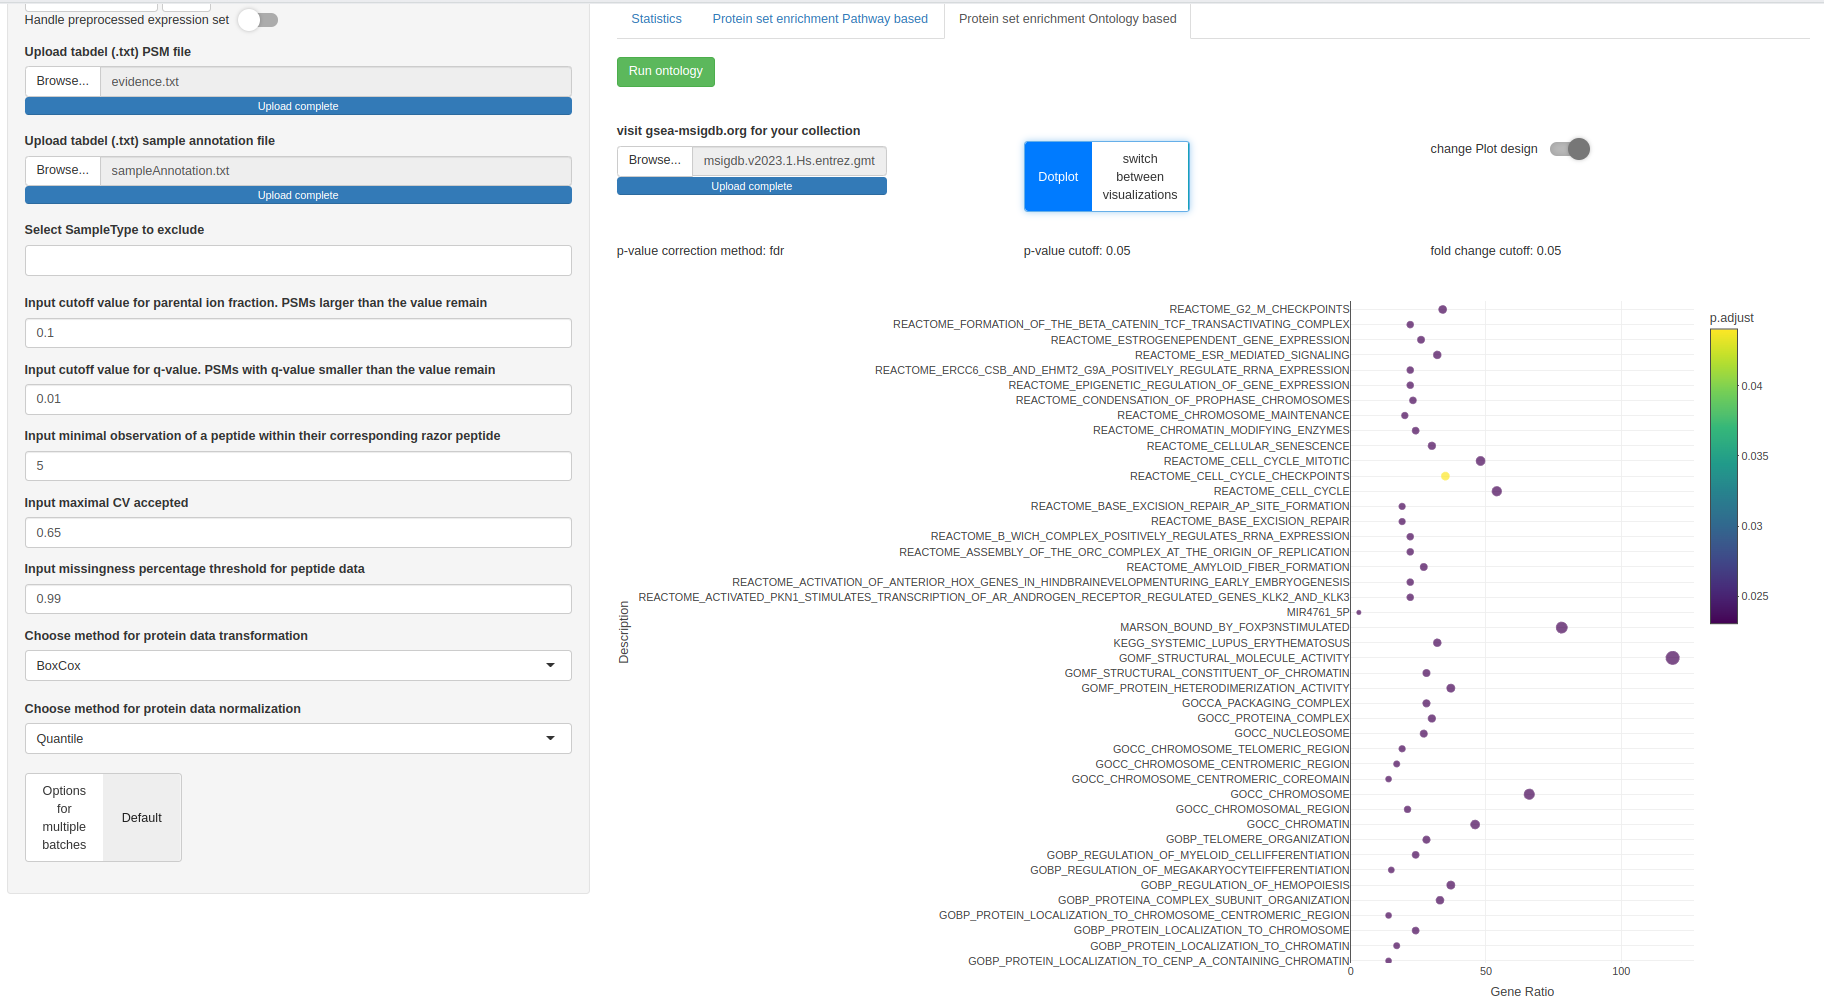
\includegraphics[width=0.9\linewidth]{screenshots/go_enrich_dot} 

}

\caption{Gene ontology enrichment against the complete human proteome. Snapshot dotplot indicating the interaction significance of found proteins}\label{fig:ui_go_enrich_bar}
 \endfigure\egroup

The position of the dot shows the number of matches for the particular
protein set. Colors indicate for the significance level. In this
analysis the entire repertoire of detected proteins was used and fetched
against the bundle containing all Human gene sets in the Human Molecular
Signatures Database (MSigDB). After a runtime of 3 minutes 672 of 24667
gene sets were found significantly over represented. Only the protein
set collections with the most protein matches were used (snipping tool
Plotly).

\newpage

\hypertarget{discussion}{%
\section{Discussion}\label{discussion}}

The Proteomics Workbench interface and the ProteoScanR pipeline
demonstrated how interactive engagement with the data not only enhances
the experience of biologists but also improves the comprehension of the
underlying significance of a biological dataset. By utilizing an
entropy-based visualization approach, the conservation of information
can be validated, allowing users to select appropriate methods and
adjust thresholds, cutoffs, and techniques accordingly. With the
selection of factors to indicate over multiple plots, biases can be
identified on various levels. Additionally, the analysis can be examined
on an individual protein basis, enabling the identification of
suspicious results. The statistics module provides users with a simple
tool to assess and visualize the results, offering clarity to dense
scatter plots through hover functions. Enrichment mapping links
statistically significant proteins to either the KEGG pathway database
or individual research data sets, depending on user selection. These
final results place the data in a biological context, which can be
explored interactively in graphical visualizations.

\hypertarget{interactive-pipeline}{%
\subsection{Interactive pipeline}\label{interactive-pipeline}}

Linear programming scripts are widely utilized for data analysis, and
R-shiny provides an efficient platform for implementing these scripts in
applications. This approach not only benefits scientists who are not
proficient in programming, but it is also convenient for programmers.
The Proteomics Workbench user interface offers a visually appealing
design, and the interactive menus enhance the user experience by
eliminating the need to search for specific lines of code on a black
screen. Modifying parameters of functions becomes effortless, and data
can be visualized without rerunning the entire script. R-shiny executes
functions on demand, which means that graphics, variables, and data
frames are not recalculated if their dependencies remain unchanged. This
feature makes the application both cost-effective and time-efficient.
The analysis pathway is visualized through multiple components,
providing users with a comprehensive view of the data. The overview
plot, generated using the Q-feature object-oriented programming in the
scp R library \citep{Vanderaa2021}, serves as a visual representation of
the analysis process. This plot allows users to track the progression of
the analysis and identify any missing files or samples.

\hypertarget{mutual-information}{%
\subsection{Mutual Information}\label{mutual-information}}

Information theory and the concept of mutual information provide a
framework for understanding the conservation of entropy in a dataset.
Traditionally, the validation of data transformation and normalization
methods has been limited to observing distributions through histograms
or Quantile-Quantile plots. However, the developed approach goes beyond
these conventional methods, providing a deeper context for the variation
in the data. By allowing users to choose the method that preserves the
maximum amount of information, the approach enables researchers to
extract the most valuable insights from their experiments. Normalization
methods play a crucial role in data analysis, and their selection
depends on the nature of the data and the specific analysis objectives.
The mutual information analysis revealed that quantile normalization
exhibited the smallest loss of entropy compared to other normalization
methods

\hypertarget{reporter-ion-intensity}{%
\subsection{Reporter ion intensity}\label{reporter-ion-intensity}}

MS2 reporter ion intensities can be effectively visualized using a
boxplot, where the medians represent the intensity distribution across
various factors such as sample type, batch, or channel. This
visualization aids users in assessing the variation and potential biases
in the dataset. During the example analysis, the reporter ion intensity
plot revealed inconsistencies in the dataset based on signal intensities
associated with different batches. It was observed that certain runs
exhibited a wide spread of signal intensities, which could indicate
technical issues or batch-related variations. These inconsistencies were
partly filtered out during the quality control process to ensure the
reliability and accuracy of the data.

\hypertarget{median-coefficient-of-variation}{%
\subsection{Median coefficient of
variation}\label{median-coefficient-of-variation}}

The median coefficient of variation (CV) was calculated for a razor
protein in relation to its ambiguous peptides. This statistical
parameter measures the variability of the razor protein's abundance
across different peptide measurements. The results were then visualized
using a boxplot, allowing users to assess the distribution of CV values
based on a selected factor. During testing and fine-tuning, the number
of observations for ambiguously matched peptides was adjusted to
evaluate its impact on the CV. By varying the number of observations,
researchers could determine the optimal parameter that yielded
meaningful CV values. In this context, the reference values from the
SCoPE2 publication \citep{Specht2021} were employed as benchmarks and
subjected to validation. The results showed that using a number of
observations of 5 for leading razor peptides was suitable for
identifying a cutoff value of 0.65. This cutoff value was determined by
observing the whiskers of the boxplots. By setting this threshold, noisy
peptides in the dataset could be effectively reduced, enhancing the
quality and reliability of the data.

\hypertarget{feature-wise-plot}{%
\subsection{Feature-wise plot}\label{feature-wise-plot}}

The feature-wise output plays a crucial role in enhancing the analysis
pathway by offering users the ability to select specific proteins and
explore their associated peptide spectra, peptide values, and protein
values throughout the analysis. This feature provides a detailed and
comprehensive view of the analysis results, enabling users to identify
any missing or erroneous data points, particularly in channels with low
or high abundance. By examining these individual protein profiles, users
can assess the quality of the wet lab work and detect any potential
errors or inconsistencies. In the case of observing the abundance of the
protein P61313 (60S ribosomal protein L15) over the entire course of the
experiment, it becomes apparent that there are missing values within
certain runs and channels. Specifically, 14 runs exhibit no signal for
this protein. This observation underscores the significance of
aggregating data at the peptide and protein levels and combining
individual runs to construct the final protein expression set. The
scattering of dots in the plot indicates the inflation of small values
and the deflation of large values after transformation. The scatter plot
of quantile normalized values demonstrates the processing steps taken
while preserving outliers and maintaining the biological relevance of
the data. This processing steps aid in achieving a more balanced
distribution of data and avoids the distortion of biological meaning.

\hypertarget{statistics-module}{%
\subsection{Statistics module}\label{statistics-module}}

The statistics module within the application provides users with a
user-friendly interface for hypothesis testing, even without prior
expertise in statistics. By leveraging the powerful R-package limma
\citep{Ritchie2015}, the module offers robust statistical analysis
methods, empowering users to perform tests and obtain results to
validate their hypotheses. One key feature of the statistics module is
its ability to handle multiple factors and therefore correct for batch
effects. Users can extend the statistical analysis across various
factors, allowing them to quantify the impact of different variables and
identify differentially expressed proteins. To enhance the user
experience, the visualization of statistical results has been improved,
resulting in visually appealing and interactive displays. These
visualizations enable users to explore and interpret the results
effortlessly, aiding in the comprehension of the statistical findings.
By providing intuitive and engaging visual representations, the module
facilitates the understanding and communication of complex statistical
analyses. When comparing the group HIV without metabolic syndrome and
the healthy control 6 proteins could be found as differentially
expressed after correcting the p-values by false discovery rate (FDR
\citep{Benjamini1995}). For example, the protein P68133 (Actin, alpha
skeletal muscle) exhibits a log fold change (logFC) of -0.25, indicating
a significant decrease in actin levels within the HIV group. This
finding aligns with previous publications suggesting that HIV exploits
cellular skeleton proteins and alters their expression levels
\citep{Turville2018}. By inducing orchestrated structural changes in
compartments composed of actin filaments, the virus facilitates its
spread and infects other lymphocytes \citep{Rodrigues2022}. Another
protein of interest, P47914 (60S ribosomal protein L29), demonstrates
the impact of viral infection on protein synthesis. Differential
expression of this protein further highlights the perturbations in
cellular processes caused by the virus.

\hypertarget{enrichment}{%
\subsection{Enrichment}\label{enrichment}}

The enrichment analysis module within the application addresses the
challenge of selecting protein sets for mapping by incorporating a
database-fetching functionality. This feature streamlines the enrichment
analysis process and eliminates the need for users to manually select
sets to map proteins against. The first variant of the enrichment
analysis module utilizes the KEGG database, which offers a comprehensive
collection of pathways and their interactions. By accessing this
database, users can gain valuable insights into the underlying pathways
and their relationships. This automated mapping against the KEGG
database provides a convenient and efficient way to perform enrichment
analysis. The second variant of the module caters to sophisticated users
who may have specific protein sets in mind based on their research
question. This flexibility allows users to select and incorporate their
own protein sets into the analysis, enabling research in multiple
contexts and providing a comprehensive insight into the dataset. Both
variants of the enrichment analysis module present the results in
interactive plots, offering users a dynamic and immersive experience
with the data. Users can explore the enriched pathways and interact with
the visualizations, gaining a deeper understanding of the relationships
and connections within the dataset. Additionally, if desired, users can
generate static plots and download them for use in presentations or
other offline contexts. As indicated by the statistical findings, the
KEGG enrichment analysis identified proteins associated with the
ribosome and COVID-19. Both protein sets were connected to two ribosomal
proteins, namely P47914 (60S ribosomal protein L29) and P46777 (60S
ribosomal protein L5). These findings align with the fact that HIV and
COVID-19, like all known viruses, depend entirely on the host cell's
translation machinery for protein synthesis. This includes utilizing the
host's ribosomes, tRNAs, amino acids, and all necessary factors for
protein synthesis initiation, elongation, and termination
\citep{Ohlmann2014}. Consequently, it is not surprising that these
ribosomal proteins were found to be abundant in HIV-infected
individuals.

\hypertarget{limitations}{%
\subsection{Limitations}\label{limitations}}

\bgroup  \origfigure[H] 

{\centering 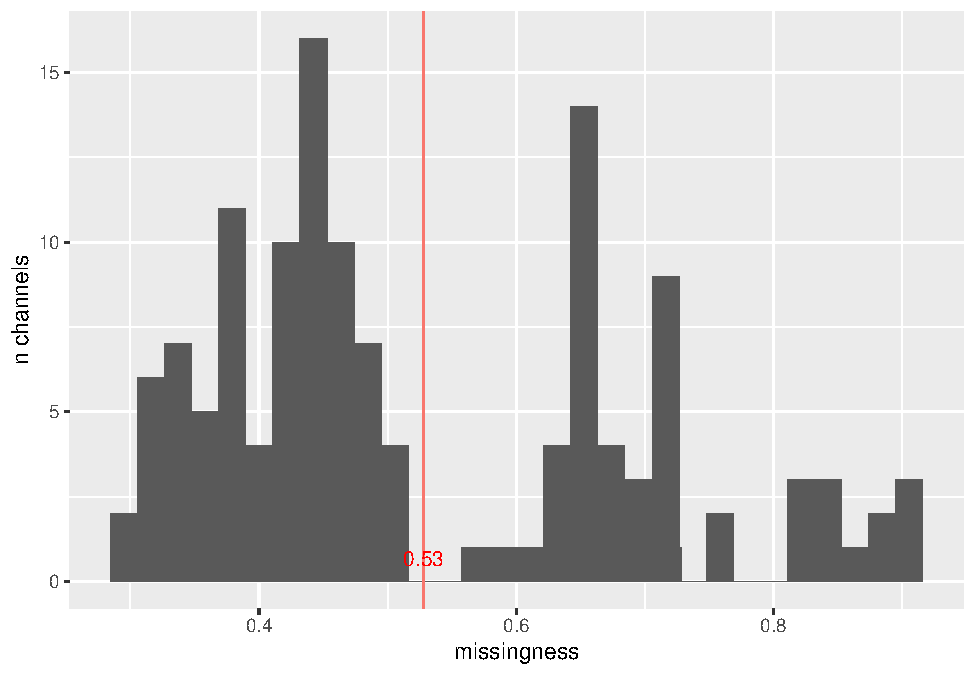
\includegraphics[width=0.9\linewidth]{Thesis_files/figure-latex/missingness-1} 

}

\caption{Missingness over channels. Y-axis: Height of the histogram bars show number of channels. X-axis: fraction of missing values. Red line: Mean of number of missing values over all runs}\label{fig:missingness}
 \endfigure\egroup

Unfortunately, a substantial number of individual proteins in the data
set (totaling 658) have missing values. On average, this amounts to
approximately 53\% of the proteins across all runs and channels. This
situation leads to the need for missing value imputation using
techniques such as k-nearest neighbor (K-NN), which can result in
averaged results. Additionally, it is important to note that this
imputation process can introduce potential loss of power in subsequent
statistical analysis. To improve future experiments, it is recommended
to increase the number of proteins in the carrier proteome. By expanding
the repertoire of proteins included in the carrier proteome, it can
enhance the coverage and depth of analysis, providing a more
comprehensive understanding of the biological system under
investigation. This can potentially lead to more robust and accurate
results in downstream analyses.

\hypertarget{future-perspectives}{%
\subsection{Future perspectives}\label{future-perspectives}}

\hypertarget{clustering-for-stratification-of-cells.}{%
\subsubsection{Clustering for stratification of
cells.}\label{clustering-for-stratification-of-cells.}}

The advantage of performing single-cell analysis lies in its ability to
provide a fine resolution of cellular differences. Unfortunately
variation causing effects such as cellular differentiation stages, are
mainly unknown when starting single-cell experiments. The next steps in
the development of the program aim to enable the stratification of
single-cell data sets. The analysis typically begins by finding clusters
within the datasets, identifying differentially expressed proteins, and
annotating cell types based on their expression profiles. Subsequently,
the analysis aims to distinguish sample types based on their expression
profiles.

Here I will explain how the analysis could start and elaborate the
limitations and challenges for this approach. Additional processing
steps will be included after the existing pipeline, so ProteoScanR
provides a starting point for further analysis.

\bgroup  \origfigure[H] 

{\centering \includegraphics[width=1\linewidth]{Thesis_files/figure-latex/cluster_analysis_dendrogram-1} 

}

\caption{Dendrogram showing the similarity over sample types. Tree was created using Ward`s minimum variance method.}\label{fig:cluster_analysis_dendrogram}
 \endfigure\egroup

As observed in the dendrogram, it is evident that sample type alone does
not account for the variation observed in the data. The branching
patterns in the dendrogram suggest that other factors might be
significant for contributing to the averaging of protein expression
levels. This can potentially lead to a decrease in the statistical power
of tests aimed at detecting differential expression between sample
types. Ideally, clustering approaches should result in individual
clusters that capture distinct sample types, enabling the testing of
differential expression within each cluster. This stratification of
samples within clusters allows for the identification of unique
expression patterns associated with specific biological variations. The
dendrogram, as demonstrated above, is an example of hierarchical
clustering, which provides a visual representation of the clustering
results. In this context, users should have the flexibility to select
the desired number of clusters that best explain the underlying
biological variation in their dataset. This allows for a more targeted
and precise analysis of differential expression within each cluster,
facilitating the identification of biologically meaningful patterns and
insights. To begin with the k-means clustering approach, it is crucial
to determine the optimal number of clusters before conducting the
analysis. This can be achieved using various approaches, one of which is
the gap statistic method \citep{Tibshirani2001}.

\bgroup  \origfigure[H] 

{\centering \includegraphics[width=0.9\linewidth]{Thesis_files/figure-latex/cluster_analysis_gap_stat-1} 

}

\caption{Optimal numbers of clusters calculated with gap statistics method}\label{fig:cluster_analysis_gap_stat}
 \endfigure\egroup

The gap statistic compares the total intracluster variation across
various values of k (number of clusters) to the expected variation under
a null reference distribution. The null reference distribution
represents a scenario where no clear clustering patterns exist in the
data. However as seen in the gap statistic a high number of clusters
will be difficult to distinguish from each other and explore the
biological meaning such as differentiation in the example macrophage
dataset. Another approach used to determine the optimal number of
clusters is the silhouette method.

\bgroup  \origfigure[H] 

{\centering \includegraphics[width=0.9\linewidth]{Thesis_files/figure-latex/cluster_analysis_silh-1} 

}

\caption{Optimal number of clusters calculated with silhoutte method.}\label{fig:cluster_analysis_silh}
 \endfigure\egroup

The silhouette method calculates silhouette coefficients for each data
point, which quantify how closely the point resembles its own cluster
compared to other clusters. If the overall distances between clusters
are small, indicating overlapping or unclear separation, it is suggested
to take the minimum k. This suggests that the data points may not be
well-separated into distinct clusters. As suggested by the silhouette
method in this case a lower number of clusters to differentiate cell
types is recommended.

\bgroup  \origfigure[H] 

{\centering \includegraphics[width=0.9\linewidth]{Thesis_files/figure-latex/cluster_analysis_dim_red-1} 

}

\caption{PCA plot with cluster indication. Shape of the datapoints indicate sample types. Clusters are encircled and color coded.}\label{fig:cluster_analysis_dim_red}
 \endfigure\egroup

As seen in the principal components analysis, clusters are densely
packed, and the plot shows no clear differentiation between the 8
suggested clusters. The dense packing and poor resolution indicates that
other factors may be influencing the lack of distinct separation. One of
the other factors involves the large number of imputed values due the
high rate of missing values in the protein expression set. K-NN is not
able to impute biological differences and therefore averages the
particular missing value by its k neighbors.

This suggests the utilization of a different data set for developing the
clustering module of the future program. By employing a data set with a
lower rate of missing values in the protein expression set, the accuracy
and reliability of the clustering analysis can be enhanced. Having a
data set with less missing data will allow for a more precise
identification of clusters and differentiation between cell types.

\hypertarget{machine-learning}{%
\subsubsection{Machine learning}\label{machine-learning}}

One potential target for future research could involve leveraging
artificial intelligence techniques to predict cellular behavior, cell
types, or even diseases. By running the application on a server and
creating a database, it would be possible to harness the power of AI
algorithms such as decision trees, random forests, or support vector
machines. Applying artificial intelligence to biological data has the
potential to enhance the classification of cell types, similar to the
earlier discussed clustering approach. However, it is important to note
that training and validating these algorithms typically requires
supervision and can be a time-consuming task.

Another area of focus, not limited to research topics, could be to
enhance the usability of the application. While a development time of 5
months for the pipeline and user interface is sufficient to meet the
analytical needs, there is always room for improvement in terms of
user-friendliness. It is essential to consider the needs of all users,
including the least experienced user. To prevent program crashes and
errors, it may be necessary to implement try-catch around code blocks,
as well as validate-need statements for the validation of user input.
Additionally, creating a user-friendly environment involves establishing
effective channels of communication between users and developers, such
as utilizing platforms like GitHub for collaboration and feedback.

\newpage

\hypertarget{conclusion}{%
\section{Conclusion}\label{conclusion}}

Through this project, I demonstrated that computational analysis can be
made accessible to a wide range of biologists by providing an
interactive environment. It is important to recognize that there cannot
be a one-size-fits-all approach for proteomics datasets. Therefore, the
application offers easy-to-interpret visualizations that allow users to
assess the patterns and trends in their observed datasets. The default
options provided in the application are based on successful analysis
pipelines such as ScoPE2 \citep{Specht2021}, serving as a starting point
for customization at multiple levels.

The example dataset provided showcases the inherent challenges in
proteomic data analysis. It exhibits skewed distributions, batch
effects, and a substantial number of missing values. Despite these
complexities, the ProteoScanR pipeline and Proteomics Workbench
interface offer biologists a convenient means to address their research
questions and validate the computations performed. The example use case
also sheds light on the fact that previous proteomics publications, such
as the ScoPE2 study \citep{Specht2021}, may not always employ the gold
standard in data processing. This emphasizes the importance of
critically evaluating and refining data processing steps through trial
and error to achieve optimal results. The interactive environment
provided by the application allows users to navigate the trial and error
process without experiencing frustration. This user-friendly interface
ensures that researchers can iteratively refine their data processing
steps and analyze the results in a seamless manner. Furthermore, the
scalability of the application was initially unknown until the final
submission of the single-cell dataset. The programming and testing of
the application primarily focused on bulk datasets, typically consisting
of up to four runs at once. However, it is noteworthy that the
application demonstrates remarkable efficiency and performance, even
when running large datasets. The ability of the application to
efficiently handle larger datasets, such as single-cell studies, is a
significant advantage. It allows researchers to analyze complex and
extensive datasets without sacrificing performance or compromising the
quality of the results. This scalability makes the application a
valuable tool for analyzing diverse types of biological data,
accommodating the needs of researchers working with both smaller and
larger datasets.

ProteoScanR pipeline and Proteomics Workbench user interface serve as
valuable tools for individual researchers and research communities,
enabling them to analyze and visualize their data in meetings, even on
non-performant computers. However, one of the future perspectives
involves deploying the application on a server, making it accessible to
research groups around the world. This would enhance collaboration and
facilitate the sharing of insights and findings across different
geographical locations. By providing a centralized platform for
proteomics analysis, aiming to foster scientific advancements and enable
researchers to make significant contributions to their respective
fields. Furthermore by having a central hub for proteomic data analysis
and the use of artificial intelligence the biological meaning could be
brought to a wider context. Since proteomic data could be saved without
violating data protection laws, algorithms could be employed to learn
from large datasets.

An important aspect of learning from the data involves annotating
specimens, particularly in the context of single-cell proteomics. The
clustering approach is a primary focus for future development and
analysis in the near term. By employing clustering algorithms and
stratifying the data, individual cells can be labeled and annotated
based on their phenotypes. This annotation process involves associating
protein sets collections with specific clusters or cell types, providing
a more comprehensive understanding of cellular heterogeneity and
functional characteristics.

In conclusion, the ProteoScanR pipeline and Proteomics Workbench
interface provide a user-friendly and efficient approach for proteomic
data analysis, enabling biologists to address their research questions
and validate computations. Future perspectives include deploying the
application on a server for global accessibility, leveraging artificial
intelligence techniques, and implementing clustering approaches to
further enhance annotation and understanding of cellular heterogeneity
and functional characteristics.

\newpage

\bibliography{bibliography}

\newpage

\hypertarget{appendix}{%
\section{Appendix}\label{appendix}}

\hypertarget{wet-lab}{%
\subsection{Wet lab}\label{wet-lab}}

\hypertarget{cells-sorting-protocol}{%
\subsubsection{Cells sorting protocol}\label{cells-sorting-protocol}}

\begin{enumerate}
\item 96 single cells from each donor were sorted into a single plate. Each well contained a single cell. As such, 12 different plates containing single cells from 12 different donors were prepared. 
\item Carrier plates were also prepared. In the carrier plates, 100 cells from one donor were sorted into each well. 24 such wells (3 columns) were prepared for each donor.
\end{enumerate}

\hypertarget{digestion-protocol}{%
\subsubsection{Digestion protocol}\label{digestion-protocol}}

\begin{enumerate}
\item Prepare 25 ng/ $\mu$L trypsin in 100 mmol/L Triethylammonium bicarbonate buffer (TEAB).
\item Add 25 ng/$\mu$L trypsin: 2 $\mu$L to the carrier samples, 1 $\mu$L to the single cell samples.
\item Seal the plates.
\item Centrifuge (2 min at 120 G).
\item Incubate overnight at 37 °C.
\end{enumerate}

\hypertarget{labeling-protocol}{%
\subsubsection{Labeling protocol}\label{labeling-protocol}}

\begin{enumerate}
\item Let the TMTpro labels come to room temperature so that all the condensation on the tube is gone. Dissolve the TMTpro reagents in anhydrous acetonitril (ACN) to obtain a concentration of 10 $\mu$g/$\mu$L.
\item Add 1 $\mu$L of TMTpro reagents according to the tables. For one set of plates, you will need 16 $\mu$L of each label. It is recommended to aliquot a slightly larger volume, around 20 $\mu$L.
\item Seal the plates.
\item Centrifuge for 2 minutes at 120 G.
\item Incubate for 1 hour at room temperature.
\item Prepare a 5% hydroxylamine solution in water.
\item Add 1 $\mu$L of the 5% hydroxylamine solution to each well.
\item Seal the plates.
\item Centrifuge for 2 minutes at 120 G.
\item Incubate for 1 hour at room temperature.
\item Cover the plates with cap strips.
\end{enumerate}

\hypertarget{pooling-protocol}{%
\subsubsection{Pooling protocol}\label{pooling-protocol}}

\begin{enumerate}
\item Wash a 10 $\mu$L glass microsyringe five times with ACN.
\item Use the microsyringe to combine TMTpro-labeled samples into 36 LC autosampler vials with built-in glass inserts.
\item Combine six carrier wells from each sample and add the carrier proteome to the 36 TMTpro sets.
\item Combine the first set by taking well A1 from the first single-cell plate, well A2 from the second plate, well A3 from the third plate, and so on. For the next set, take well A1 from the second plate, well A2 from the third plate, and so on. Combine 12 sets following this scheme. Combine the next 24 sets by following the same scheme for rows B and C.
\item Vacuum centrifuge the combined sets to dryness.
\item Dissolve the dried samples in 7 $\mu$L of buffer A and transfer them to LC-MS/MS for further analysis.
\end{enumerate}

\hypertarget{dry-lab}{%
\subsection{Dry lab}\label{dry-lab}}

\hypertarget{r-version-info}{%
\subsubsection{R-version info}\label{r-version-info}}

\begin{verbatim}
R version 4.3.0 (2023-04-21)
Platform: x86_64-pc-linux-gnu (64-bit)
Running under: Ubuntu 22.04.2 LTS

 [1] visNetwork_2.1.2            snowfall_1.84-6.2          
 [3] snow_0.4-4                  piano_2.16.0               
 [5] org.Hs.eg.db_3.17.0         AnnotationDbi_1.62.1       
 [7] infotheo_1.2.0.1            clusterProfiler_4.8.1      
 [9] plotly_4.10.1               sva_3.48.0                 
[11] BiocParallel_1.34.2         genefilter_1.82.1          
[13] mgcv_1.8-42                 nlme_3.1-162               
[15] impute_1.74.1               CONSTANd_1.8.0             
[17] limma_3.56.1                scater_1.28.0              
[19] scuttle_1.10.1              reshape2_1.4.4             
[21] dplyr_1.1.2                 magrittr_2.0.3             
[23] ggplot2_3.4.2               SingleCellExperiment_1.22.0
[25] scp_1.10.0                  QFeatures_1.10.0           
[27] MultiAssayExperiment_1.26.0 SummarizedExperiment_1.30.1
[29] Biobase_2.60.0              GenomicRanges_1.52.0       
[31] GenomeInfoDb_1.36.0         IRanges_2.34.0             
[33] S4Vectors_0.38.1            BiocGenerics_0.46.0        
[35] MatrixGenerics_1.12.0       matrixStats_0.63.0         
[37] spsComps_0.3.2.1            DT_0.28                    
[39] shinydashboard_0.7.2        shinyWidgets_0.7.6         
[41] shiny_1.7.4                
\end{verbatim}

\newpage
\listoffigures

\end{document}
